\documentclass[11pt,a4paper,oneside]{report}

% thanks to http://tex.stackexchange.com/a/47579/71109
\usepackage{ifxetex}
\usepackage{ifluatex}
\newif\ifxetexorluatex % a new conditional starts as false
\ifnum 0\ifxetex 1\fi\ifluatex 1\fi>0
   \xetexorluatextrue
\fi

\ifxetexorluatex
  \usepackage{fontspec}
\else
  \usepackage[T1]{fontenc}
  \usepackage[utf8]{inputenc}
  \usepackage[lighttt]{lmodern}
\fi

\usepackage[english,magyar]{babel} % Alapértelmezés szerint utoljára definiált nyelv lesz aktív, de később külön beállítjuk az aktív nyelvet.

%\usepackage{cmap}
\usepackage{amsfonts,amsmath,amssymb} % Mathematical symbols.
%\usepackage[ruled,boxed,resetcount,linesnumbered]{algorithm2e} % For pseudocodes. % beware: this is not compatible with LuaLaTeX, see http://tex.stackexchange.com/questions/34814/lualatex-and-algorithm2e
\usepackage{booktabs} % For publication quality tables for LaTeX
\usepackage{graphicx}

%\usepackage{fancyhdr}
%\usepackage{lastpage}

\usepackage{anysize}
%\usepackage{sectsty}
\usepackage{setspace} % For setting line spacing

\usepackage[unicode]{hyperref} % For hyperlinks in the generated document.
\usepackage{xcolor}
\usepackage{listings} % For source code snippets.

\usepackage[amsmath,thmmarks]{ntheorem} % Theorem-like environments.

\usepackage[hang]{caption}

\singlespacing

\newcommand{\selecthungarian}{
	\selectlanguage{magyar}
	\setlength{\parindent}{2em}
	\setlength{\parskip}{0em}
	\frenchspacing
}

\newcommand{\selectenglish}{
	\selectlanguage{english}
	\setlength{\parindent}{0em}
	\setlength{\parskip}{0.5em}
	\nonfrenchspacing
	\renewcommand{\figureautorefname}{Figure}
	\renewcommand{\tableautorefname}{Table}
	\renewcommand{\partautorefname}{Part}
	\renewcommand{\chapterautorefname}{Chapter}
	\renewcommand{\sectionautorefname}{Section}
	\renewcommand{\subsectionautorefname}{Section}
	\renewcommand{\subsubsectionautorefname}{Section}
}

\usepackage[numbers]{natbib}
\usepackage{xspace}

\newcommand{\vikszerzoVezeteknev}{Ghadri}
\newcommand{\vikszerzoKeresztnev}{Najib}

\newcommand{\vikkonzulensAMegszolitas}{}
\newcommand{\vikkonzulensAVezeteknev}{Szemenyei}
\newcommand{\vikkonzulensAKeresztnev}{Márton}

\newcommand{\vikkonzulensBMegszolitas}{}
\newcommand{\vikkonzulensBVezeteknev}{}
\newcommand{\vikkonzulensBKeresztnev}{}

\newcommand{\vikcim}{Driving Scene Understanding in Simulation with 
Stereo RGB imaging and CNN synergy} 
\newcommand{\viktanszek}{\bmeiit} 
\newcommand{\vikdoktipus}{\msc} 
\newcommand{\vikmunkatipusat}{szakdolgozatot} % a "hallgató nyilatkozat"

\newcommand{\szerzoMeta}{\vikszerzoVezeteknev{} \vikszerzoKeresztnev}

\newcommand{\bme}{Budapest University of Technology and Economics}
\newcommand{\vik}{Faculty of Electrical Engineering and Informatics}

\newcommand{\bmeiit}{Department of Control Engineering and Information Technology}

\newcommand{\keszitette}{Author}
\newcommand{\konzulens}{Advisor}

\newcommand{\bsc}{Bachelor's Thesis}
\newcommand{\msc}{Master's Thesis}
\newcommand{\tdk}{Scientific Students' Association Report}
\newcommand{\bsconlab}{BSc Project Laboratory}
\newcommand{\msconlabi}{MSc Project Laboratory 1}
\newcommand{\msconlabii}{MSc Project Laboratory 2}

\newcommand{\pelda}{Example}
\newcommand{\definicio}{Definition}
\newcommand{\tetel}{Theorem}

\newcommand{\bevezetes}{Introduction}
\newcommand{\koszonetnyilvanitas}{Acknowledgements}
\newcommand{\fuggelek}{Appendix}

% Optional custom titles
%\addto\captionsenglish{%
%\renewcommand*{\listfigurename}{Your list of figures title}
%\renewcommand*{\listtablename}{Your list of tables title}
%\renewcommand*{\bibname}{Your bibliography title}
%}

\newcommand{\szerzo}{\vikszerzoKeresztnev{} \vikszerzoVezeteknev}
\newcommand{\vikkonzulensA}{\vikkonzulensAMegszolitas\vikkonzulensAKeresztnev{} \vikkonzulensAVezeteknev}
\newcommand{\vikkonzulensB}{\vikkonzulensBMegszolitas\vikkonzulensBKeresztnev{} \vikkonzulensBVezeteknev}
\newcommand{\vikkonzulensC}{\vikkonzulensCMegszolitas\vikkonzulensCKeresztnev{} \vikkonzulensCVezeteknev}

\newcommand{\selectthesislanguage}{\selectenglish}

\bibliographystyle{plainnat}

\newcommand{\ie}{i.e.\@\xspace}
\newcommand{\Ie}{I.e.\@\xspace}
\newcommand{\eg}{e.g.\@\xspace}
\newcommand{\Eg}{E.g.\@\xspace}
\newcommand{\etal}{et al.\@\xspace}
\newcommand{\etc}{etc.\@\xspace}
\newcommand{\vs}{vs.\@\xspace}
\newcommand{\viz}{viz.\@\xspace} % videlicet
\newcommand{\cf}{cf.\@\xspace} % confer
\newcommand{\Cf}{Cf.\@\xspace}
\newcommand{\wrt}{w.r.t.\@\xspace} % with respect to
\newcommand{\approximately}{approx.\@\xspace}

\newcommand{\appendixnumber}{1}  % a fofejezet-szamlalo az angol ABC 1. betuje (A) lesz

%--------------------------------------------------------------------------------------
% Page layout setup
%--------------------------------------------------------------------------------------
% we need to redefine the pagestyle plain
% another possibility is to use the body of this command without \fancypagestyle
% and use \pagestyle{fancy} but in that case the special pages
% (like the ToC, the References, and the Chapter pages)remain in plane style

\pagestyle{plain}
\marginsize{35mm}{25mm}{15mm}{15mm}

\setcounter{tocdepth}{3}
%\sectionfont{\large\upshape\bfseries}
\setcounter{secnumdepth}{3}

\sloppy % Margón túllógó sorok tiltása.
\widowpenalty=10000 \clubpenalty=10000 %A fattyú- és árvasorok elkerülése
\def\hyph{-\penalty0\hskip0pt\relax} % Kötőjeles szavak elválasztásának engedélyezése


%--------------------------------------------------------------------------------------
% Setup hyperref package
%--------------------------------------------------------------------------------------
\hypersetup{
    % bookmarks=true,            % show bookmarks bar?
    unicode=true,              % non-Latin characters in Acrobat's bookmarks
    pdftitle={\vikcim},        % title
    pdfauthor={\szerzoMeta},    % author
    pdfsubject={\vikdoktipus}, % subject of the document
    pdfcreator={\szerzoMeta},   % creator of the document
    pdfproducer={},    % producer of the document
    pdfkeywords={},    % list of keywords (separate then by comma)
    pdfnewwindow=true,         % links in new window
    colorlinks=true,           % false: boxed links; true: colored links
    linkcolor=black,           % color of internal links
    citecolor=black,           % color of links to bibliography
    filecolor=black,           % color of file links
    urlcolor=black             % color of external links
}


%--------------------------------------------------------------------------------------
% Set up listings
%--------------------------------------------------------------------------------------
\definecolor{lightgray}{rgb}{0.95,0.95,0.95}
\lstset{
	basicstyle=\scriptsize\ttfamily, % print whole listing small
	keywordstyle=\color{black}\bfseries, % bold black keywords
	identifierstyle=, % nothing happens
	% default behavior: comments in italic, to change use
	% commentstyle=\color{green}, % for e.g. green comments
	stringstyle=\scriptsize,
	showstringspaces=false, % no special string spaces
	aboveskip=3pt,
	belowskip=3pt,
	backgroundcolor=\color{lightgray},
	columns=flexible,
	keepspaces=true,
	escapeinside={(*@}{@*)},
	captionpos=b,
	breaklines=true,
	frame=single,
	float=!ht,
	tabsize=2,
	literate=*
		{á}{{\'a}}1	{é}{{\'e}}1	{í}{{\'i}}1	{ó}{{\'o}}1	{ö}{{\"o}}1	{ő}{{\H{o}}}1	{ú}{{\'u}}1	{ü}{{\"u}}1	{ű}{{\H{u}}}1
		{Á}{{\'A}}1	{É}{{\'E}}1	{Í}{{\'I}}1	{Ó}{{\'O}}1	{Ö}{{\"O}}1	{Ő}{{\H{O}}}1	{Ú}{{\'U}}1	{Ü}{{\"U}}1	{Ű}{{\H{U}}}1
}


%--------------------------------------------------------------------------------------
% Set up theorem-like environments
%--------------------------------------------------------------------------------------
% Using ntheorem package -- see http://www.math.washington.edu/tex-archive/macros/latex/contrib/ntheorem/ntheorem.pdf

\theoremstyle{plain}
\theoremseparator{.}
\newtheorem{example}{\pelda}

\theoremseparator{.}
%\theoremprework{\bigskip\hrule\medskip}
%\theorempostwork{\hrule\bigskip}
\theorembodyfont{\upshape}
\theoremsymbol{{\large \ensuremath{\centerdot}}}
\newtheorem{definition}{\definicio}

\theoremseparator{.}
%\theoremprework{\bigskip\hrule\medskip}
%\theorempostwork{\hrule\bigskip}
\newtheorem{theorem}{\tetel}


%--------------------------------------------------------------------------------------
% Some new commands and declarations
%--------------------------------------------------------------------------------------
\newcommand{\code}[1]{{\upshape\ttfamily\scriptsize\indent #1}}
\newcommand{\doi}[1]{DOI: \href{http://dx.doi.org/\detokenize{#1}}{\raggedright{\texttt{\detokenize{#1}}}}} % A hivatkozások közt így könnyebb DOI-t megadni.

\DeclareMathOperator*{\argmax}{arg\,max}
%\DeclareMathOperator*[1]{\floor}{arg\,max}
\DeclareMathOperator{\sign}{sgn}
\DeclareMathOperator{\rot}{rot}


%--------------------------------------------------------------------------------------
% Setup captions
%--------------------------------------------------------------------------------------
\captionsetup[figure]{
	width=.75\textwidth,
	aboveskip=10pt}

\renewcommand{\captionlabelfont}{\bf}
%\renewcommand{\captionfont}{\footnotesize\it}

%--------------------------------------------------------------------------------------
% Hyphenation exceptions
%--------------------------------------------------------------------------------------
\hyphenation{Shakes-peare Mar-seilles ár-víz-tű-rő tü-kör-fú-ró-gép}


\author{\vikszerzo}
\title{\viktitle}


%--------------------------------------------------------------------------------------
% Table of contents and the main text
%--------------------------------------------------------------------------------------
\begin{document}


\pagenumbering{gobble}
% %--------------------------------------------------------------------------------------
% Feladatkiiras (a tanszeken atveheto, kinyomtatott valtozat)
%--------------------------------------------------------------------------------------
\clearpage
\begin{center}
    \large
    \textbf{FELADATKIÍRÁS}\\
\end{center}


Jelenetértelmezés megvalósítása autonóm járművekhez mély neurális hálók segítségével
A gépi tanulás új módszerei az intelligens érzékelés számos területét forradalmasították az
elmúlt évtizedben. Ezen módszerek közül külön figyelmet érdemel a mély tanulás (Deep
Learning), amely a gépi tanulás legtöbb területén state of the art megoldásnak számít. A mély
tanulás egyik legfontosabb alkalmazása a jelenetértelmezésben (scene understanding)
történik, ahol az környezetben található objektumok minél több jellemzőjét és ezek
kapcsolatait kívánjuk feltárni.

Az utóbbi néhány évben a mély tanulás kutatásának egyik fontos fókusza a különböző mobilis
robotokban történő alkalmazása, amelyek a robot aktuális környezetének átfogó ismeretét
igénylik. Az alkalmazások közül kiemelhető az autonóm járművek területe, ahol az
objektumokról meghatározott információ teljessége és megbízhatósága kiemelten fontos.

A diplomatervezés során a hallgató feladata egy olyan algoritmus késztése, amely képes
bemeneti kép vagy videofolyam alapján az abban található objektumok felismerésére és a
jármű számára releváns információk (sebesség, forma, relációk stb.) kinyerésére.

A hallgató feladatának a következőkre kell kiterjednie:

\begin{itemize}
    \item Tanulmányozza át a téma releváns szakirodalmát. Vizsgálja meg, hogy más műhelyek
          milyen megoldásokat alkalmaznak.
    \item Készítsen rendszertervet egy megoldásra, amely képes a jelenetértelmezés
          elvégzésére.    
    \item Végezze el az algoritmus fejlesztését és tanítását.
    \item Tesztelje a megoldás pontosságát és hatékonyságát, valamint végezze el a tanuló
    algoritmus validációját.    
    \item Vizsgálja a megoldást valósidejűség szempontjából.
\end{itemize}




Tanszéki konzulens: Szemenyei Márton 


\selectthesislanguage

% Titlepage
%~~~~~~~~~~~~~~~~~~~~~~~~~~~~~~~~~~~~~~~~~~~~~~~~~~~~~~~~~~~~~~~~~~~~~~~~~~~~~~~~~~~~~~
\hypersetup{pageanchor=false}

\begin{titlepage}
\begin{center}

\includegraphics[width=60mm,keepaspectratio]{figures/bme_logo.pdf}\\
\vspace{0.3cm}
\textbf{\bme}\\
\textmd{\vik}\\
\textmd{\viktanszek}\\[5cm]

\vspace{0.4cm}
{\huge \bfseries \vikcim}\\[0.8cm]
\vspace{0.5cm}
\textsc{\Large \vikdoktipus}\\[4cm]

{
	\renewcommand{\arraystretch}{0.85}
	\begin{tabular}{cc}
	 \makebox[7cm]{\emph{\keszitette}} & \makebox[7cm]{\emph{\konzulens}} \\ \noalign{\smallskip}
	 \makebox[7cm]{\szerzo} & \makebox[7cm]{\vikkonzulensA} \\
	  & \makebox[7cm]{\vikkonzulensB} \\
	\end{tabular}
}

\vfill
{\large \today}
\end{center}
\end{titlepage}
\hypersetup{pageanchor=false}



% Table of Contents
%~~~~~~~~~~~~~~~~~~~~~~~~~~~~~~~~~~~~~~~~~~~~~~~~~~~~~~~~~~~~~~~~~~~~~~~~~~~~~~~~~~~~~~
\tableofcontents\vfill

% Declaration and Abstract
%~~~~~~~~~~~~~~~~~~~~~~~~~~~~~~~~~~~~~~~~~~~~~~~~~~~~~~~~~~~~~~~~~~~~~~~~~~~~~~~~~~~~~~
\selectlanguage{magyar}
\pagenumbering{gobble}
%--------------------------------------------------------------------------------------
% Nyilatkozat
%--------------------------------------------------------------------------------------
\begin{center}
\large
\textbf{HALLGATÓI NYILATKOZAT}\\
\end{center}

Alulírott \emph{\vikszerzoVezeteknev{} \vikszerzoKeresztnev}, szigorló hallgató kijelentem, hogy ezt a \vikmunkatipusat{} meg nem engedett segítség nélkül, saját magam készítettem, csak a megadott forrásokat (szakirodalom, eszközök stb.) használtam fel. Minden olyan részt, melyet szó szerint, vagy azonos értelemben, de átfogalmazva más forrásból átvettem, egyértelműen, a forrás megadásával megjelöltem.

Hozzájárulok, hogy a jelen munkám alapadatait (szerző(k), cím, angol és magyar nyelvű tartalmi kivonat, készítés éve, konzulens(ek) neve) a BME VIK nyilvánosan hozzáférhető elektronikus formában, a munka teljes szövegét pedig az egyetem belső hálózatán keresztül (vagy autentikált felhasználók számára) közzétegye. Kijelentem, hogy a benyújtott munka és annak elektronikus verziója megegyezik. Dékáni engedéllyel titkosított diplomatervek esetén a dolgozat szövege csak 3 év eltelte után válik hozzáférhetővé.

\begin{flushleft}
\vspace*{1cm}
Budapest, \today
\end{flushleft}

\begin{flushright}
 \vspace*{1cm}
 \makebox[7cm]{\rule{6cm}{.4pt}}\\
 \makebox[7cm]{\emph{\vikszerzoVezeteknev{} \vikszerzoKeresztnev}}\\
 \makebox[7cm]{hallgató}
\end{flushright}
\thispagestyle{empty}

\vfill
\clearpage
\thispagestyle{empty} % an empty page

\selectthesislanguage

\pagenumbering{roman}
\setcounter{page}{1}



\selecthungarian

%----------------------------------------------------------------------------
% Abstract in Hungarian
%----------------------------------------------------------------------------
\chapter*{Kivonat}\addcontentsline{toc}{chapter}{Kivonat}

Az önvezető autók kétség kívűl a jövőt 

\vfill
\selectenglish


%----------------------------------------------------------------------------
% Abstract in English
%----------------------------------------------------------------------------
\chapter*{Abstract}\addcontentsline{toc}{chapter}{Abstract}

Autonomous driving is undoubtedly the future of transportation. The comfort that
it brings us is what drives us to work on making it real. We already have
autonomous systems in public transportation in abundance, but it is different
when we talk about the car roads. Driving a car requires near-human intelligence
due to the nature of the environment, in fact it is impossible to define the
environment. A train's or subways's environment can be defined mathematically
and hence controlled easly, but for a machine to drive a car, it has to
understand what we understand, and what we understand is even hard to define
ourselves.

Computer science has come a long way, and we have already seen the rise of
artificial intelligence algorithms and their effectiveness. Out of these methods
Deep Learning and Convolutional Neural Networks are key tools in achieving our
goal. With these algorithms computers learn general concepts of the world, and
this is essential to make a safe autonomous driving (AD) system. We will see in
this work briefly what they are and how they work. 

Some notable companies have already achieved a high level of AD, most notably
Tesla, and another AD supplier MobilEye. These companies use algorithms that are
developed globally and publicly and I used them in algorithm to partly achieve
what they have achieved. 

In this work I create a Scene Understanding system specialized for driving
situations. I choose to evaluate the system on a virtual car driving simulation
called CARLA Sim, that is going to benefit us to measure our rate of success.

I researched how existing autonomous driving systems have been built, and
inspired by them I designed a system that is capable of recognizing important
information for a car on the road. I used stereo imaging of multiple RGB cameras
mounted on top of our virtual car for depth estimation and used trained
Convolutional Neural Networks to then perform further infomration extraction
from the images and perform detection for each frame of the simulation. I made a
3D webvisualizer that is able to show us the difference between ground truth
information extracted programatically from the simulator and the detection
infomration while simultaneously play a montage video of the simulation. Finally
I evaluated the system and measured it's validity for real situations and
provided further improvement notes on my work. This thesis is also published on
\url{https://najibghadri.com/msc-thesis/} where you can try the 3D
webvisualizer.

\vfill
\selectthesislanguage

\newcounter{romanPage}
\setcounter{romanPage}{\value{page}}
\stepcounter{romanPage}


\pagenumbering{arabic}

% The main part of the thesis
%~~~~~~~~~~~~~~~~~~~~~~~~~~~~~~~~~~~~~~~~~~~~~~~~~~~~~~~~~~~~~~~~~~~~~~~~~~~~~~~~~~~~~~
%----------------------------------------------------------------------------
\chapter{\bevezetes}
%----------------------------------------------------------------------------

I am passionate about artificial intelligence and as much inspired by the
work of tech companies such as Tesla. Tesla has managed create cutting edge
technology, creating compelling and practical electric cars combined with their
Tesla Autopilot system. It has become iconic to sit in a Tesla and watch it
drive itself. Tesla has already driven 3 billion drives on autopilot, their
access to data is most likely number one in the world. There are other important
companies who develop autopilot systems, one of them is MobilEye an Israeli
subsidiary of Intel corporation that was actually a supplier of Tesla until they
set apart in part due to disagreements on how the technology should be built,
which is an important topic that will be discussed in the thesis.

There are a couple of topics we should establish first. The first being levels
of autopilot systems as defined by SAE (Society of Automotive Engineers)
(\autoref{fig:J3016}). 

\begin{figure}[!ht]
    \centering
    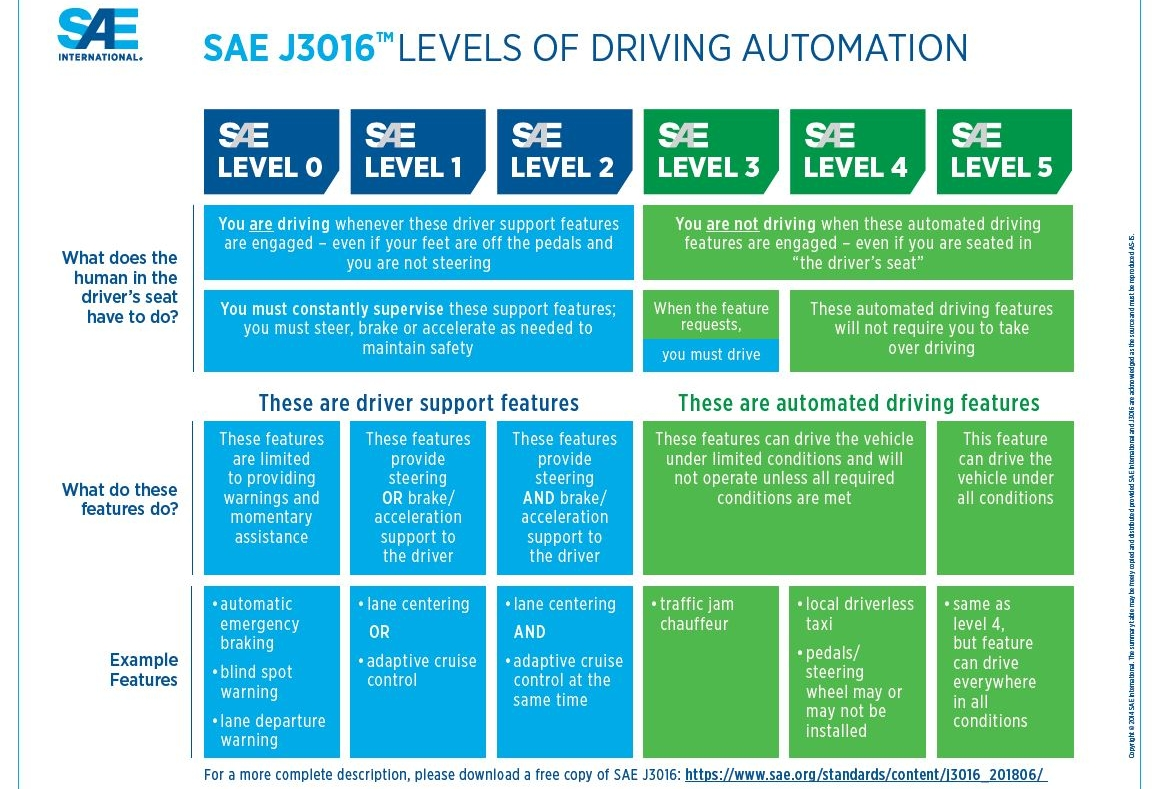
\includegraphics[width=150mm, keepaspectratio]{figures/levels-of-ad.jpg}
    \caption{Levels of driving automation defined in SAE J3016~\cite{j3016b}}
    \label{fig:J3016}
\end{figure}

From level 0 to 2 are automations where the human is still required to fully
monitor the driving environment. Tesla's autopilot is Level 2 which is partial
automation that includes control of steering and both acceleration and
deceleration. From Level 3 the human is not required to monitor the environment.
Full automation, where the driver is not expected to intervene and the vehicle
is able to handle all situations is on Level 5. In order to achieve that level
the autopilot must fully understand the environment.

This is however difficult. The algorithms that we know today are not enough
to achieve understanding of the environment yet. Even Convolutional Neural
Networks (CNNs) are not cabale of understanding deep concepts of the world. CNNs
are mainly used in computer vision and are useful when we want to recognize
patterns that appear anywhere in 2D images. Today we are able to calssify
images, detect and localize objects, segment images to high accuracy,
however this doesn't mean the computer \emph{understands} the scenes.
Furthermore these algorithms are trained specifically: To build a detection
neural network (NN) first a meticulous dataset must be created that tells the
algorithm what must be detected - we call this the ground truth, or training
data set. Then the NN must be trained and optimized until it yields a low error
on the test dataset. We call this Deep Learning due to the fact that the
networks contain millions of parameters that are trained through hundreds of
thousands of iterations. This is not close to what might be general AI.

In this sense we can argue about the meaning of "scene understanding". There is
research going on in the direction of general AI most notably in my opinion by
Yann LeCun the chief at Facebook AI and professsor at NYU, who works a concept
called energy-based models. The Energy-based model that is a form of generative
model allow a mathematical "bounding" or "learning" of a data distribution in
any dimension. Upon prediciton the model tries to generate a possible future for
the current model in time, where the generated future model acts as the
prediciton itself. Generative adversarial networks are a type of these models.
This is in contrast to the other main machine learning approach that is the
discriminative model which is what we use mostly. Perceptrons such as NNs and
CNNs, support vector machines fall into this category, however the distinction
is not clear.

For the purpouse of this thesis hence it is important to define what a system
capabale of understanding scences in driving situations means. The essentials
are the following:
\begin{itemize}
    \item Lane  and path detection
    \item Driveable area detection
    \item Object detection: cars, pedestrians, etc.
    \item Object localization in 3D real world space
    \item Object tracking and identification
    \item Foreign object detection: anything that shouldn't be where it is
    \item Traffic light and sign understanding
    \item Handling occlusion of objects
    \item Pedestrian crossing detection
    \item Knowledge of surroundings and road for example with the help of high
          definition maps
\end{itemize}

In an ideal world, where all cars are autonomous these perceptions would be
enough, however the future of self-driving cars is going to be a transition,
where both humans and machines will drive on the roads. We humans already
account for each other (we try as we can), but self-driving cars will have to
account for us too. We might not be smart but driving on the road sometimes
requires improvization to save a situation and we might need a more general AI.

For the vehicle to understand it's surroundigs first of all it needs sensors.
Each company goes differently about the sensor suite, and it is quite
interesting to examine each solution. This will be discussed in the next
chapter, Related works.

\section{Proposed solution}

In order to develop the proposed system, a sizeable dataset is needed. There are
many datasets available on the internet for car driving. They include object
detections, segmentations, map data, lidar data. Some of the most notable ones
are the nuScenes dataset~\cite{DBLP:journals/corr/abs-1903-11027}, Waymo
dataset~\cite{sun2019scalability} from Google's self-driving car company or the
Cityscapes dataset~\cite{Cordts2016Cityscapes} and more. Each of these datasets are
good, however they are not really helpful for our case.

In order to localize objects in 3D space I use stereo imaging. Each AD system
today employs stereo camera setting because it is a simple and cheap but
accurate way of estimating depth for each pixel in an image. In order to have
the \emph{freedom} to create a custom camera setting I cannot rely on these
datasets. Furthermore, I want to measure the success rate of my detector however
there is no dataset that contains all the necessary information, because in fact
it is not possible to collect everything from the real world.

This is why I choose to use a \emph{simulation} instead to test the system.
Using a simulation gives a huge ammount of freedom. My research work started
in looking for simulators that let me extract data from the simulation in each
frame and let's me create custom world scenario and sensor settings. 

After an extensive research of self-driving car simulators of I found CARLA
Simulator~\cite{Dosovitskiy17} (a
screenshot is seen on \autoref{fig:carla}) to be the most advanced one that is
also opensource. CARLA is a quite mature simulator with an API that
fulfills our requirements.

\begin{figure}[!ht]
    \centering
    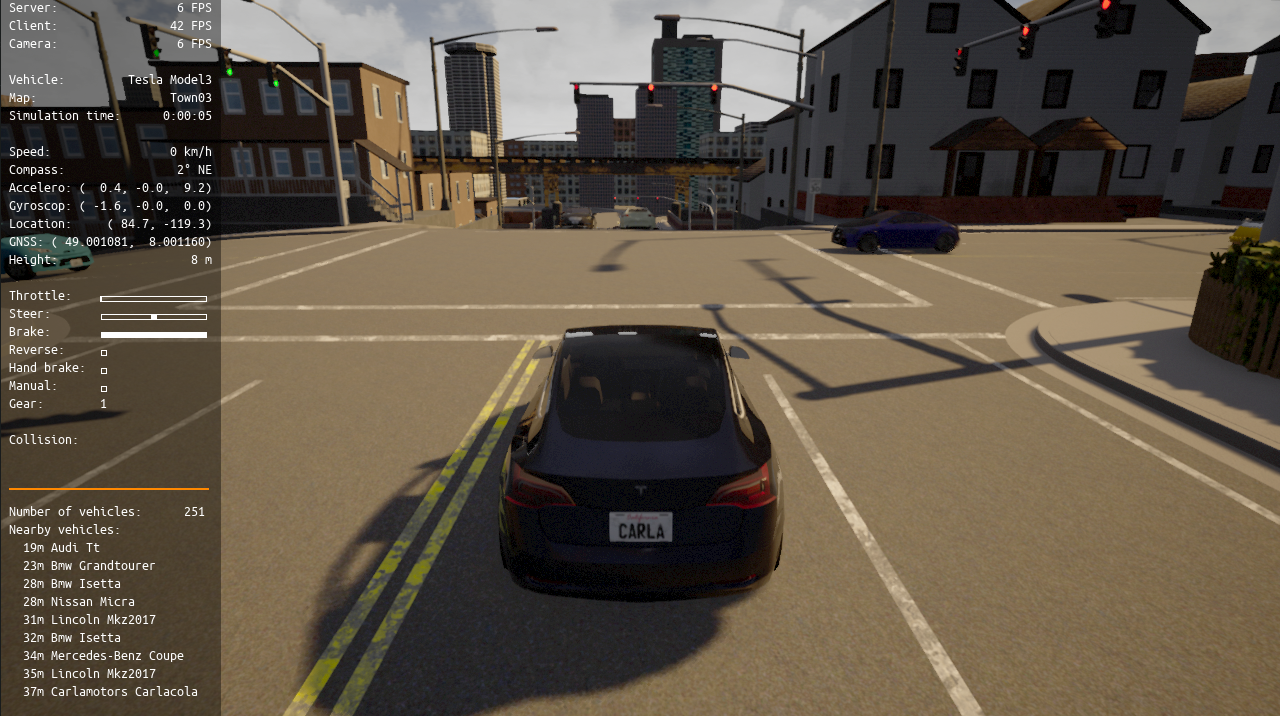
\includegraphics[width=150mm, keepaspectratio]{figures/carla.png}
    \caption{A screenshot from CARLA}
    \label{fig:carla}
\end{figure}

I set up the virtual vehcile with 10 RGB cameras mounted on the roof creating 4
stereo sides as shown on \autoref{fig:3dmodel2}. As the title of the thesis
says, I only used RGB cameras and no other sensors. This is a similar approach
to what Tesla is taking, except for the radar sensors, contrary to almost all
other players in the field who also employ a Lidar sensor for depth data
including MobilEye and Waymo. Lidar data is good for correction, but it is
better if the AI can equally perform using only RGB cameras, since it is a more
general solution that is closer to how we humans percieve the environment.

\begin{figure}[!ht]
    \centering
    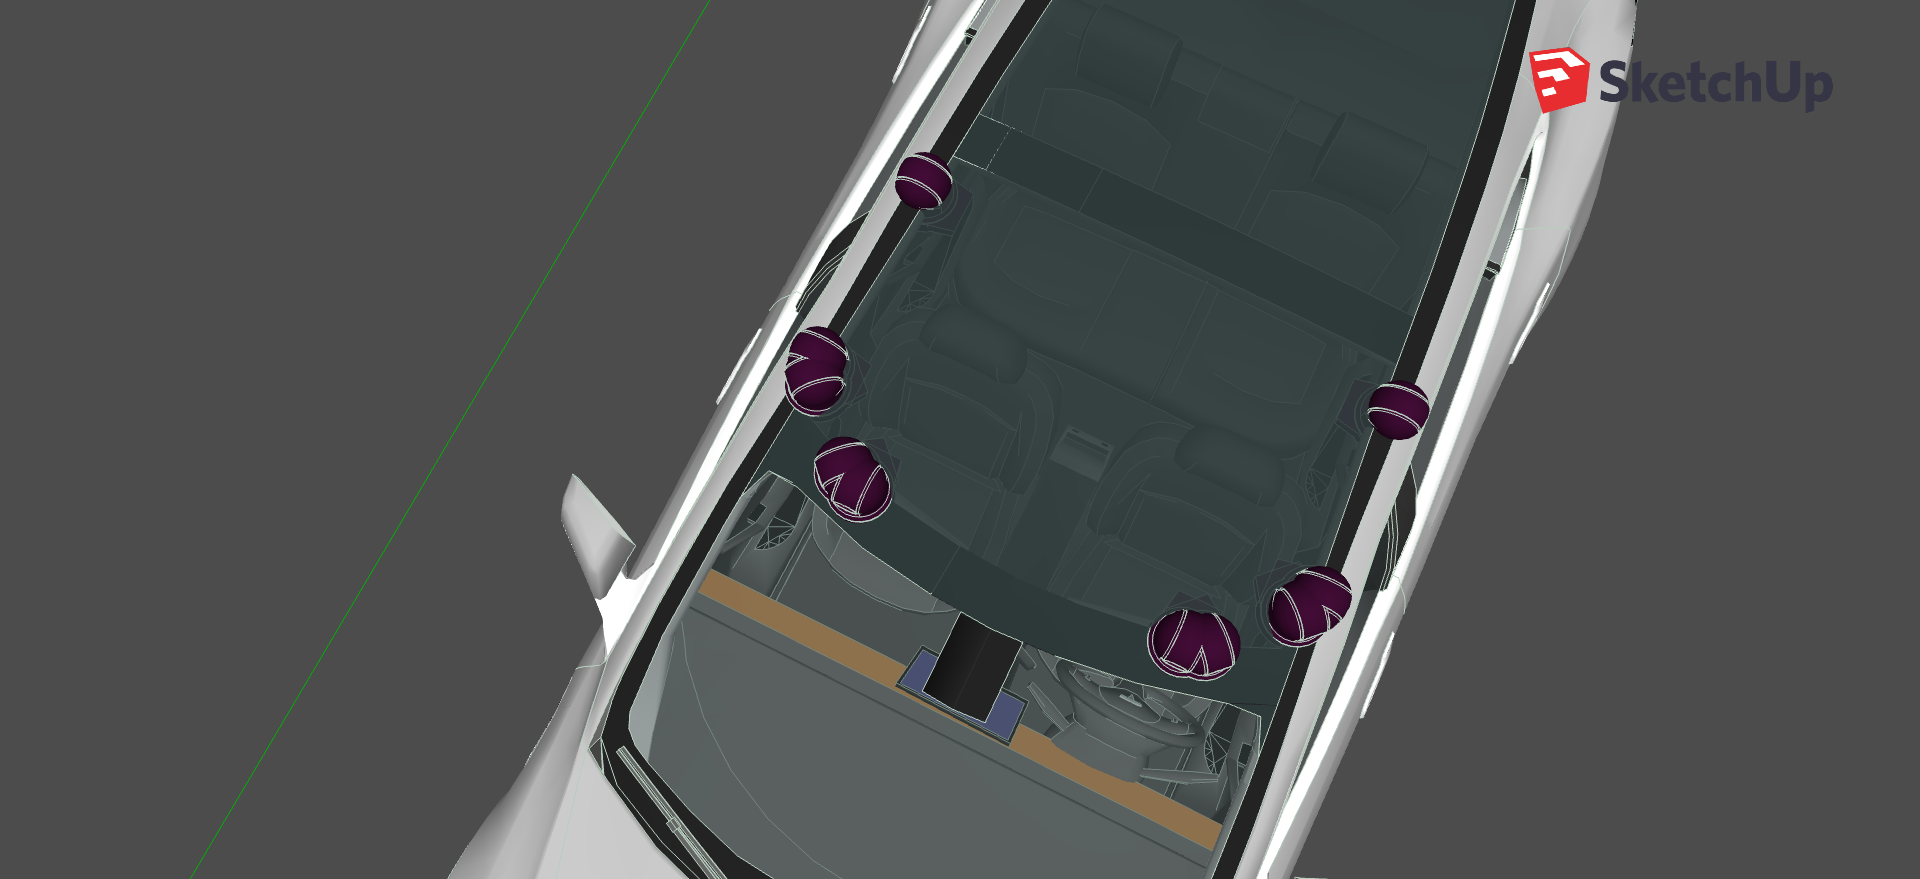
\includegraphics[width=150mm, keepaspectratio]{figures/3dmodel2.png}
    \caption{How the cameras are set up on the roof}
    \label{fig:3dmodel2}
\end{figure}

The detector uses state-of-the-art detection, localization and segmentation model
Detectron2~\cite{wu2019detectron2} a MASK R-CNN conv net model based on Residual
neural networks and Feature Pyramid Networks trained on the COCO~\cite{DBLP:journals/corr/LinMBHPRDZ14} general
dataset.

Finally I develop a 3D webvisualizer that lets us replay the ground truth and
detection log simultaneously and compare the error between the two.

\autoref{fig:flow} depicts this taskflow.

\begin{figure}[!ht]
    \centering
    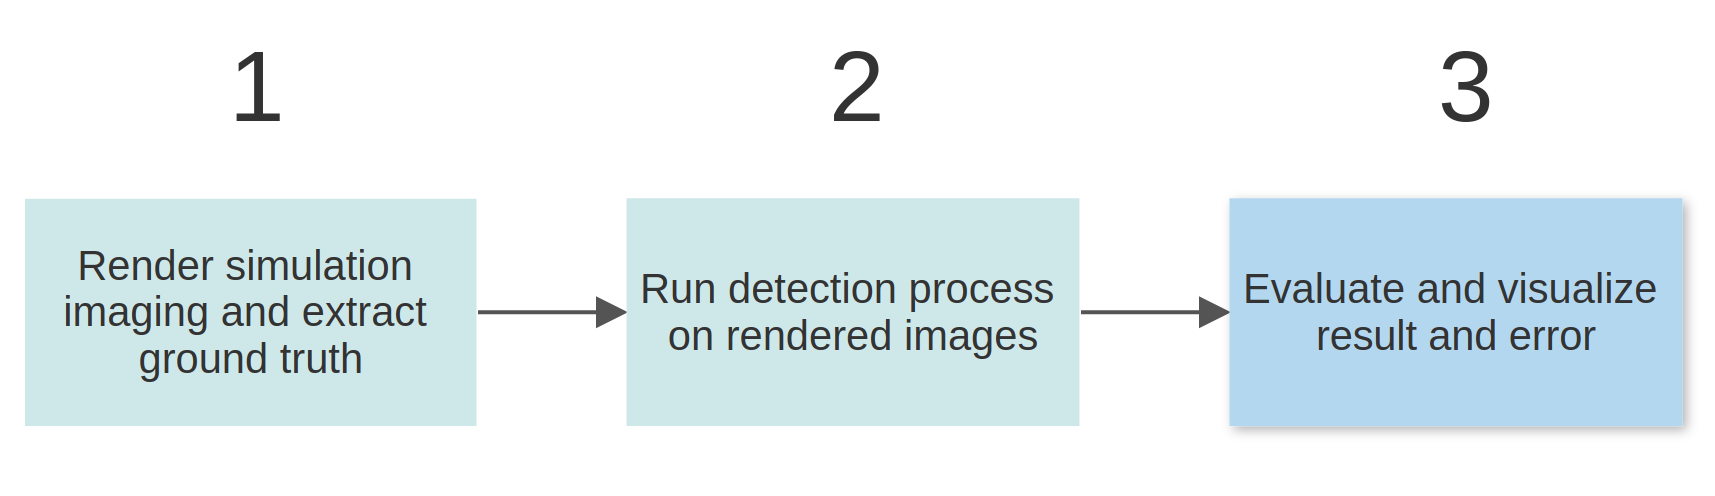
\includegraphics[width=150mm, keepaspectratio]{figures/flowchart.png}
    \caption{Task flow}
    \label{fig:flow}
\end{figure}

\section{Summary of results}

The result is a detector that is capable of localizing vehicles, and pedestrians
on the road up to 100 meters with an accuracy of ~50cm in an angle of 270\degree
centered to the front. The algorithm is written in Python and uses PyTorch, with that on
an NVIDIA Titan X GPU the detector can perform in 2.7FPS for one side, ie. for
two cameras. In an embedded optimized system using C or C++ code this can easily
be improved to even 60FPS creating a real-time system. The code cannot perform
lane detection yet, but that would have been the easier part. The webvisualizer
let's us relplay the simulation frame by frame and see the detection error for
each actor in the scene. It also shows a montage the original, detection and
depthmap. Below, \autoref{fig:webviz1} shows a screenshot of the webvisualizer
in action.

\begin{figure}[!ht]
    \centering
    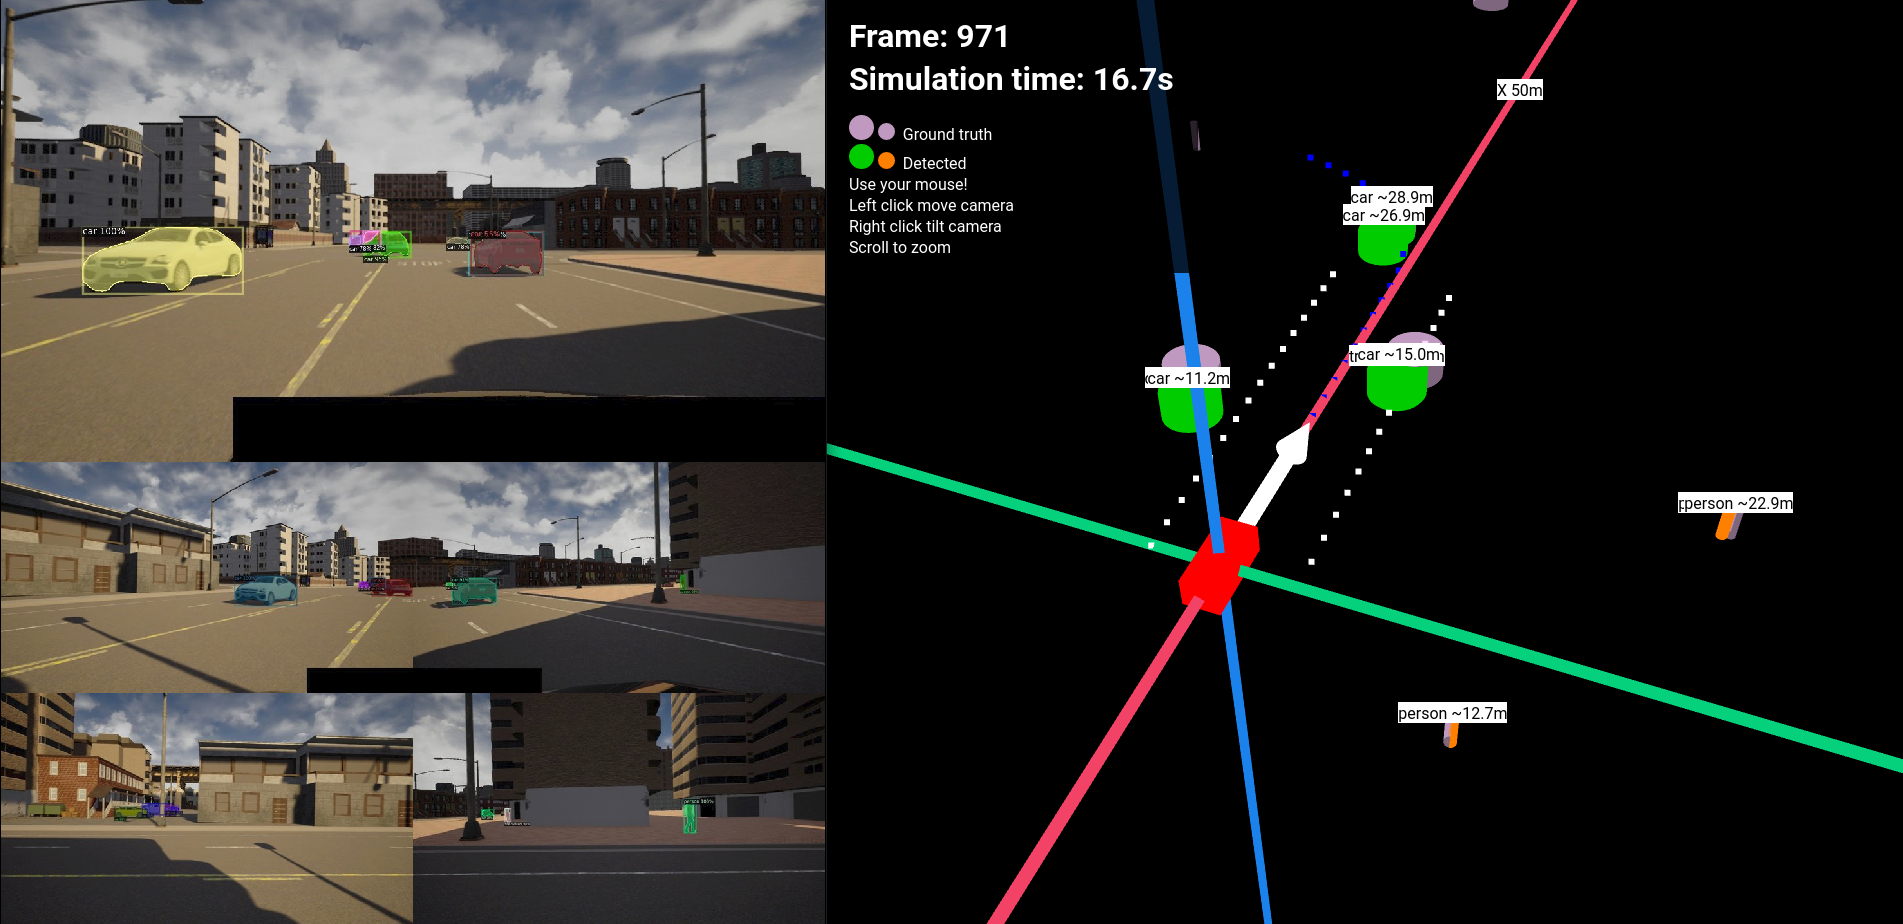
\includegraphics[width=150mm, keepaspectratio]{figures/webviz2.png}
    \caption{3D wevisualizer}
    \label{fig:webviz1}
\end{figure}

All of the code for the thesis, detector, simulator configuration and
webvisualizer is available on \url{https://github.com/najibghadri/msc-thesis}
and you can access the webvisualizer and interactively replay and test
simulations on \url{https://najibghadri.com/msc-thesis/}.


\section{Thesis structure}

In \autoref{chap:sensors} I give an overview of the widely used sensors for
peception in the automotive industry: RGB cameras, radar, Lidar and ultrasonic
sensors. In \autoref{chap:perceptions} I talk about different kinds of
perceptions, state-of-the-art Convolutional Networks and computer vision
algorithms that are useful for our use-case.

In \autoref{chap:relatedwork}, I analyze and compare different self-driving  car
solutions: Tesla and Waymo self-driving cars and MobilEye autopilot. In
\autoref{chap:carlasim}, I introduce CARLA Simulator and some notable features
of it.

In \autoref{chap:assumptions} I define the technical assumptions that I made in
order to simplify the task and the resulting limitations.

\autoref{chap:designimplementation} introduces the Carla simulator details the
design and implementation of the simulator configuration, the detector algorithm
and the webvisualizer.

Then in \autoref{chap:results} I present different measurements and results, and
in \autoref{chap:experimental} I present experimentations that ended up not
being part of the detection. Finally I discuss ways to improve the system in
\autoref{chap:improvement} and close with a conclusion.
%----------------------------------------------------------------------------
\chapter{Sensors}
\label{chap:sensors}
%----------------------------------------------------------------------------

Selecting the right sensors to understand the environment is half the task.
Combining multiple sensors to collect data for further information extraction is
called sensor fusion. In this chapter we are going to detail the most widely
used sensors for scene understanding for autonomous vehicles and compare them. 

Radar, utrasonic and LiDar sensors basically all work the same: emit a wave,
wait until it returns and estimate the distance based on the time difference,
and estimate the speed calculating the frequency shift - this is the Doppler
effect: an increase in frequency corresponds to an object approaching and vice
versa. A visualization is seen on \autoref{fig:sensors}.

\begin{figure}[!ht]
    \centering
    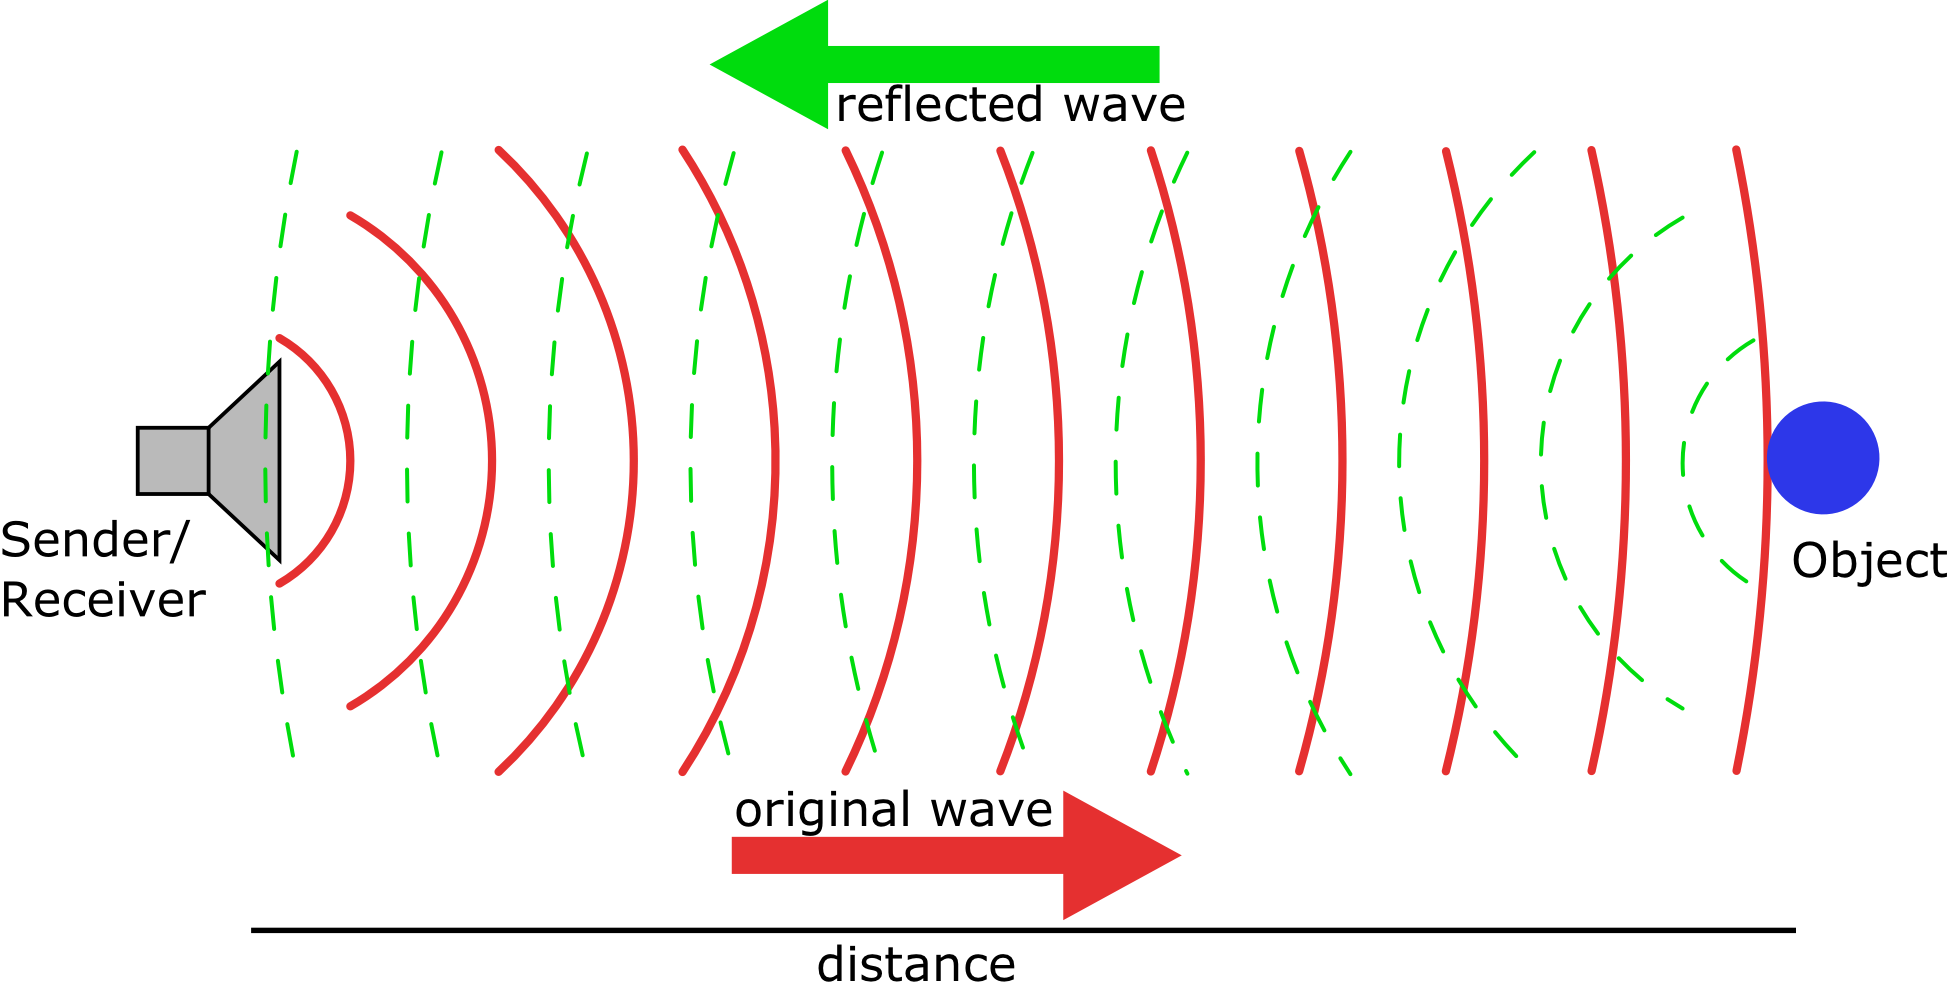
\includegraphics[width=150mm, keepaspectratio]{figures/sensors.png}
    \caption{Sensing object with wave emission and reflection}
    \label{fig:sensors}
\end{figure}

Thus calculating the distance is a simple equation:

\begin{align}
Distance=\frac{Speed\; of\; wavefrom * Time\; of\; Flight}{2}
\end{align}

However they use different waves: Radar works with electromagnetic waves,
ultrasonic sensors work with sound waves and LiDar works with laser light.

\section{Radar}

Radar sensors at the front, rear and sides have become an essential component in
modern production vehicles. Though most frequently used as part of features like
parking assistance and blind-spot detection, they have the capability to detect
objects at much greater range – several hundred meters in fact.

Radar sensors are excellent at detecting objects, but they’re also excellent for
backing up other sensors. For instance, a front-facing camera can’t see through
heavy weather. On the other hand, radar sensors can easily penetrate fog and
snow, and can alert a driver about conditions obscured by poor conditions. Radar
is robust in harsh environments (bad light, bad weather, extreme temperatures).

Automotive radar sensors can be divided into two categories: short-range radar
(SRR), and long-range radar (LRR). The combination of these types of radar
provides valuable data for advanced driver assistance systems.

\textbf{Short-range radar (SRR)}
Short-range radar (SRR): Short-range radars (SRR) use the 24 GHz frequency and
are used for short range applications like blind-spot detection, parking aid or
obstacle detection and collision avoidance. These radars need a steerable
antenna with a large scanning angle, creating a wide field of view. 


\textbf{Long-range radar (LRR)}
Long-range radar (LRR): Long-range radars (LRR) using the 77 GHz band (from
76-81GHz) provide better accuracy and better resolution in a smaller package.
They are used for measuring the distance to, speed of other vehicles and
detecting objects within a wider field of view e.g. for cross traffic alert
systems. Long range applications need directive antennas that provide a higher
resolution within a more limited scanning range. Long-range radar (LRR) systems
provide ranges of 80 m to 200 m or greater.

\section{Ultrasonic}

Ultrasonic (or sonar) sensors like radar, can detect objects in the space around
the car. Ultrasonic sensors are much more inexpensive than radar sensors, but
have a limited effective range of detection. Because they’re effective at short
range, sonar sensors are frequently used for parking assistance features and
anti-collision safety systems. Ultrasonic sensors are also used in robotic
obstacle detection systems, as well as manufacturing technology. In comparison
to infrared sensors in proximity sensing applications, ultrasonic sensors are
not as susceptible to interference of smoke, gas, and other airborne particles
(though the physical components are still affected by variables such as heat),
and they are independent of light conditions. They also work based on reflected
emission. 

Ultrasound signals refer to those above the human hearing range, roughly from 30
to 480 kHz. For ultrasonic sensing, the most widely used range is 40 to 70 kHz.
At 58 kHz, a commonly used frequency, the measurement resolution is one
centimeter, and range is up to 11 meters. At 300 kHz, the resolution can be as
low as one millimeter; however, range suffers at this frequency with a maximum
of about 30 cm.

You can see the sensor suite of Tesla \autoref{fig:teslasensors} from
Tesla Autopilot website \footnote{Tesla autopilot
\url{https://www.tesla.com/autopilot}}.

\begin{figure}[!ht]
    \centering
    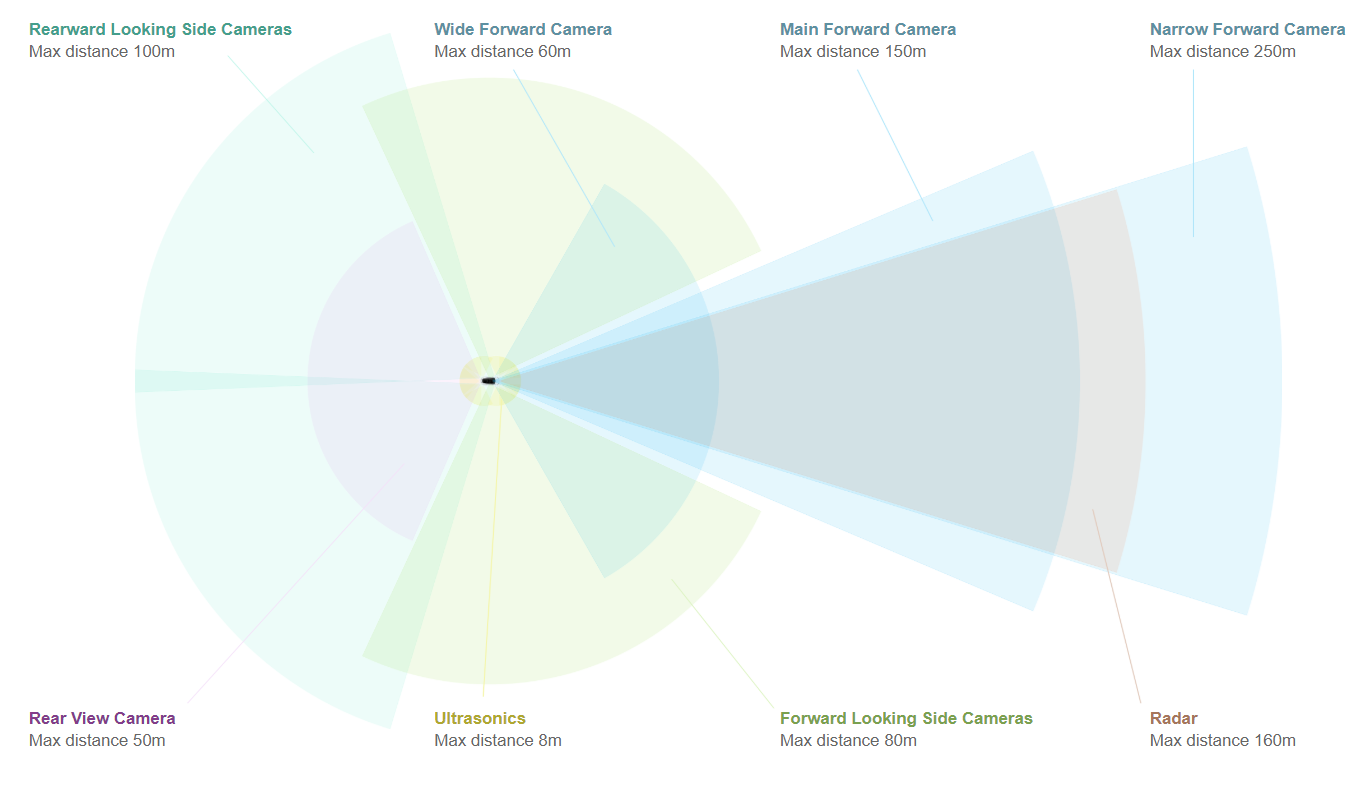
\includegraphics[width=150mm, keepaspectratio]{figures/teslasensors.png}
    \caption{Tesla sensor suite infographic }
    \label{fig:teslasensors}
\end{figure}


\section{LiDAR}

As Radar is to radio waves, and sonar is to sound, LiDAR (Light Detection and
Ranging) uses lasers to determine distance to objects. Lidar sometimes is called
3D laser scanning. It does this by spinning a laser across its field of view and
measuring the individual distances to each point that the laser detects. This
creates an extremely accurate (within 2 centimeters) 3D scan of the world around
the car.

The principle behind LiDAR is really quite simple. Shine a small light at a
surface and measure the time difference it takes to return to its source. The
equipment required to measure this needs to operate extremely fast. The LiDAR
instrument fires rapid pulses of laser light at a surface, some at up to 150,000
pulses per second. A sensor on the instrument measures the amount of time it
takes for each pulse to bounce back. Light moves at a constant and known speed
so the LiDAR instrument can calculate the distance between itself and the target
with high accuracy. By repeating this in quick succession the insturment builds
up a complex 'map' of the surface it is measuring.

The three most common currently used or explored wavelengths for automotive
lidar are 905 nm, 940 nm and 1550 nm, each with its own advantages and
drawbacks.

Lidar sensors are able to paint a detailed 3D point cloud of their environment
from the signals that bounce back instantaneously. It provides shape and depth
to surrounding cars and pedestrians as well as the road geography. And, like
radar, it works just as well in low-light conditions.

You can see how a lidar sensor from Luminar\footnote{Luminar
\url{https://www.luminartech.com/}} reconstructs the environment in
\autoref{fig:luminar}.

\begin{figure}[!ht]
    \centering
    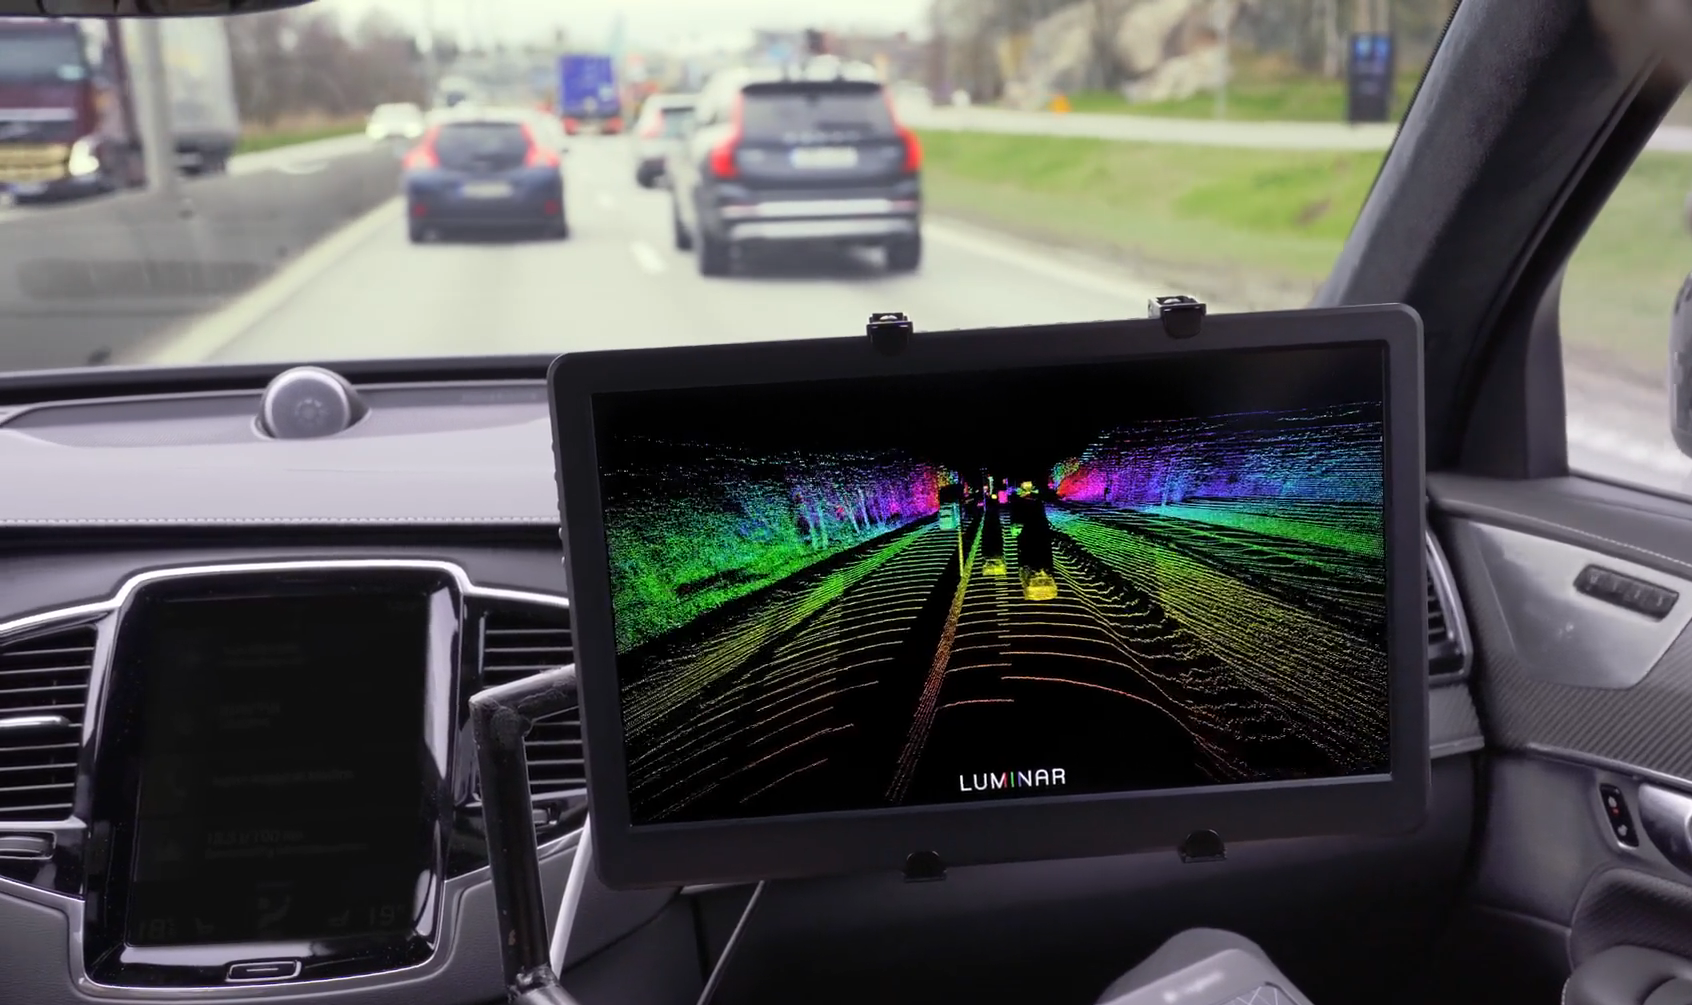
\includegraphics[width=150mm, keepaspectratio]{figures/luminar.png}
    \caption{Luminar LiDAR in action}
    \label{fig:luminar}
\end{figure}


Currently, LiDAR units are big, and fairly expensive - as much as 10 times
the cost of camera and radar — and have a more limited range. You will most
often see them mounted on Mapping Vehicles, but as the technology becomes
cheaper, we might see them on trucks and high-end cars in the near future.

\section{RGB Cameras}

Cameras are the essential sensors for self-driving cars. Most imaging sensors
are sensitive from about 350 nm to 1000 nm wavelengths. The most common types of
sensors for cameras are CCD (charged coupled device) and CMOS (complementary
metal–oxide–semiconductor). The main difference between CCD and CMOS is how they
transfer the charge out of the pixel and into the camera’s electronics.

CCD-based image sensors currently offer the best available image quality, and
are capable of high resolutionsm making them the prevalent technology for still
cameras and camcorders.

An important aspect of cameras is the camera model that describes how points of
the world translate to pixels in the image. That is going to be essential when
we want to apply the inverse projection to determine the world-position of
objects in the picture. I will talk about this in the next chapter. 


\section{GPS \& WPS}

The Global Positioning System is the perfect example of how sensor
technology grows smaller and more ubiquitous over time. Originally introduced
for military applications in 1974, GPS probes today can be found in cameras,
watches, key fobs, and of course, the smartphone in your pocket.

The lesser-known WPS stands for Wi-Fi Positioning System, which operates
similarly. When a probe detects satellites (GPS) or Wi-Fi networks (WPS), it can
determine the distance between itself and each of those items to render a
latitude and longitude. The more devices a GPS/WPS probe can detect, the more
accurate the results. On average, GPS is only accurate to around 20 meters.

For WPS the most common and widespread localization technique is based on
measuring the intensity of the received signal, and the method of
"fingerprinting". Typical parameters useful to geolocate the wireless access
point include its SSID and MAC address. The accuracy depends on the number of
nearby access points whose positions have been entered into the database. The
Wi-Fi hotspot database gets filled by correlating mobile device GPS location
data with Wi-Fi hotspot MAC addresses.
%----------------------------------------------------------------------------
\chapter{Computer vision}
\label{chap:perceptions}
%----------------------------------------------------------------------------

After collecting data from the sensors we choose we need to implement the right
algorithms to extract information from the sensor data. In this chapter I start
with explaining basics of computer vision and then move on to advanced
convolutional neural netowrks that will help our goal.

Computer Vision, often abbreviated as CV, is defined as a field of study that
seeks to develop techniques to help computers “see” and understand the content
of digital images such as photographs and videos.

The problem of computer vision appears simple because it is trivially solved by
people, even babies. Nevertheless, it largely remains an unsolved
problem based both on the limited understanding of biological vision and because
of the complexity of vision perception in a dynamic and nearly infinitely
varying physical world.

\section{Challenges in Computer Vision}
Image Classification is considered to be the most basic application of computer
vision. Rest of the other developments in computer vision are achieved by making
small enhancements on top of this. In real life, every time we, humans open our
eyes, we unconsciously classify and detect objects.

Since it is intuitive for us, we fail to appreciate the key challenges involved
when we try to design systems similar to our eye. Some challenges for computers are:

\begin{itemize}
    \item Variations in viewpoint
    \item Difference in illumination
    \item Hidden parts of images, occulsion
    \item Background Clutter
\end{itemize}

\section{Traditional approaches}

Various techniques, other than deep learning are available enhancing computer
vision. Though, they work well for simpler problems, but as the data become huge
and the task becomes complex, they are no substitute for deep CNNs. Let’s
briefly discuss two simple approaches.

\subsection{KNN (K-Nearest Neighbours)}

In the KNN algorithm each image is matched with all images in training data. The
top K with minimum distances are selected. The majority class of those top K is
predicted as output class of the image. Various distance metrics can be used
like L1 distance (sum of absolute distance), L2 distance (sum of squares), etc.
However KNN performs poorly - qute expectedly - they have a high error rate on
complex images, because all they do is compare pixel values among other images,
without any use of image patterns.

\subsection{Linear Classifiers}

They use a parametric approach where each pixel value is considered as a
parameter. It’s like a weighted sum of the pixel values with the dimension of
the weights matrix depending on the number of outcomes. Intuitively, we can
understand this in terms of a template. The weighted sum of pixels forms a
template image which is matched with every image. This will also face difficulty
in overcoming the challenges discussed in earlier as it is difficult to design a
single template for all the different cases.

\section{Convolutional Neural Networks}

Visual recognition tasks such as image classification, localization, and
detection are key components of Computer vision. However these are not possible
to achieve with traditional vision.

Recent developments in neural networks and deep learning approaches have greatly
advanced the performance of these state-of-the-art visual recognition systems.

Neural networks are the basis of deep learning methods. They are made up of
multiple layers, each layer containing multiple perceptrons. Layers can be
fully-connected or sparsely if possible, providing some performance benefits.
Each perceptron is an activation function whose input is the weighted output of
perceptrons from previous layers, and the function is usually a sigmoid
function. A neural networks first layer is the input layer and the last layer is
the output, which could be an array of perceptron where only one yields a high
output creating a classifier. Layer in-between are called hidden layers and it
is up to design and experimentation the determine what is the right
configuration of hidden layers.

\begin{figure}[!ht]
    \centering
    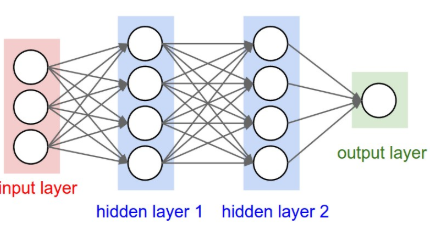
\includegraphics[width=80mm, keepaspectratio]{figures/nn.png}
    \caption{Neural network visualization. Image taken from CS231N Notes}
    \label{fig:convnet}
\end{figure}

Neural Networks (NN) are good at classifying different patterns recieved in the
input layers however they are not sufficient for even image classification,
because in one part the number of inputs is way to high. Consider a high
resolution image with $1000\times 1000\times 3$ pixels, then the NN has 3million input
parameters to process. This takes a long time and too much computational power.

Secondly the neural network architecture in itself is not a
general-enough solution (if you think about it, it is similar to a linear
classifier or a KNN).

Convolutional Neural Network (CNNs) however solve image classification and more.
A CNN is able to capture the spatial features in an image through the
application of relevant filters. The architecture performs a better fitting to
an image dataset due to the reduction in the number of parameters involved and
reusability of weights.


There is material on the internet in abundance about how convolutional neural
networks work, and I have read many of them, but the one I recommend most is the
Stanford course CS231N\footnote{ Stanford CV course CS231N
\url{https://cs231n.github.io/}}. 

The general architecture of CNN is similar to a cone, where the first layer is
the widest and each layer first convolves multiple filters (which in the
beginning of the CNN correspond to edges and corners) applying ReLU (rectifier,
non-linearity function) then it downsizes the input which is called the max
pooling. This repeated over and over in the end results in a small tensor
which can \emph{then} be fed to the fully-connected (FC) layers (i.e. a neural network)
which acts as the classifier.

Why is this the winner architecture? Because if you think about it the neural
network in the end only has to vote for the presence of the right features in roughly
the right image position, not for each pixel. A visualization of a
CNN's architecture can be seen in \autoref{fig:convnet}.

\begin{figure}[!ht]
    \centering
    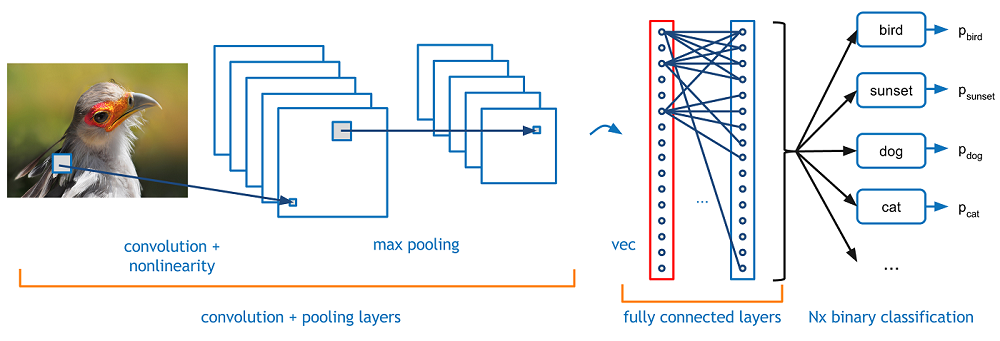
\includegraphics[width=150mm, keepaspectratio]{figures/convnet.png}
    \caption{Architecture of a CNN}
    \label{fig:convnet}
\end{figure}

\begin{figure}[!ht]
    \centering
    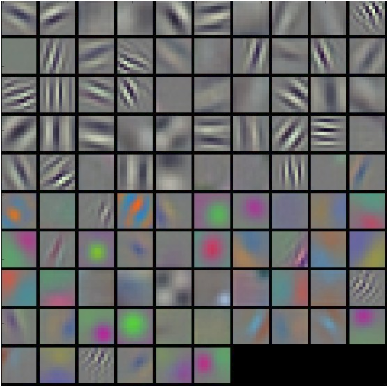
\includegraphics[width=60mm, keepaspectratio]{figures/filters.png}
    \caption{A visualization of the features learned in the first convnet layer in AlexNet~\cite{NIPS2012_4824}. AlexNet was a CNN which revolutionized the field of Deep Learning, and is built from conv layers, max-pooling layers and FC layers. Image taken from CS231N notes.}
    \label{fig:filters}
\end{figure}

There are various architectures that have emerged each incrementally improving on the previous ones:
LeNet~\cite{Lecun98gradient-basedlearning} - the work of Yann LeCun himself,
AlexNet~\cite{NIPS2012_4824}
VGGNet~\cite{DBLP:journals/corr/SimonyanZ14a}
GoogLeNet~\cite{DBLP:journals/corr/SzegedyLJSRAEVR14}
ResNet~\cite{DBLP:journals/corr/HeZRS15}

\subsection{Deep Learning}
Deep learning referes to the procedure of training neural networks and
convolutional neural networks to perform the task at hand accurately. During
deep learning first a dataset is created with training images coupled with
"ground truth" data that is the required prediction for each image. The neural
networks are then fed with the images in batches for a certain number of
iterations - epochs. The weights of the neural network and the filters are
adjusted with the loss function that comes from calculating the error of the
current prediction and the ground truth for each image. This error is then
"backpropagated" which is just another way of saying it is multiplied with the
derivative of each weight in the network and subtracted from it. For filters this means
"filtering filters", so only those filters will stay in the convnet which
resulted in a non-zero gradient in the neural network.

\section{Detection, Classification and Segmentation}
\subsection{Image Classification}

\subsection{Object Detection, Localization}
    (AlexNet, LeNet, VGG)
    R-CNN, Fast, Faster
    YOLO
\subsection{Segmentation}
Segmentation Networks
\subsection{Instance Segmentation}
Mask R-CNN - Detectron2
Yolact
Yolact++
\section{Tracking}
others
SORT
Deep Sort
\section{Bounding box detection and orientation}

\section{Key point detection}

\section{Voxelization}
PointNet
VoxelNet
\section{Lane and road detection}
Traditional way
Road detection
Driveable Road
Lane detection: sliding window, curve fit
\section{3D vision}
Camera model and Calibration
3D reconstruction
Stereo vision
Depth estimation
\section{Datasets}
Datasets - KITTI, MARS, COCO, Waymo, nuScenes










%----------------------------------------------------------------------------
\chapter{Related work}
%----------------------------------------------------------------------------

A bevezető tartalmazza a diplomaterv-kiírás elemzését, történelmi előzményeit, 
a feladat indokoltságát (a motiváció leírását), az eddigi megoldásokat, 
és ennek tükrében a hallgató megoldásának összefoglalását.

A bevezető szokás szerint a diplomaterv felépítésével záródik, 
azaz annak rövid leírásával, hogy melyik fejezet mivel foglalkozik.

%----------------------------------------------------------------------------
\chapter{CARLA Simulator}
\label{chap:carlasim}
%----------------------------------------------------------------------------

CARLA's mission is to create a simulator that can simulate sufficient-enough
real-world traffic scenarios so that it is more accessible for researchers like
myself to research, develop and test computer vision algorithms for
self-driving car. 

CARLA~\cite{Dosovitskiy17} is an open-source simulator for autonomous driving
research. It is written in C++ and provides an accessible Python API to
control the simulaton execution. It has been developed from the ground
up to support development, training, and validation of autonomous driving
systems. In addition to open-source code and protocols, CARLA provides open
digital assets (urban layouts, buildings, vehicles) that were created for this
purpose and can be used freely. The simulation platform supports flexible
specification of sensor suites, environmental conditions, full control of all
static and dynamic actors, maps generation and much more. It is developed by the
Barcelonian university UAB's computer vision CVC Lab and supported by companies
such as Intel, Toyota, GM and others. The repository for the project is at
\url{https://github.com/carla-simulator}

It provides scalability via a server multi-client architecture: multiple clients
in the same or in different nodes can control different actors. Carla exposes a
powerful API that allows users to control all aspects related to the simulation,
including traffic generation, pedestrian behaviors, weathers, sensors, and much
more. Users can configure diverse sensor suites including LiDARs, multiple
cameras, depth sensors and GPS among others. Users can easily create their own
maps following the OpenDrive standard via tools like RoadRunner. Furthermore it
provides integration with ROS\footnote{Robot Operating System (ROS)
\url{https://www.ros.org/}} via their ROS-bridge

I used CARLA 9.8.0 in the project that was the latest at the time (2020 March
09). Carla has a primary support for Linux so I could run it easly on Ubuntu. It
requires a decent GPU otherwise the simulation is going to be slow.

It's important to mind the coordinate system used in Carla, because later when
we will extract data the axes must be mapped to the correct data points. Since
Carla is built with Unreal Engine \footnote{Unreal Engine
\url{https://www.unrealengine.com/}} it uses the coordinate system as in
\autoref{fig:carlacoords}: X coordinate is to the front of the ego actor, Y is to the
right of ego and Z is to the top.

\begin{figure}[!ht]
  \centering
  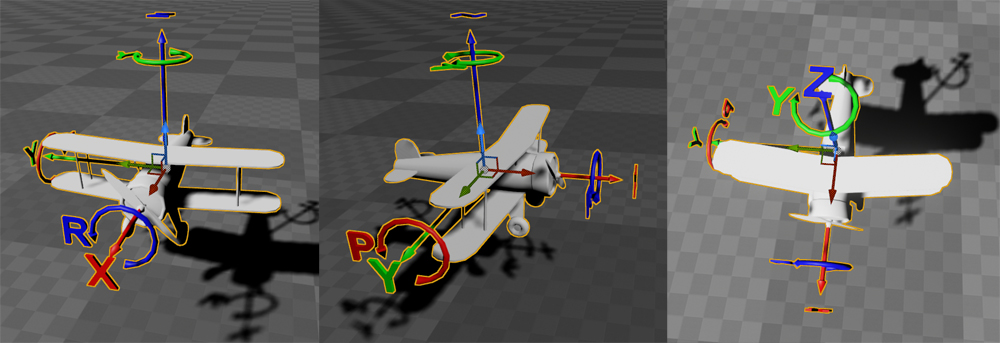
\includegraphics[width=150mm, keepaspectratio]{figures/carlacoords.jpg}
  \caption{Carla coordinate system}
  \label{fig:carlacoords}
\end{figure}


\section{Is a simulation enough?}
I believe the future of self-driving car research and development is in part
with simulations and in part with real-world training as well. To develop a
self-driving AI from ground up it is certainly advisable to first develop and
test the algorithms in a simulation. 

In order to create simulations that are rich and different Carla provides a
large variety of actors and maps. The traffic manager can also be parametrized
to control how pedestrians and vehicles move: their speed, minimum distance, and
even "aggressivity" towards each other, which means how willing are
they to collide instead of waiting until the actor in front moves away. This is
actually useful as it helps unlock possible traffic deadlocks. The latest
CARLA provides 8 maps but in newer versions they will be adding new maps. You
can see a screenshot of each rendering in the 6 maps I used in
\autoref{fig:maps}.

\begin{figure}[!ht]
  \centering
  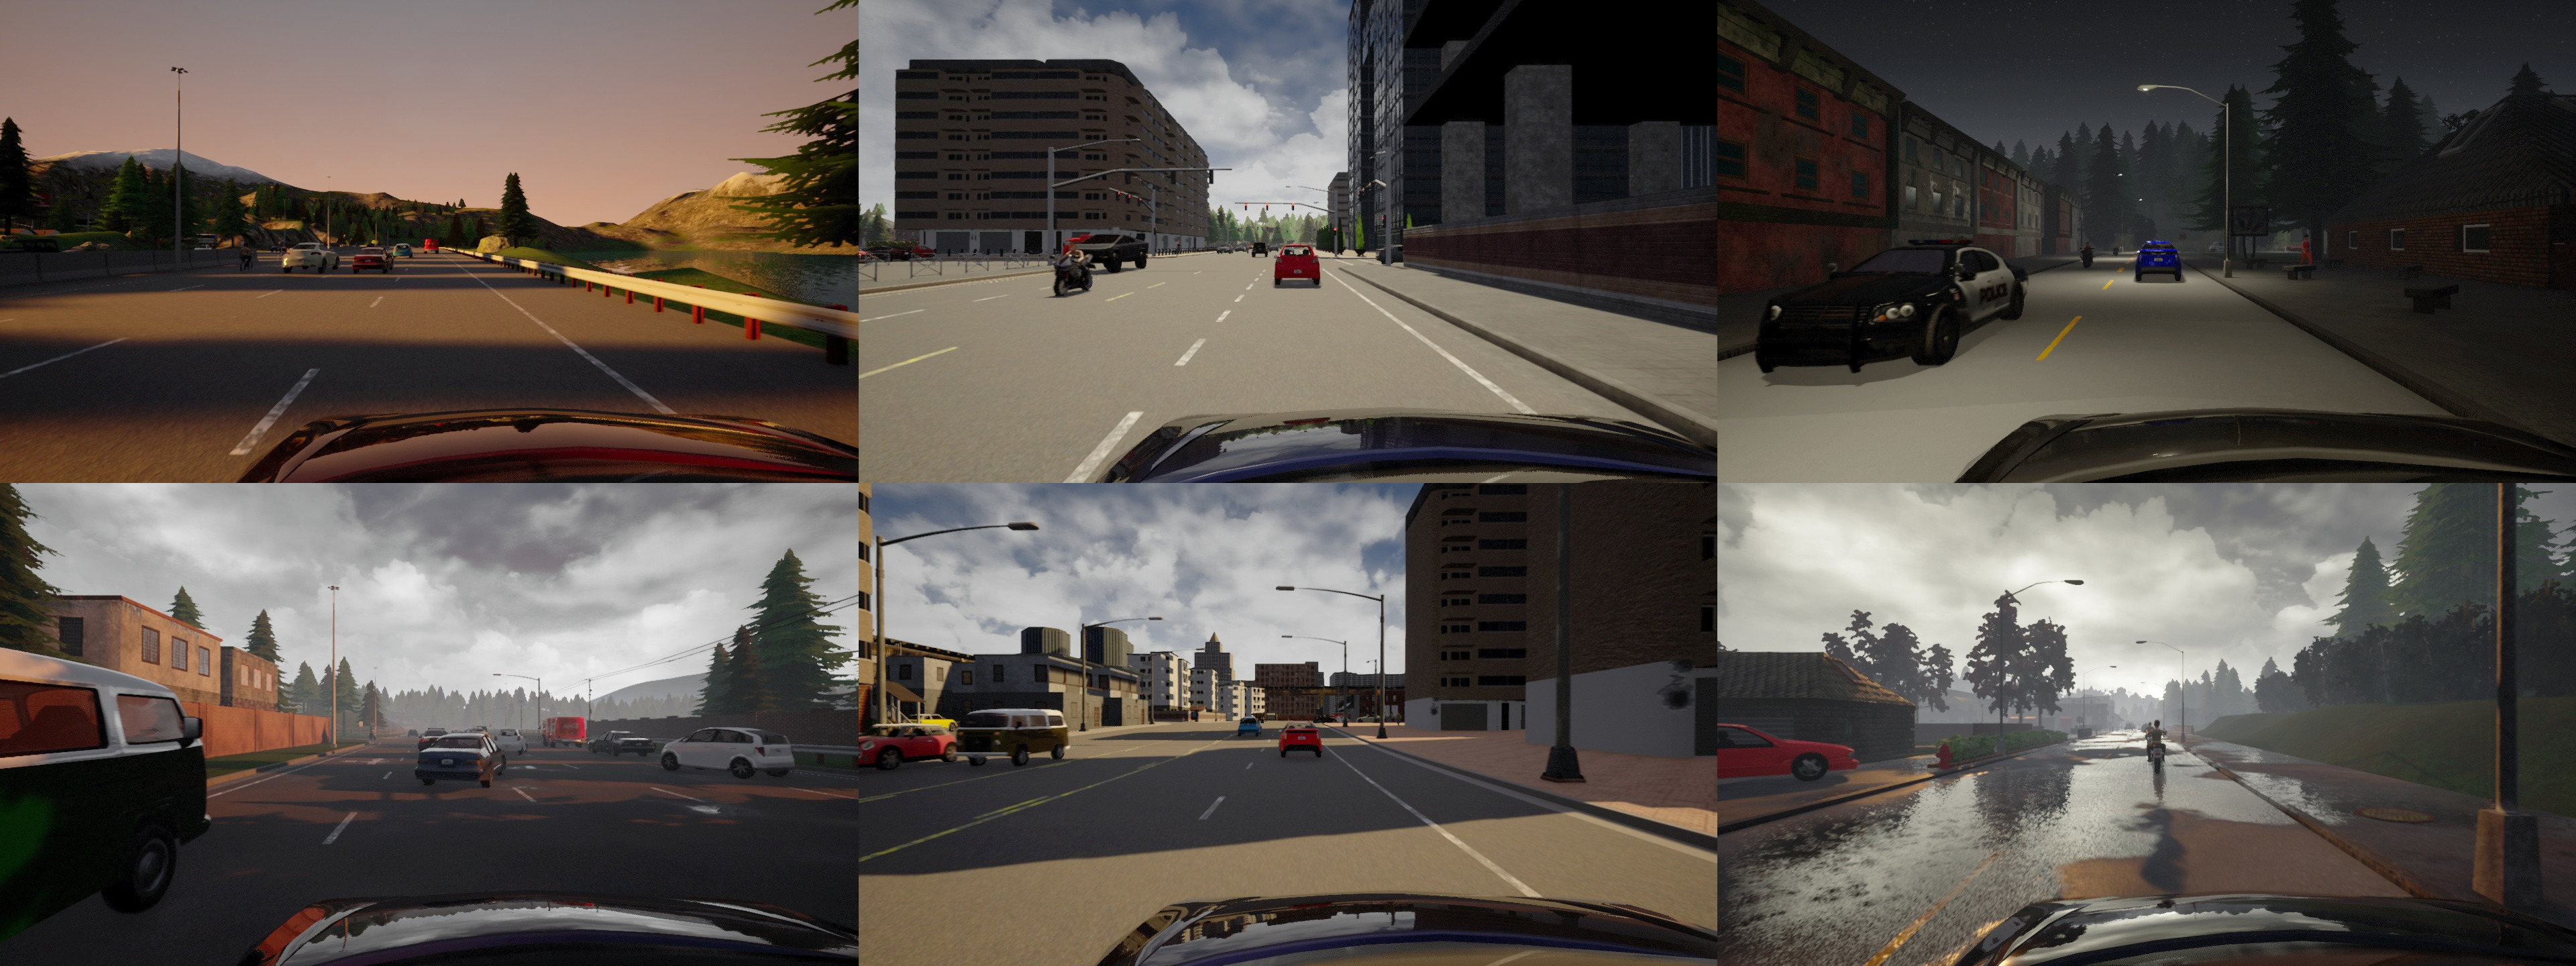
\includegraphics[width=150mm, keepaspectratio]{figures/maps.jpg}
  \caption{Variety of maps in Carla}
  \label{fig:maps}
\end{figure}

A simulation obviously can't return the variety and exact nature of scenarios
that happen in \emph{nature}. However I believe they are sufficient for testing
an entry-level self-driving system and that with the use of simulations a
company can lower the costs of development. The rise of simulators itself shows
there is a need for the market.

\section{CARLA Simulation sensors}

The Carla simulator's API support a wide range of sensors: RGB Cameras, LiDAR,
Radar, GPS, gyroscope, accelerometer, compass and more. These are easy to
use, If you are interested I recommend reading the sensors reference in their
documentation \footnote{CARLA sensors reference
\url{https://carla.readthedocs.io/en/latest/ref_sensors/}}

Carla also provides miscellaneous sensors that help collecting ground-truth data
for deep learning applications. This includes semantic segmentation camera,
depthmap camera and other simple ones such as collision detector as seen in \autoref{fig:carlaseg}.

\begin{figure}[!ht]
  \centering
  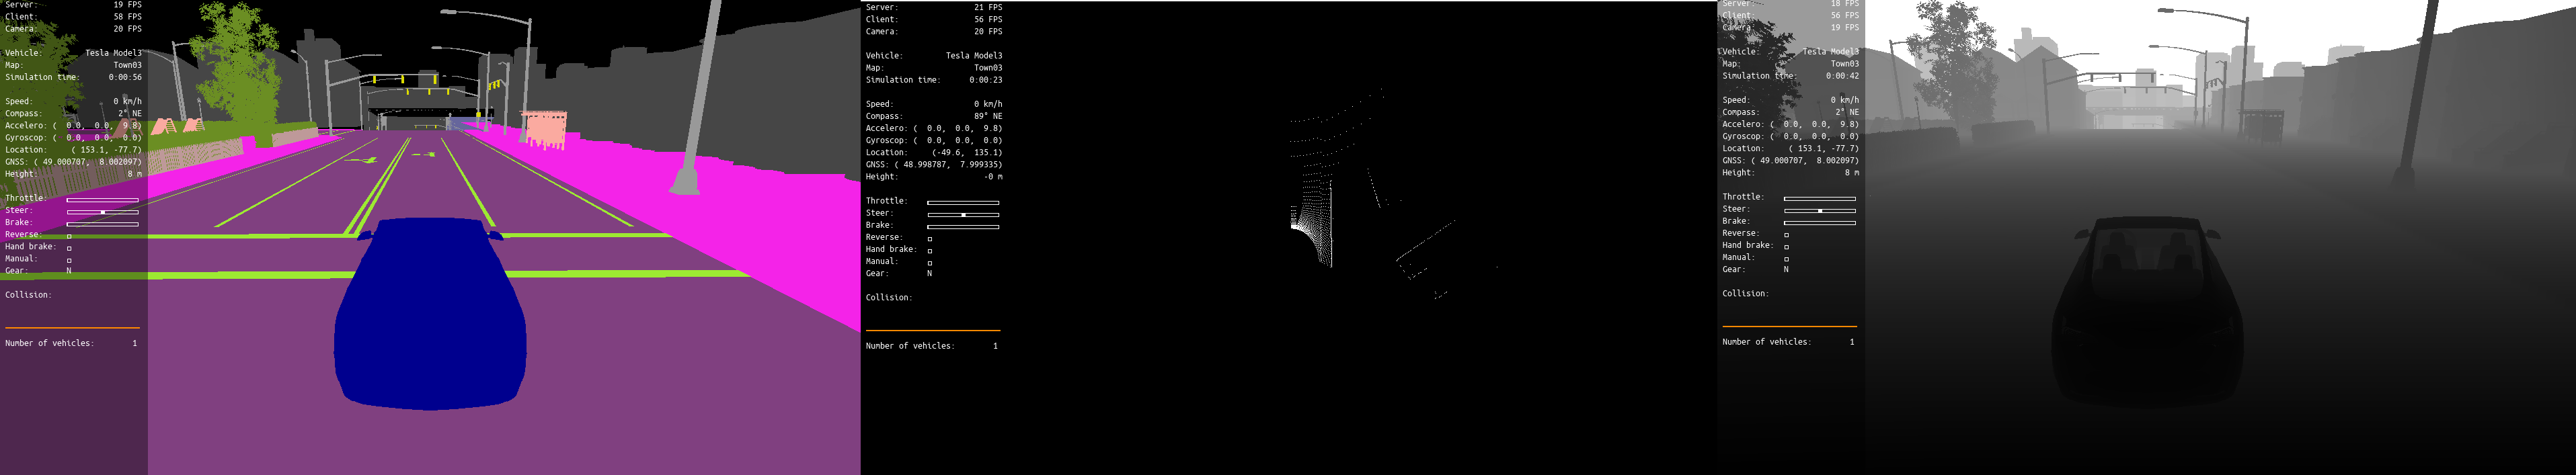
\includegraphics[width=150mm, keepaspectratio]{figures/carlaseg.png}
  \caption{Different sensors and cameras in Carla (semantic segmentation, LiDAR, depthmap)}
  \label{fig:carlaseg}
\end{figure}

\subsection{Other simulators}

There are a couple of other dedicated projects for simulators. There is
Deepdrive from Voyage auto\footnote{Deepdrive Voyage
\url{https://deepdrive.voyage.auto/}}, an American AD supplier, NVIDIA has a
project going on called Drive Constellation\footnote{NVIDIA Drive Constellation
\url{https://developer.nvidia.com/drive/drive-constellation}} which is said to
be advanced but is not opensource. Nvidia provides Harware In the Loop
simulation for Drive Constellation which is an even more advanced simulation
infrastructure that allows for testing the systems real-timeness. There is
another project called RFPro\footnote{RFPro \url{http://www.rfpro.com/}}.
However these are either not opensource or not mature enough. CARLA
Simulator~\cite{Dosovitskiy17} was by far the best one
for my case.
%----------------------------------------------------------------------------
\chapter{Assumptions made and limitations}
%----------------------------------------------------------------------------

A bevezető tartalmazza a diplomaterv-kiírás elemzését, történelmi előzményeit, 
a feladat indokoltságát (a motiváció leírását), az eddigi megoldásokat, 
és ennek tükrében a hallgató megoldásának összefoglalását.

A bevezető szokás szerint a diplomaterv felépítésével záródik, 
azaz annak rövid leírásával, hogy melyik fejezet mivel foglalkozik.

%----------------------------------------------------------------------------
\chapter{Design and implementation}
\label{chap:designimplementation}
%----------------------------------------------------------------------------

Let's recap the task flow of the task I described in the Introduction: After
configuring the simulator with the designed camera setting I render multiple
traffic scenarios in different maps provided by CARLA while extracting all
necessary information into a log file to later compare the detection log with


\begin{figure}[!ht]
    \centering
    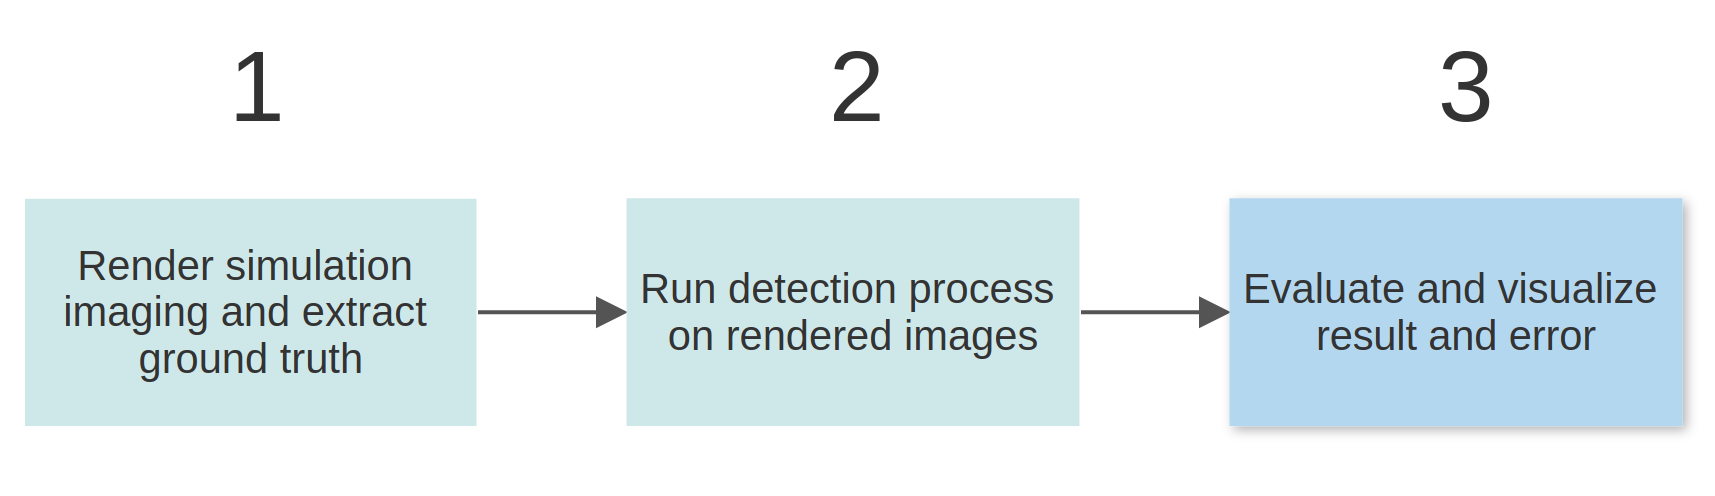
\includegraphics[width=150mm, keepaspectratio]{figures/flowchart.png}
    \caption{Task flow}
    \label{fig:flow2}
\end{figure}


\section{Tools used}

Soon it became obvious that Linux operating system is the right tool to use
for development. I have been using Ubuntu before this project as well so I was
already familiar with everything. The main IDE I used throughout the project is
Visual Studio Code, which thanks to it's openness and community has many useful
extensions that helped me develop in fact every part of the thesis: Python,
Nodejs and Javascript for the webvisualizer and finally LaTeX and ofcourse git
support.

I also used Conda which is I think an essential tool when you want to develop ML
and AI projects with Python. Conda makes it easy to create and use separate
Python environments. This is important because different implementations of
algorithms require different versions of the same packages thus it keeps a clean
separation. The drawback is that consecuently it requires an excessive ammount
of hard-drive space.

Upon developing the algorithm and experimenting with it I used Jupyter Notebook
which is a Python runtime on top of the bare one and a web-based IDE at the same
time. With Jupyter Notebook it is easy to change and re run the code thanks
to it's "kernel" system, which keeps the value of variable and imported packages
between executions.

For the GPU-intensive tasks such as simulation and convnet calculations in the
detector I was provided with a remote Titan X GPU\footnote{ Titan X GPU
    \url{https://www.nvidia.com/en-us/geforce/products/10series/titan-x-pascal/}} by
my university.

\section{Choosing the sensor suite}

Mounting cameras around the vehicle to have an all around vision is an essential
design strategy, as we have seen in the work of other companies in
\autoref{chap:relatedwork}. However we will need to determine depth as well. I
decided to use only cameras in a stereoscopic structure to create 4 stereo sides
around the vehicle. The following image shows the design setting with field of
views visualized in \autoref{fig:3dmodel3}.

\begin{figure}[!ht]
    \centering
    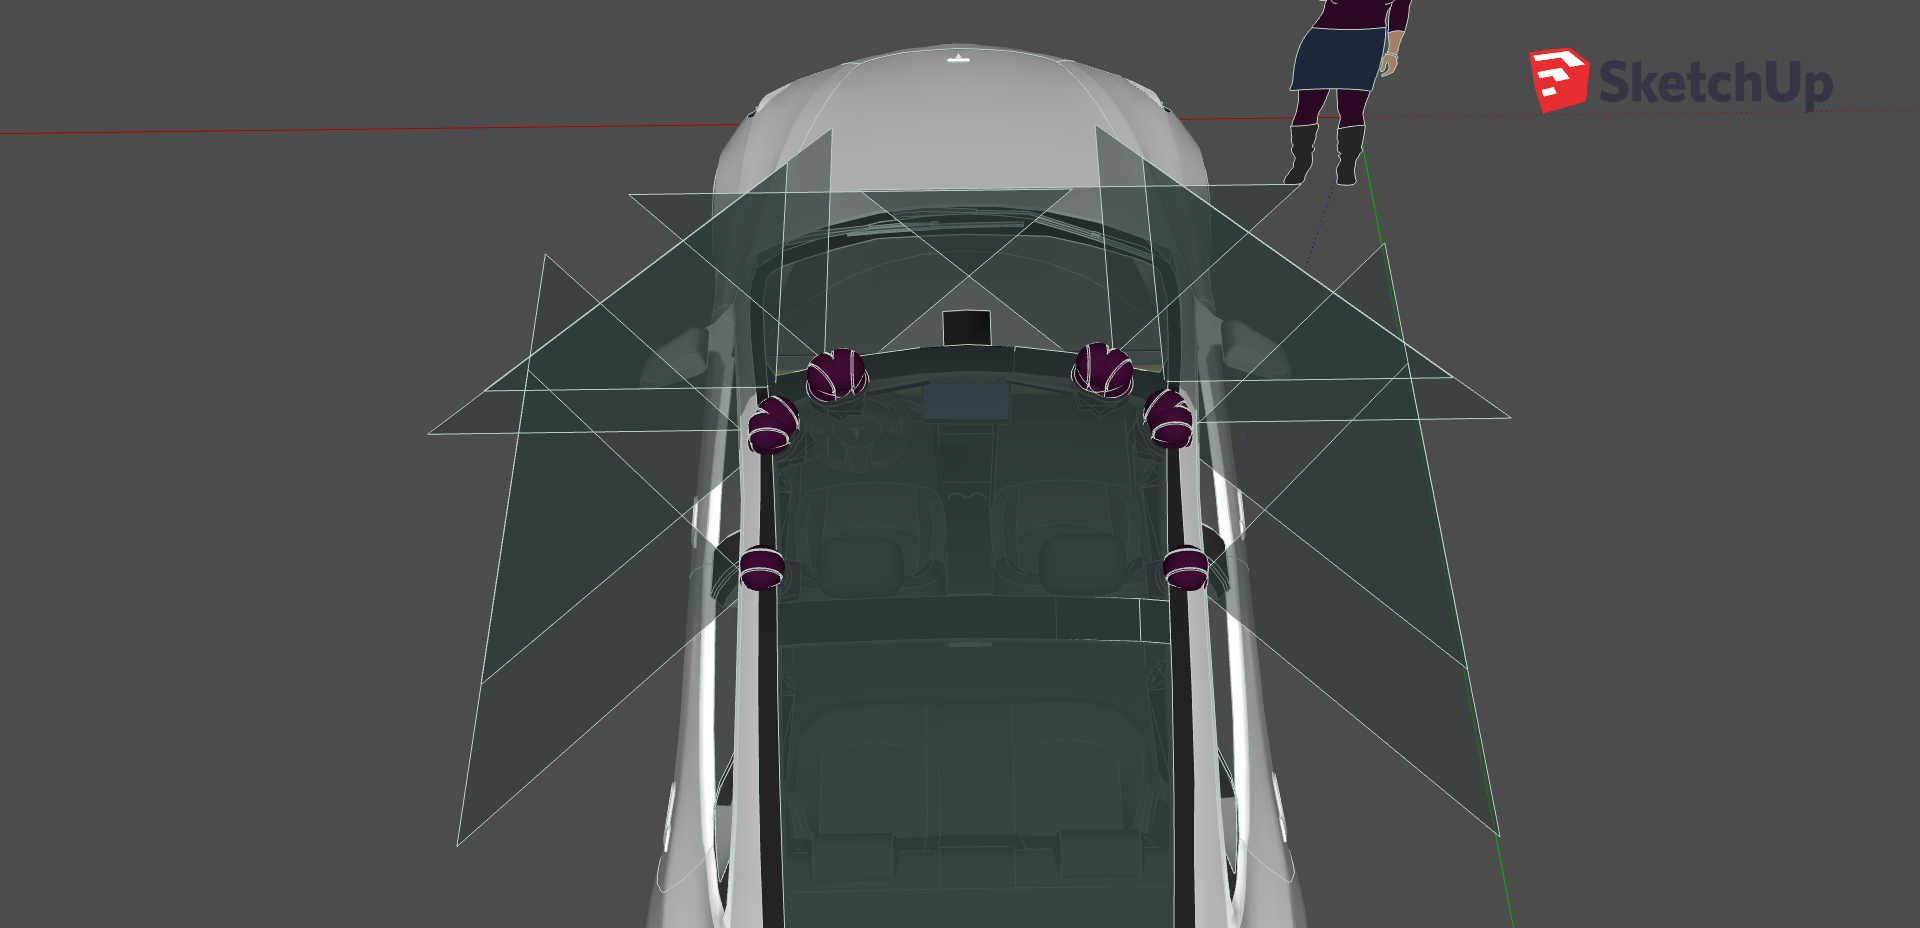
\includegraphics[width=150mm, keepaspectratio]{figures/3dmodel3.png}
    \caption{The stereo camera setting I used on top of the virtual Tesla Model 3}
    \label{fig:3dmodel3}
\end{figure}

In details: 
\begin{itemize}
    \item Front stereo: two cameras looking straight to the front 0.8 meters
          apart
    \item Right corner and left corner stereo cameras: the cameras are on the
          diagonal corners of a 20 cm wide 20cm tall triangle creating two 45\degree
          angled stero vision.
    \item Right and left side stereos are turned 90\degree to the sides and they are apart 0.5 meter.
\end{itemize}
The cameras are 1.5 meters above the ground and they are mounted relative to the
bottom center-point of the vehicle.

The advantage of puting stereo cameras apart to a relatively large distance is
that it increases the accuracy of the stereo block matching algorithm to a
further distances. The drawback however is that a smaller portion of the right
and left side images are going to intersect hence creating a smaller field of
view. However due to the corner stereo cameras this is not a problem for us.

\section{Configuring the simulation}

Carla simulator can be ran in two time-step settings: variable and synchronous.
In real-world perception it is a complex task by itself to synchronize multiple
cameras with each other so that when the algorithm calculates information based
on data from multiple sensors they all correspond to the same moment in time
with an error boundary. In a simulation however we can have the freedom to
synchronize the simulation timesteps themselves and collect all imaging data
between each timestep. Setting Carla to synchronous timestep ensures that all
images in a certain frame are collected and respond to the same moment. 

I used 30FPS timestep setting so that physics calculations are still realistic
but the performance is not too bad. We also have to account for the size of the
generated images: it was good to half the size of the image datasets from a
60FPS setting. Increasing the traffic participants also degrades the
performance. I usually used 200 vehicles and 100 pedestrians for each map, that
resulted in realistic traffic scenarios. 

I recorded different scenarios of approximately 1 minute, which means 1800
frames on 30FPS. On the Titan X machine it it took 15 minutes to render 1
simulation minute, i.e. it ran the simulation with 2FPS. Note, this is different
from the simulation time-step which we fixed to 30FPS.  Since I collect 10 images
in each frame it results in a dataset of 18000 images.

The camera setting I used is an undistorted camera that takes $1280\times720$
resolution images, i.e. HD 720p images, compressed with JPEG to yield a
reasonable size. This way one image is on average 215 kilobytes instead of 1MB
which is a good compression rate and this was the limit where I did not see
any difference in detection accuracy.

In a real-world systems images go straight to the GPU and CPU unit and they get
downscaled to the choosen size before feeding into the algorithm. I had to
resort to compression because of the research nature of the project: I reran
and tested the accuracy of the detector many times on the same dataset.

Using an undistorted camera matrix only means that we need to use one less back
transformation matrix in the detection calculations. In real-world the intrinsic
camera matrix is calculated and corrected for cameras that are mounted on cars
and it is part of the calculation.

Besides imaging we have the ground truth log data. During the simulation,
besides rendering images I coded a logger that logs the necessary information of
the state of the simulator for each frame. This information is built up in a
json-like dictionary, and at the end of the simulation it is saved to one file,
that I call the framelist.

\section{Extracted data}

Naming the images in an organized way is important to make it easy to read the
images in a structured way upon detection. Each image starts with the number of
the frame it was taken in. Starting the simulator server Carla increases a
frame counter starting with 1. To know which image corresponds to which camera,
the framenumbers are postfixed with a label. \autoref{fig:labeling} shows the
postfixes for each image.

\begin{figure}[!ht]
    \centering
    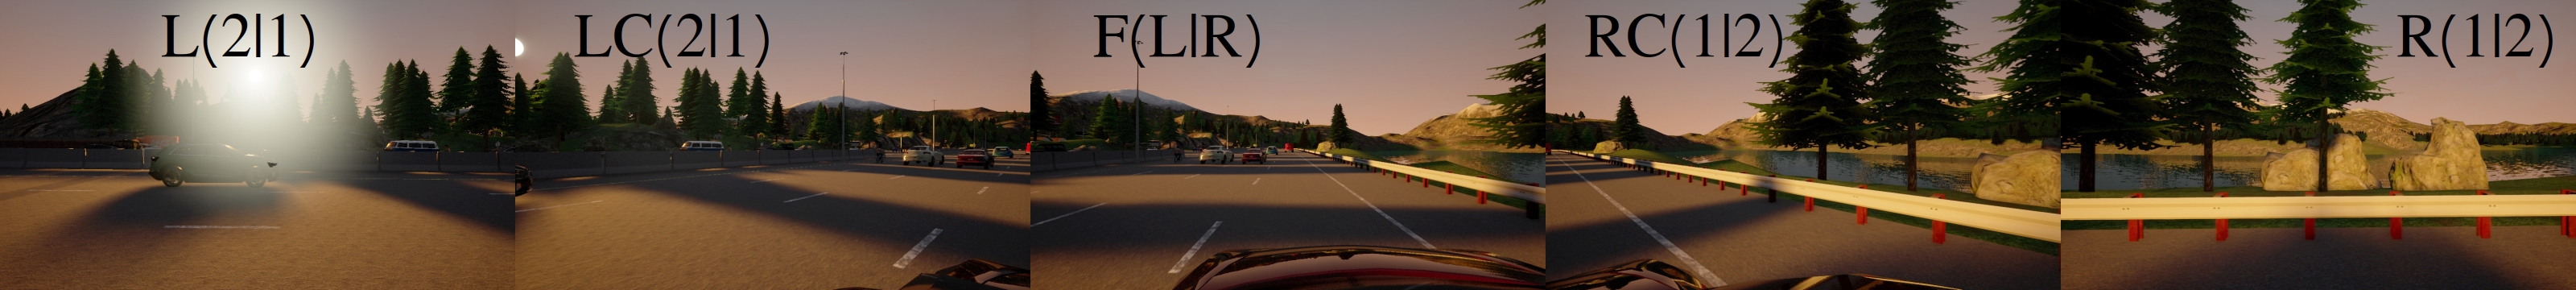
\includegraphics[width=150mm, keepaspectratio]{figures/labeling.jpg}
    \caption{L2/1, R1/2: Right side/Left side first and second cameras, LC(2/1), RC(1/2): Right corner, left corner cameras, FL FR: Front left, front right cameras}
    \label{fig:labeling}
\end{figure}

In each frame I log information about the current state of the simulation. For
the purpouses of the final detector the following information gets logged in each frame:
\begin{itemize}
    \item Frame's number: the value of the frame counter at each frame
    \item For all walker and vehicle actors in a 100 meter radius from the ego car:
          \begin{itemize}
              \item Id: corresponds to the actor's unique id among other actors.
              \item Relative position: X, Y, Z coordinate of the actor in the CARLA
                    coordinate system (see \autoref{fig:carlacoords})
              \item Distance: Euclidean distance from the ego car
          \end{itemize}
    \item Waypoints: these are center and left-right points of the lane the egocar is currently in up
          to 30 points forward. These were meant to be the ground-truth data for
          lane-detection
\end{itemize}

This information is then exported into a JSON file with the following format:
\begin{lstlisting}[language=]
frameList: [
    {
        frame: Number,
        actors: [
            {
                type: car|pedestrian,
                id: Number,
                relative_position: {
                    x: Number,
                    y: Number,
                    z: Number,
                }
            },
        ],
    },
]
\end{lstlisting}

For a one-minute simulation the ground-truth json file is approximately 20
megabytes. It isn't optimal to save information like this for longer
simulations. In those cases it is recommended to use a binary format. Carla
provides a way to save binary information of the recording but unfortunately
there were issues with recording that way, so I ended up with this custom log
format. However it ended up being beneficial, because the webvisualizer
simply loads the json files (detection and ground truth) into two JavaScript
objects.

\section{Detector}

The algorithm plan is the following: for each stereo pair of images calculate
the disparity map with a stereo block matching algorithm. Then detetect objects
and their segmentation mask (instance segmentation) with a state-of-the-art
convnet and then extract the disparity data using the segmentaiton mask. Then
use the extracted disparity data to estimate the depth of the detected object and
then reproject to Carla-world coordinates to match the logfile coordinate
system.

\subsection{Detectron2}
Detectron2's~\cite{wu2019detectron2} Mask R-CNN model provides both object
detection and instance segmentation so I decided to use it. Detectron is built
with PyTorch, Facebook's own GPU-aided ML library.

% There are multiple models provided by D

The algorithm runs the detecton prediction only on the left image of each side,
because later on we will need the segmentation mask of the left image to extract
the depth data from the disparity map generated by the stereo block matching
algorithm. 

Before prediction if our ego car falls into the image it is filled with zeros,
i.e. it is occluded ith black color. It is better to use black since it is all
zeros, and therefore convnet is not going to be sensitive for those parts of the
image.

A visualization of the detection results can be seen on \autoref{fig:detection}

\begin{figure}[!ht]
    \centering
    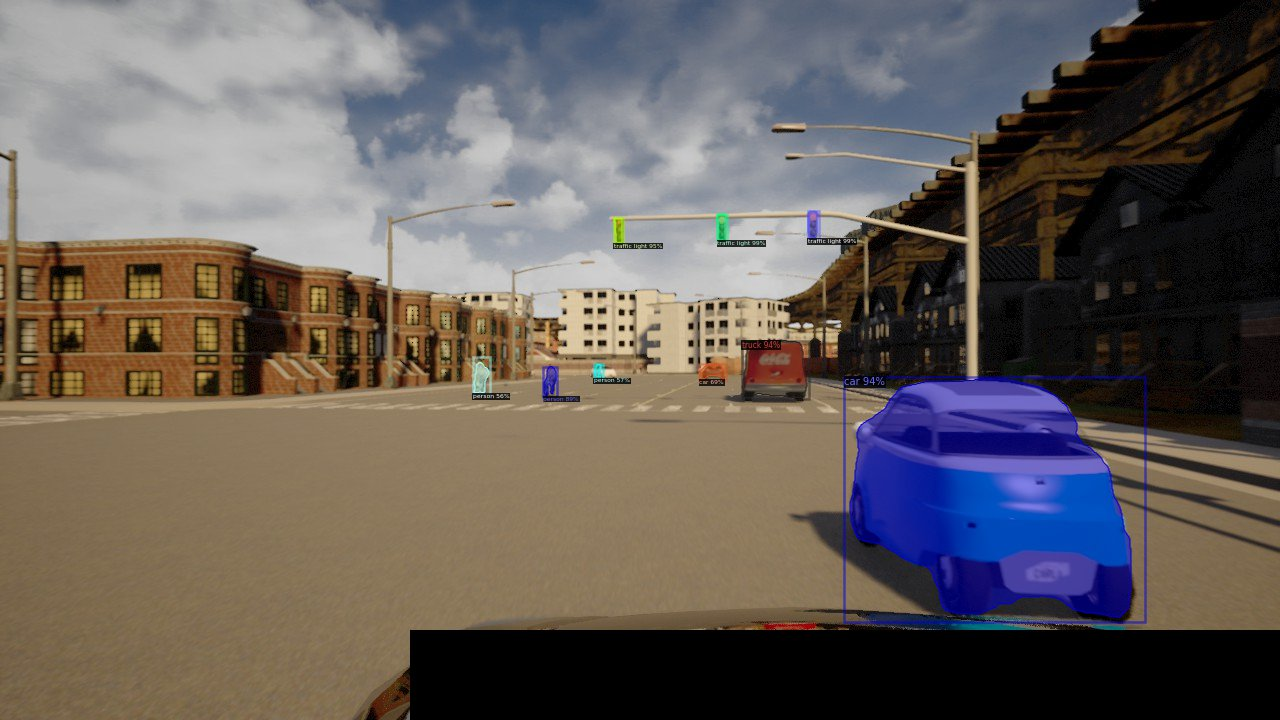
\includegraphics[width=150mm, keepaspectratio]{figures/335DET.jpg}
    \caption{A visualization of the Detectron2 detections and instance segmentation on an ego-occluded image}
    \label{fig:detection}
\end{figure}

\subsection{Depth estimation}
To perform depth estimation I found to easiest way is to use OpenCV a widely
used library in computer vision that includes the stereo processing tools I
needed.
\subsubsection{OpenCV}
OpenCV is a library of programming functions mainly aimed at real-time computer
vision originally developed by Intel. The library is cross-platform and free for
use. It provides traditional Computer Vision tools such as the stereo
correspondence algorithm using block matching~\cite{5489515} and an advanced
version of it the Semi-Global Block Matching method (SGBM)~\cite{4359315} that I used
for the stereo disparity map calculation.
\subsubsection{Stereo Block Matching Algorithm}
The Stereo Block Matching Algorithm works by comparing the neighborhood of a
pixel to each neighborhood of the row of the other image - the measure of
similarity can be different, but usually the mean squared error is used. Usually
before using the stereo block matchin algorithm a camera calibration is
required. This happens with the chessboard calibration method
\footnote{Chessboard calibration in OpenCV \url{https://docs.opencv.org/master/dc/dbb/tutorial_py_calibration.html}}
 where a flat checkerboard is displayed in front of the two stereo cameras. The
 calibration algorithm then calculates the distortion for each camera and
 rotation difference between the two cameras to calculate the intrinsic matrix.

 In our case since we record images in a super ideal way: no distortion and
 perfectly parallel cameras we don't need any calibration and application of
 inverse intrinsic matrix before using the SGBM algorithm.

\begin{figure}[!ht]
    \centering
    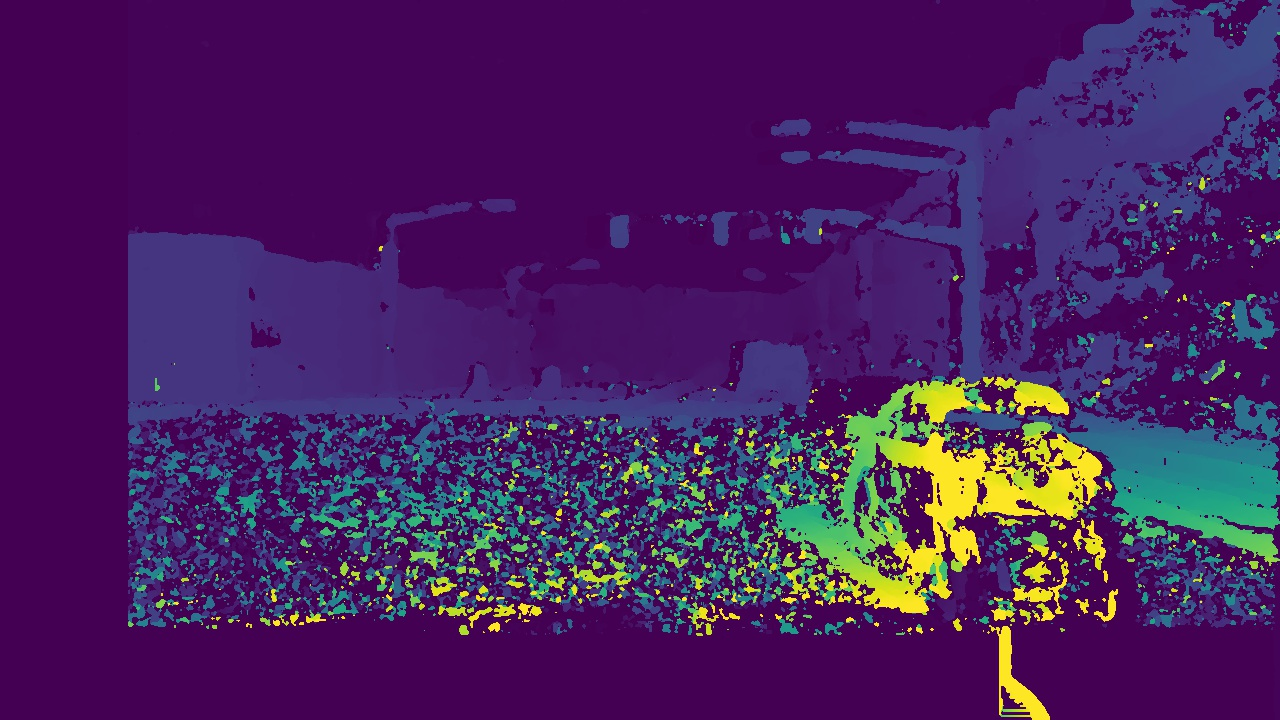
\includegraphics[width=150mm, keepaspectratio]{figures/335DP.jpg}
    \caption{A visualized disparity map result after using OpenCV's StereoSGBM algorithm on the front stereo side}
    \label{fig:disparitymap}
\end{figure}

The StereoBM algorithm considers the left image as the primary, so it will
return a disparitymap that corresponds to the pixels of the left image.

\subsubsection{Triangulation}

Triangulation is a simple method of deriving the depth coordinate when we have
two parallel cameras. \autoref{fig:triangulation} shows the camera setting of
an ideal stereo setting. Recall that each stereo side in our setting is like
this.

\begin{figure}[!ht]
    \centering
    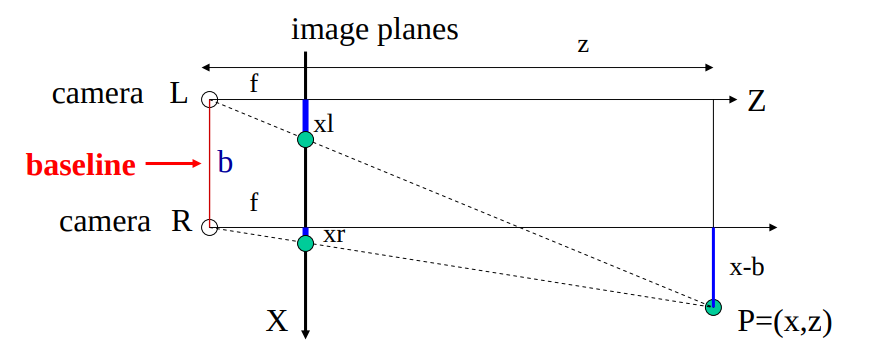
\includegraphics[width=150mm, keepaspectratio]{figures/triangulation.png}
    \caption{An ideal parallel stereo camera model.}
    \label{fig:triangulation}
\end{figure}

If there is a point P in the real world in the field of view of the stereo
camerase, the point will be projected onto different points of both camera's
image plane. If the cameras are set in an ideal parallel stereoscopic setting
then we can easily calculate the depth of the point. The pixel difference
between between pixels correspoonding to the same block can be calculated with
xr-xl. The OpenCV Stereo BM algorithm provides this value for each matched
pixel. From now on all we have to do is use triangulation to calculate the depth
of each pixel. The f corresponds to the focus length and Z corresponds to the
real depth of the point.

The following equations hold true for the figure above from similar triangles.
\begin{align}
    \begin{split}
        \frac{z}{f} = \frac{x}{xl} =  \frac{x-b}{xr} \\
        \frac{z}{f} = \frac{y}{yl} =  \frac{y-b}{yr}
    \end{split}
\end{align}

From this the triangulation is as follows:

\begin{align}
    \begin{split}
        \text{Depth}\;\; Z = \frac{f \cdot b}{xl - xr} =  \frac{f \cdot b}{disparity} \\
        X = \frac{xl \cdot z}{f} \\
        Y = \frac{yl \cdot z}{f}
    \end{split}
\end{align}


\subsubsection{Depth calculation}
Now we know the way to calculate the depth knowing the disparity. The result of
the SGBM, seen on \autoref{fig:disparitymap}, is a 2D array containg valid and
invalid data values. In order to determine the right disparity value
for a detection it is not enough to simple take the values under the mask. The
disparities under a mask contain values for the same object's closest point and
farthest point from the camera. Taking into account the simplifications we
established in the previous chapter there are two solutions to find the distance
of the object: 1.) take the average of the valid disparities under a mask 2.)
take the mode of the disparities. By intuition we would choose taking the
average, however that is going to result in high error and high variance. The
reason is, that the segmentation itself is going to mask values that might not
correspond to the object's disparities. Even a few values that are far from the
average the object's disparities can change the average of the masked
disparities drastically. Using the mode the algorithm yielded much more stable
results, that way it simply is ignores the small inaccuracies of the masking and
disparity error and takes the most dominant disparity value. The visualization
of masking can be seen on \autoref{fig:merged}.

\begin{figure}[!ht]
    \centering
    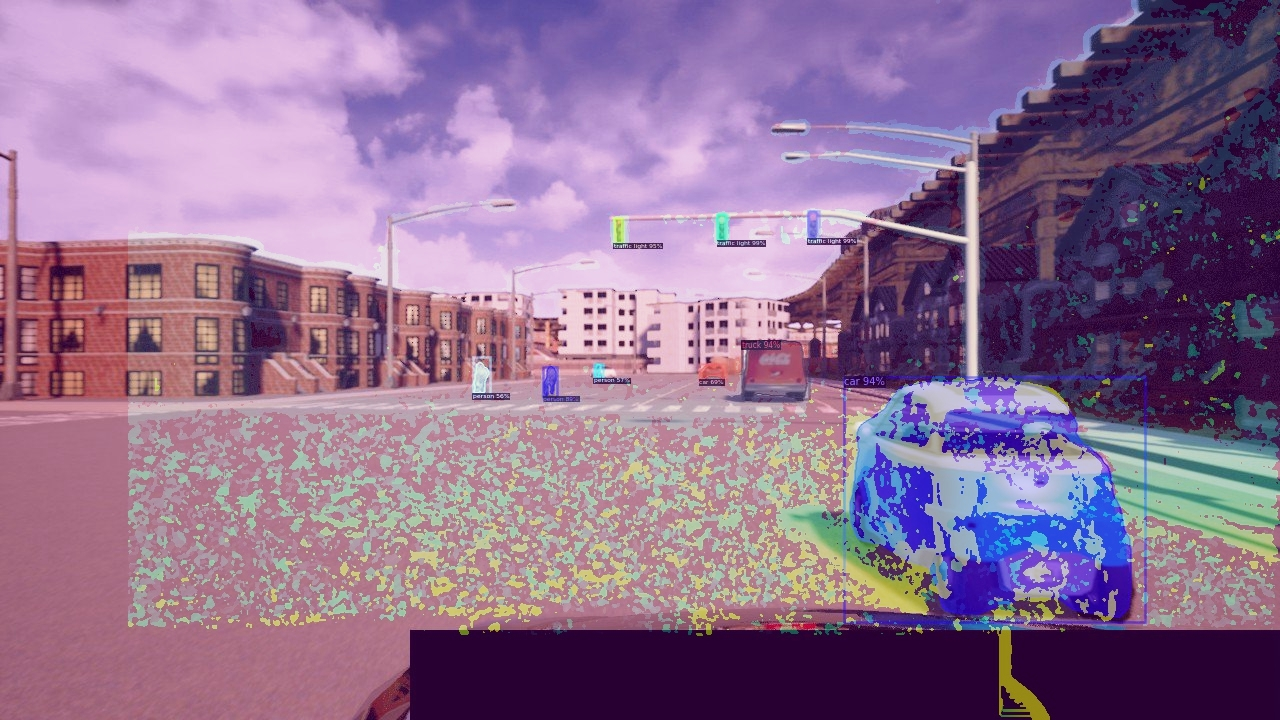
\includegraphics[width=150mm, keepaspectratio]{figures/335merged.jpg}
    \caption{Masking the instance segmentation with the disparitymap filters the necessary values for estimating the vehcile's depth}
    \label{fig:merged}
\end{figure}

\subsection{Back projection}
Each stereo side has a transformation matrix initialized before running the
algorithm. Each matrix is an affine 4x4 transformation matrix, that does the
following in this order: 
\begin{enumerate}
    \item It swapes the axes from the image coordinate system to Carla's coordinate system z->x, x->y, y->z
    \item It rotates the points with the same rotation as the camera
    \item It translates the camera with the same translation for the camerase relative to the vehcile's bottom center point.
  \end{enumerate}

The resulting x, y, z coordinates are the final detection coordinates that get into the detection log.

\subsection{Final pseudo-code}
The final algorithm pseudo-code:
\begin{lstlisting}[language=]
for each frame:
    for each stereo side:
        1. read left and right image
        2. occlude ego from image
        3. compute disparity map using stereo bm.
        4. predict detections and instance segmentation
        for each detection:
            mask disparity map with detection segmentation
            calculate mode of the masked disparity
            apply triangulation and inverse projection
            add actor to frame
    add frame to framelist
save detection list
\end{lstlisting}

\section{Web visualizer}
As I mentioned before in order to compare the detection result and the ground
truth log of each rendering scenario it would be useful to have a visusalization
of the detection replayed. This is similar to the information shown on a monitor
of a self-driving car.

Since I already had experience in Javascript and in ReactJs \footnote{ReactJs
    \url{https://reactjs.org/}} - an easy-to-use web application framework
developed by Facebook - I decided to look for options in 3D visualization. I
found WebViz\footnote{WorldView WebViz \url{https://webviz.io/worldview/}}, a
React library specifically made for 3D visualization of traffic scenarios. It
has a compelling declarative API.

There are two main views in the end product webvisualizer: The video montage and
the 3D visualization (\autoref{fig:webviz2})

The main feature of the webvisualizer is to replay each simulation and see the
original, detection and depthmap videos in synchronization with the 3D
visualizer that displays both the detection log and the ground truth log for
each frame. The webapp is equipped with control buttons that help the control of
the playback. 

\begin{figure}[!ht]
    \centering
    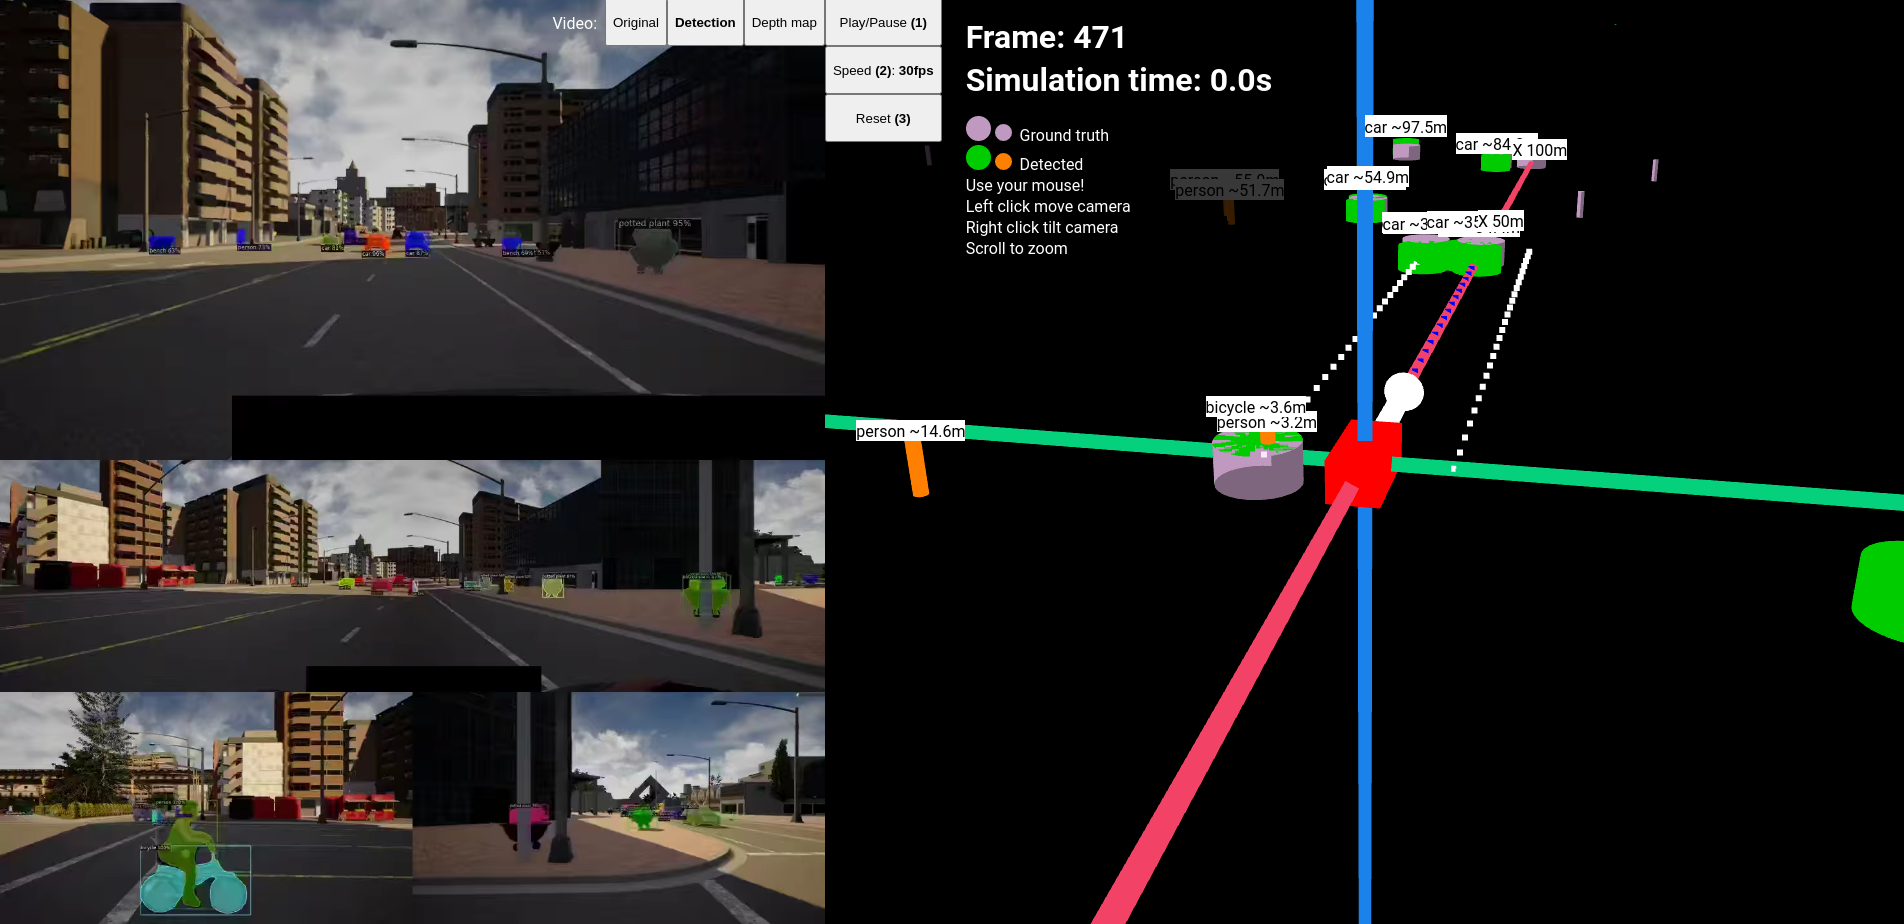
\includegraphics[width=150mm, keepaspectratio]{figures/webviz3.png}
    \caption{Screenshot of the webvisualizer}
    \label{fig:webviz2}
\end{figure}

\begin{figure}[!ht]
    \centering
    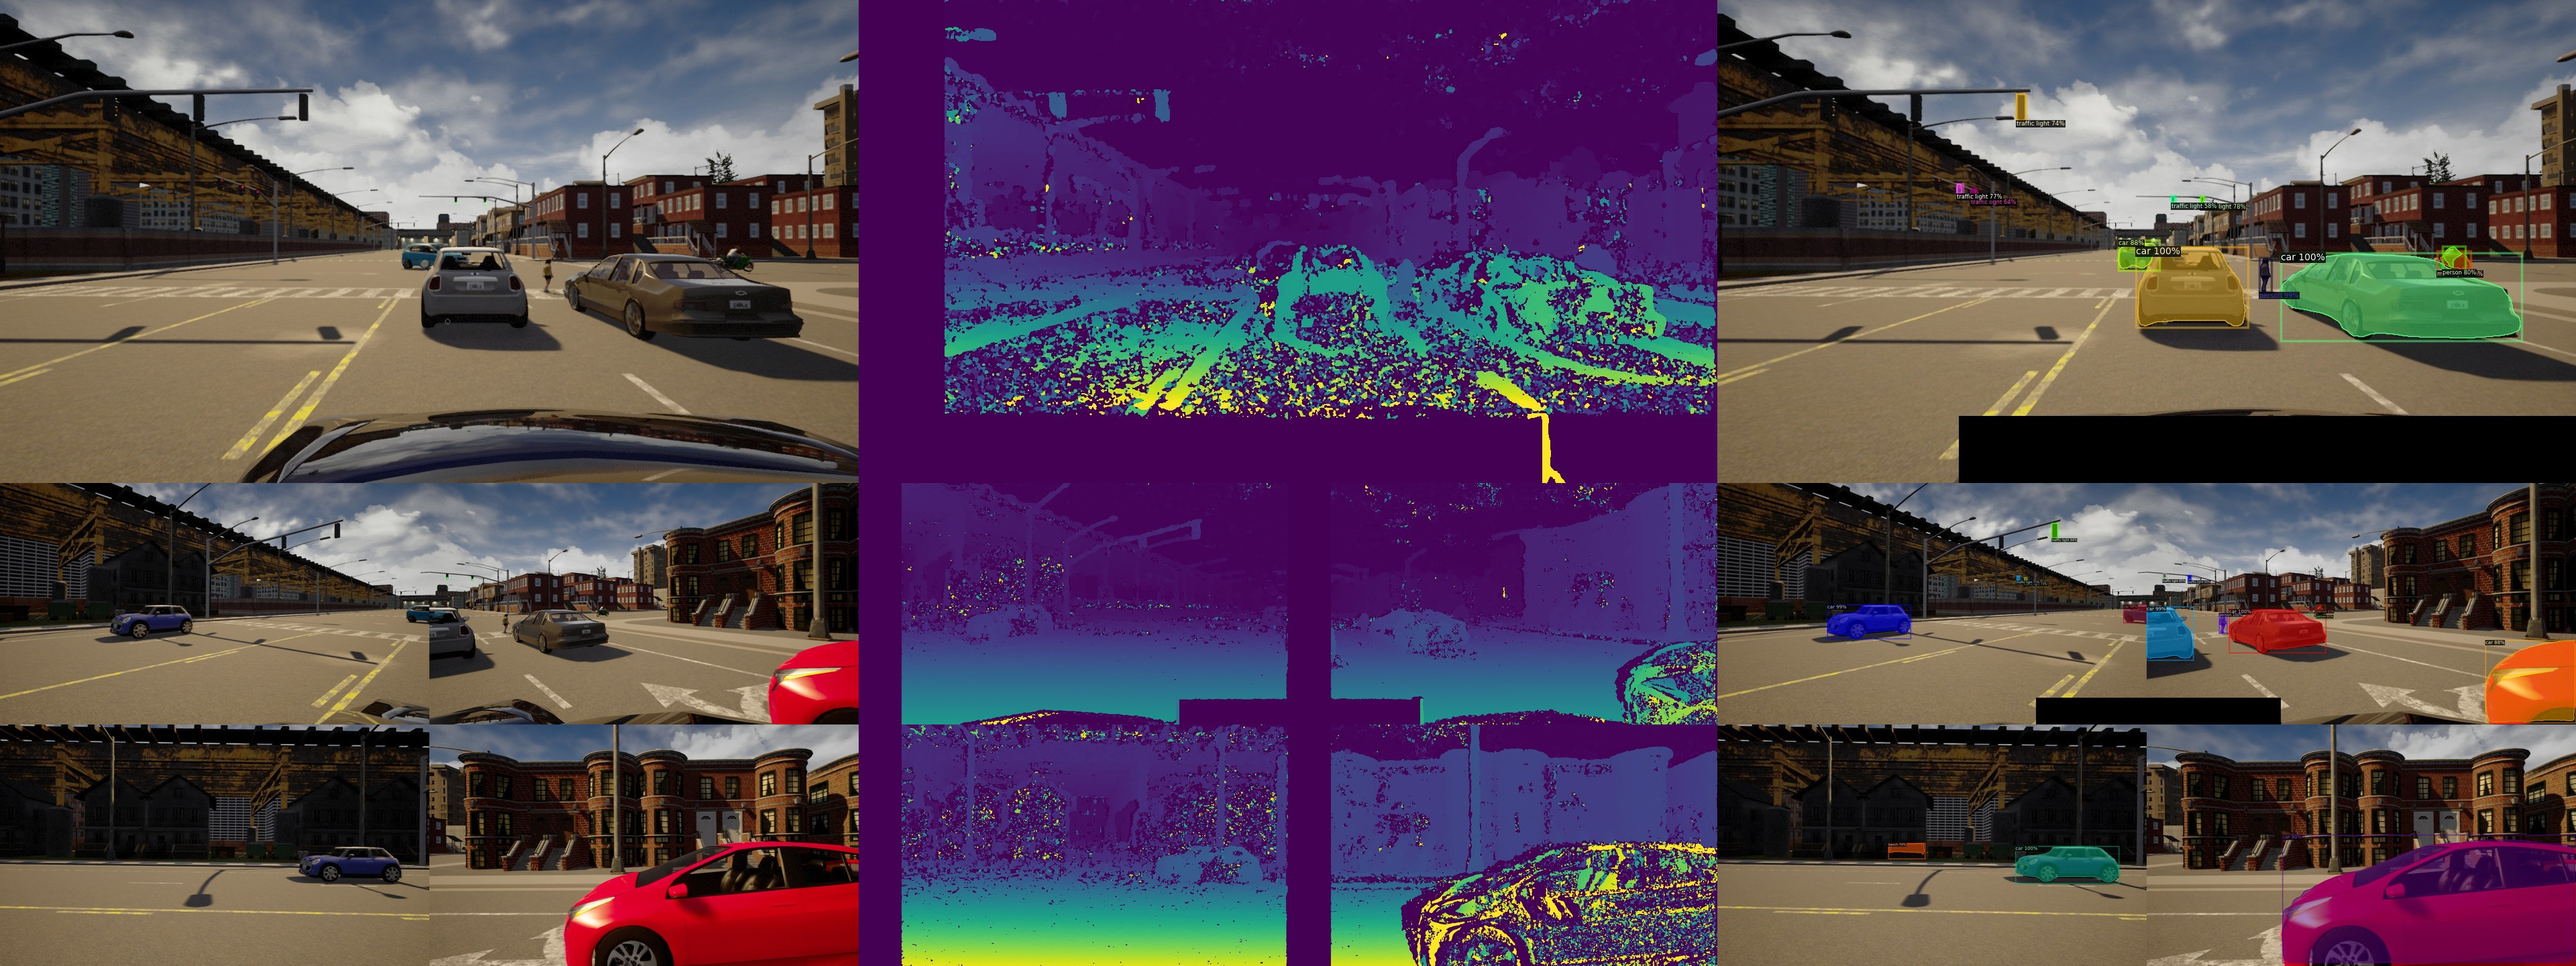
\includegraphics[width=150mm, keepaspectratio]{figures/detmontage.jpg}
    \caption{The montage videos in the webvisalization: original, depthmap, detections}
    \label{fig:detmontage}
\end{figure}


\section{Additonal scripts}

In order to simplify some tasks that included multiple repetitive commands I had
to create some scripts that let me invoke them in one command. One script was to
start the simulator, the ego controller and spawn actors in a choosen map all in
one script. Another useful script was to create a montage of all frames and
immediately create a video and compress it multiple times.

%----------------------------------------------------------------------------
\chapter{Results}
\label{chap:results}
%----------------------------------------------------------------------------

\section{Accuracy}
The best way to see the accuracy of the detector is through the webvisualizer.
The reader is encouraged to visit \url{https://najibghadri.com/msc-thesis/}
where you can interact with with the simulation playback and see each detection.

The reader might notice that most of the time the detected objects are located
closer than the ground truth. Recall, that the depth estimation happens on the
surface of the object. Estimating the centerpoint is difficult. If instead of
working with centerpoints I would have worked with a more complex approach of
first detection orientation or 3D bounding box, ther would be no need for
working with center points. I discuss improvements later on.

\begin{figure}[!ht]
	\centering
	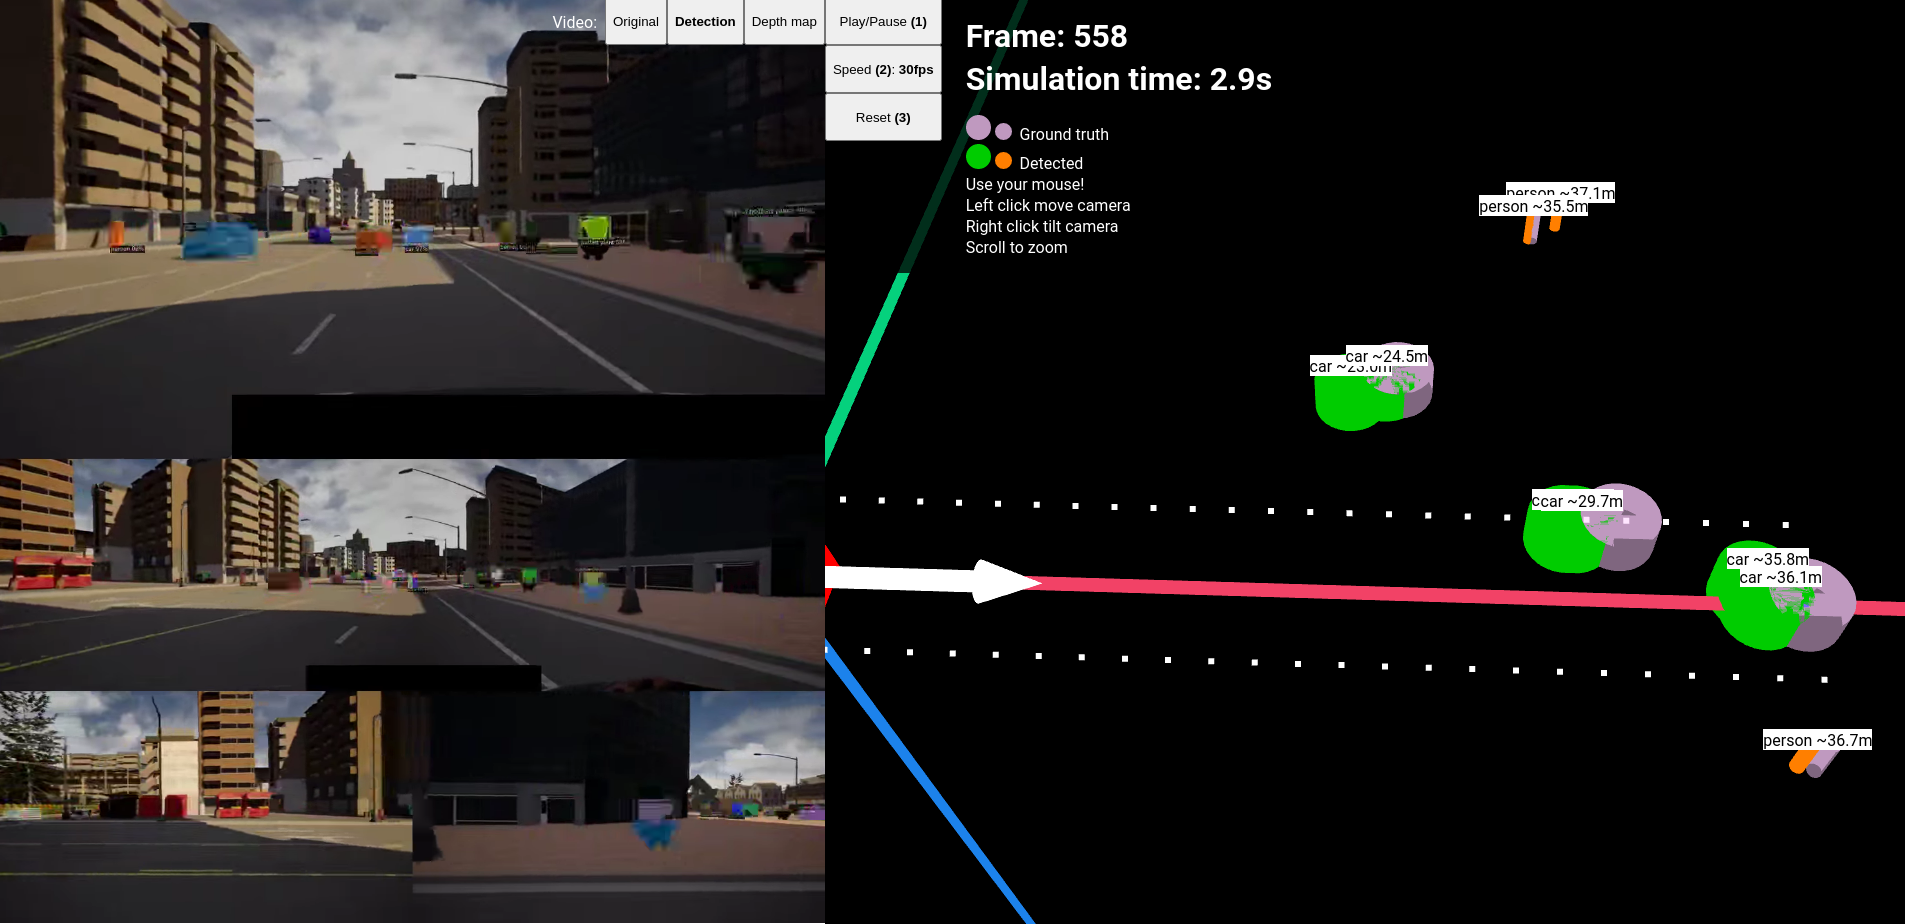
\includegraphics[width=150mm, keepaspectratio]{figures/accuracy.png}
	\caption{General accuraccy of the detector visualized in the webviewer}
	\label{fig:accuracy}
\end{figure}

Genearlly there are no missed objects but there are false positives. Most of the
detections are accurate within ~0.5meters. 

\begin{figure}[!ht]
	\centering
	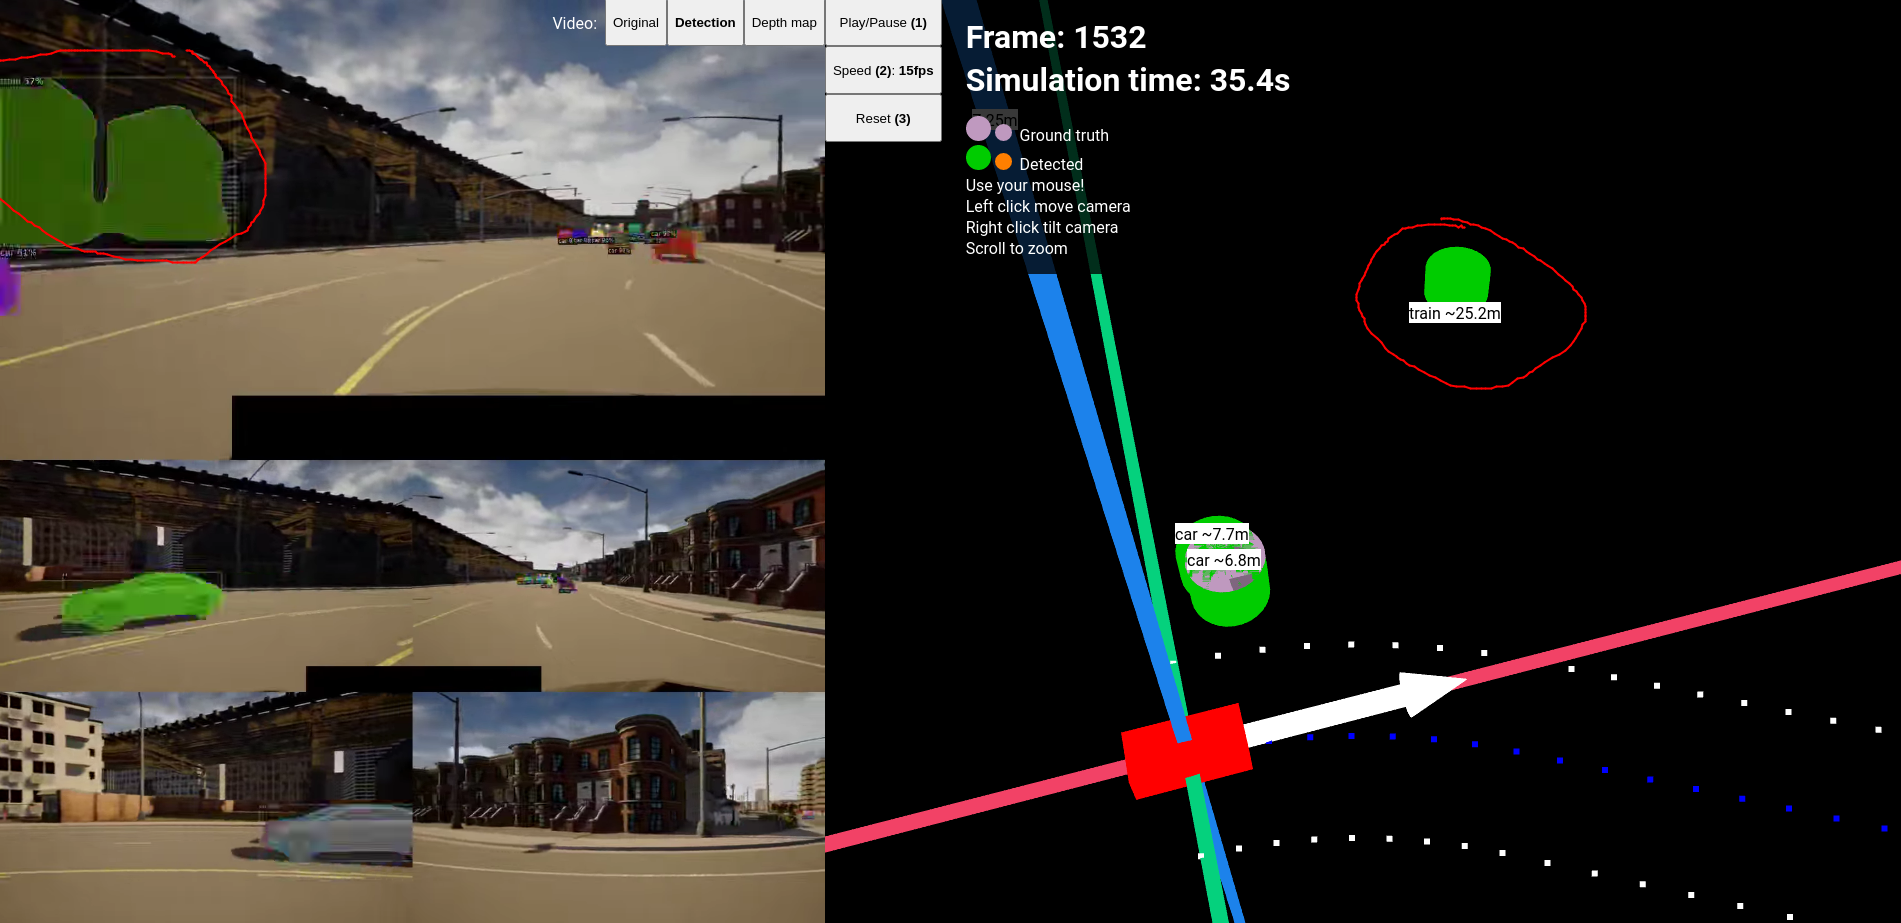
\includegraphics[width=150mm, keepaspectratio]{figures/accfalsepositive.png}
	\caption{False positive detection where a building is detected as a train}
	\label{fig:accfalsepositive}
\end{figure}


Depth estimation is not accurate enough due to the inaccuracy of the
blockmatching algorithm. This can be fixed with the use of LiDar or radio
sensors instead of stereo imaging. Optimal sensor suite is discussed in
Improvements \autoref{chap:improvement}.

Since the setero sides overlap and they see different sides of the detect
objects in the detection log the objects appear as many times as many sides it
appears on as seen on \autoref{fig:accmultidet}. This can be fixed by using tracking and using a shared feature
dictionary. Another solution is to abandon stereo camera based depth estimation
and use mono cameras with radio or lidar sensors for depth estimation with
cameras having a small overlapping region. This would be similar to Tesla's
approach.

\begin{figure}[!ht]
	\centering
	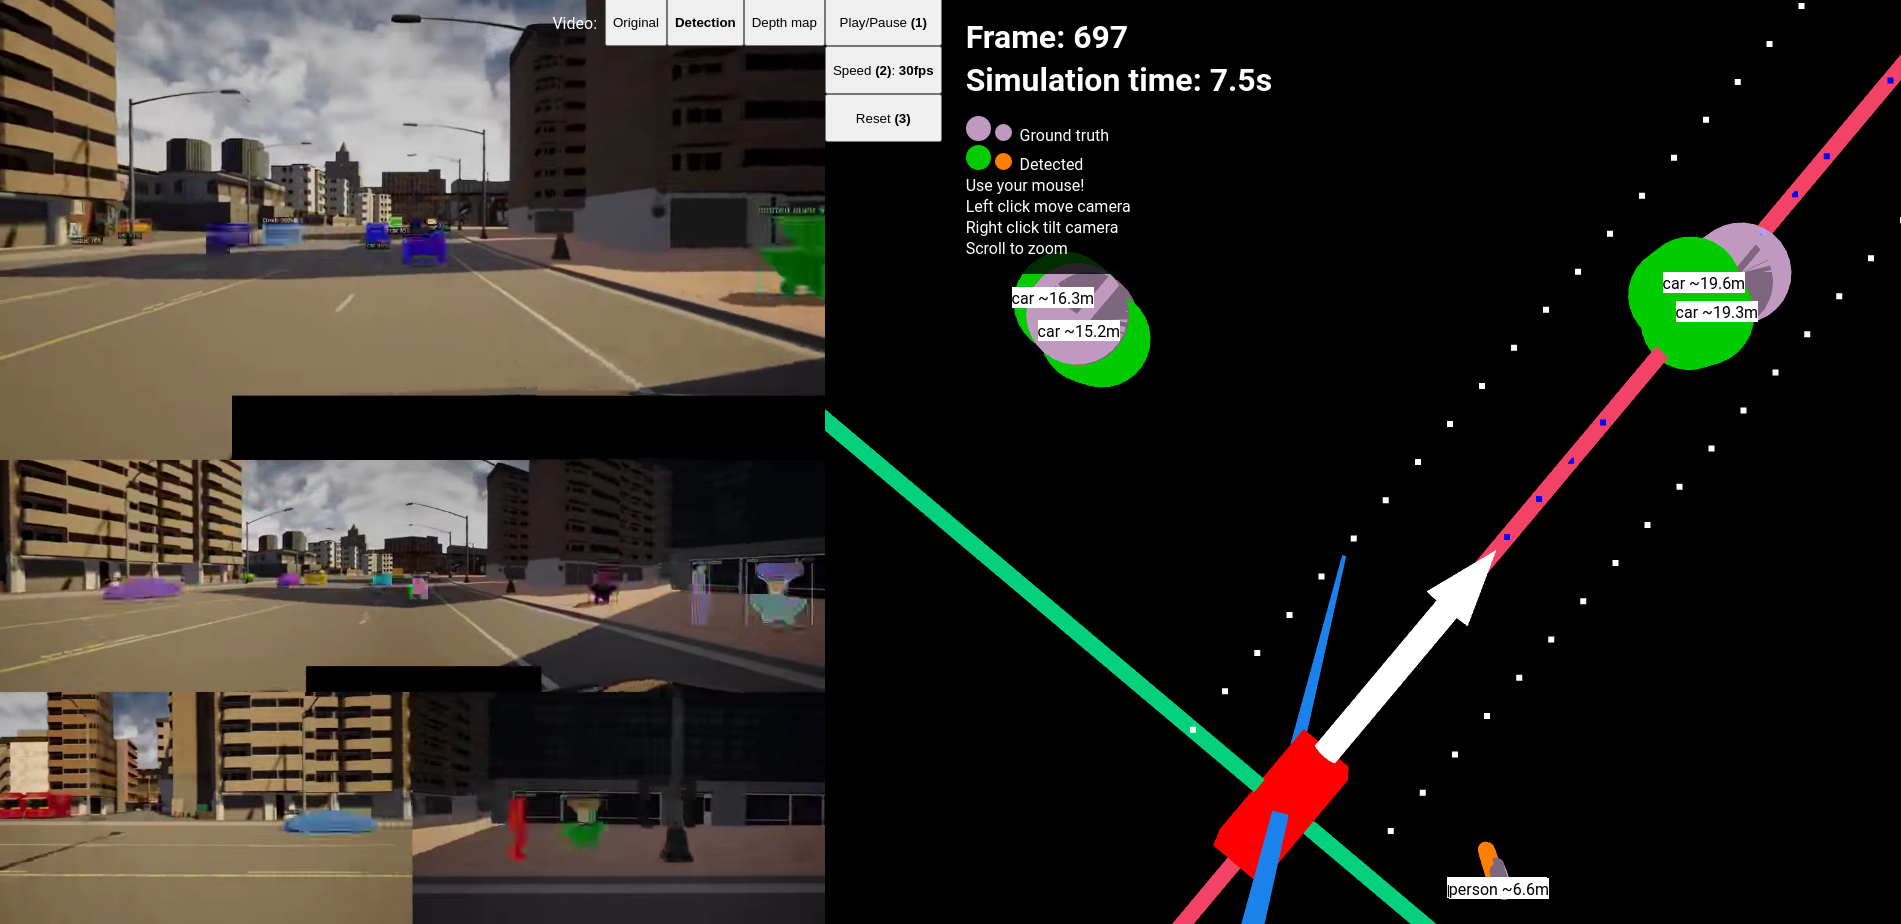
\includegraphics[width=150mm, keepaspectratio]{figures/accmultidet.png}
	\caption{Multiple detections of the same object due to overlapping stereo sides}
	\label{fig:accmultidet}
\end{figure}

Despite these depth estimation can be accurate to 70 meters even as seen on \autoref{fig:accfar}.
\begin{figure}[!ht]
	\centering
	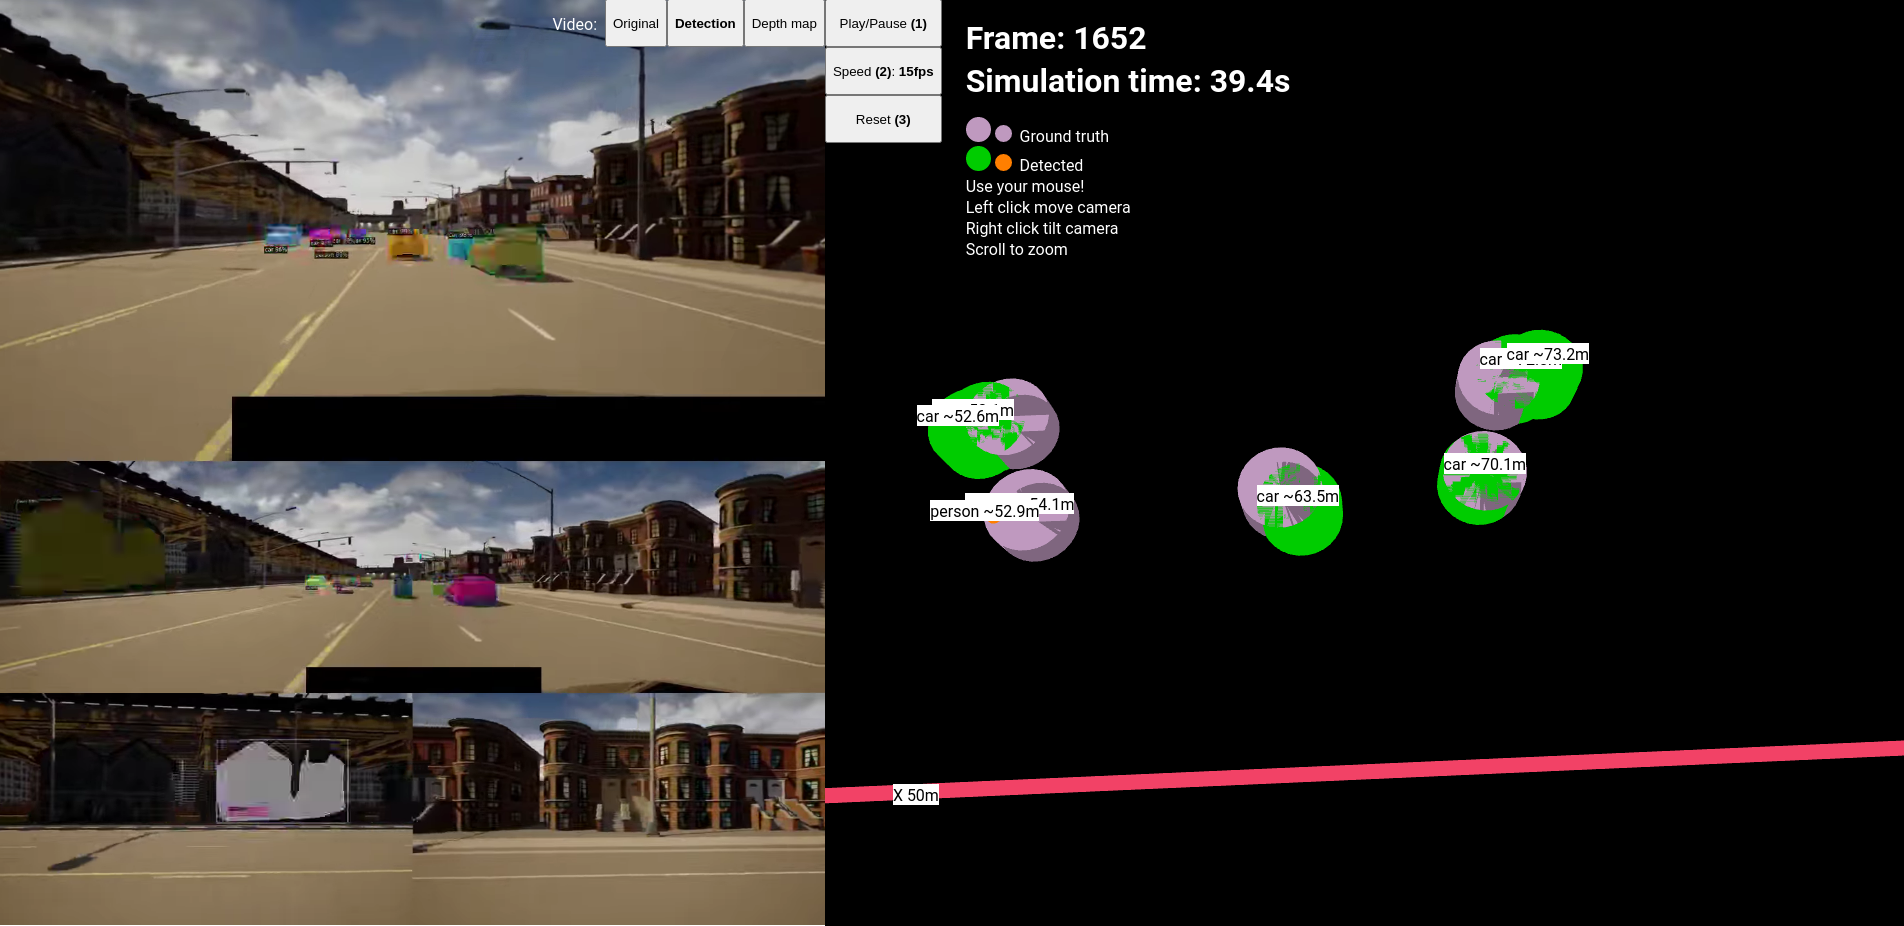
\includegraphics[width=150mm, keepaspectratio]{figures/accfar.png}
	\caption{Relatively accurate depth estimation for far distances of \textasciitilde70 meters}
	\label{fig:accfar}
\end{figure}

An automatic quantification method for the error will be discussed in \autoref{chap:improvement}.

\subsection{Fine tuning}
Choosing different convnet models for Detectron2 can change the performance and
accuracy of the detector. I used the ResNet-101
model~\cite{DBLP:journals/corr/HeZRS15}. ResNet50 is faster but I experienced
more detection misses.

\begin{table}[ht]
	\footnotesize
	\centering
	\begin{tabular}{ l c c }
		\toprule
		Sides       & FPS average \\
		\midrule
		All 5 sides & 0.53 FPS    \\
		One side    & 2.73 FPS    \\
		\bottomrule
	\end{tabular}
	\label{tab:TabularExample}
\end{table}

In \autoref{chap:improvement} imporvements on instance segmentation research
will be discussed that might lead to an improved detection speed over
Detectron2.

\section{Free Z coordinate}
As discussed earlier in \autoref{chap:assumptions} about assumptions, the Z
coordinate (in Carla UE coordinates \autoref{fig:carlacoords}) is disgregarded
in the webvisualization. The accuracy of the Z coordinate is not worse or better
the X and Y coordinates but 

- Car tilt problem - Carla
position problem - Z coordinate hack explain why its ok, CARLA issue Show the
difference!

\section{Dark results}


\section{Hardware requirements}
It wasn't possible for me to evalute the real-timeness of the system simply
because the architecture doesn't allow that. As discussed earlier in
\autoref{chap:carlasim} Nvidia Drive Consteallation has support for HIL
simulation that could be used to test the real-timeness of systems.
%----------------------------------------------------------------------------
\chapter{Experimental results}
%----------------------------------------------------------------------------

A bevezető tartalmazza a diplomaterv-kiírás elemzését, történelmi előzményeit, 
a feladat indokoltságát (a motiváció leírását), az eddigi megoldásokat, 
és ennek tükrében a hallgató megoldásának összefoglalását.

A bevezető szokás szerint a diplomaterv felépítésével záródik, 
azaz annak rövid leírásával, hogy melyik fejezet mivel foglalkozik.

%----------------------------------------------------------------------------
\chapter{Improvement notes}
\label{chap:improvement}
%----------------------------------------------------------------------------
In \autoref{chap:assumptions} I established some simplifications to the system.
In order to create a fully capable scene understanding algorithm the following
improvements are needed.

\section{Tracking and correlation}
In order to measure the accuracy of detections (false positives, false
negatives), it is important to correlate the positive detections with the most
likely ground truth actor. This could be done by finding the closest truth actor
to each detection. This should suffice, because in case there are huge errors,
intead the algorithm should be redesigned fundamentally!

\section{Faster instance segmentation with Yolact++}
A new research has emerged relating instance segmentation,
YOLACT~\cite{yolact-iccv2019} and YOLACT++~\cite{yolact-plus-arxiv2019}\footnote{
Yolact++ repository \url{https://github.com/dbolya/yolact}}, that achieves
30+fps on Titan X for instance segmentation and detection. It is based on YOLO
and uses the same resnet50 model that Detectron2 uses. If this convnet achieves
the same accuracy with a higher fps than it is replaceable with Detectron2.

\section{Optimal sensor suite}
We have seen that companies use many sensors combined not only rgb cameras. In
an optimal setting I would use only one stereo camera setting to the front and
rely on radar and ultrasonic sensors for depth data. Monodepth is also an option
to estimate or correct depth however research is still ongoing and it might not
be a stable method.

\section{Keypoint based detection and orientation}
Orientation, keypoint detection, wheel, etc detection
Depth not based on center point

\section{Data correction}


The percieved information must be corrected with the car's gyroscopic data,
because cameras get tilted Car position, tilt, velocity detection and correction,
odometric correction


\section{Depth correction}
Size based depth correction
Parallax motion based depth correction
\subsection{Size based}
\subsection{Monodepth}
\subsection{Parallax motion}
\section{Lane, path and road detection}
Road segmentation, path  based on other actors
Drivable area reconstruction from other actors - more robust


\section{3D reconstruction}
Voxel reconstruction of actors
\section{Traffic light understanding}
\section{Foreign object detection}
White list based - difficult problem! (https://link.springer.com/article/10.1186/s13640-018-0261-2)

\section{Unsupervised learning methods}
One of the most exciting improvement after all improvements above have been
achieved is to research and implement Energy based models for self-driving cars,
I recommend reading the paper "A tutorial on energy-based
learning"~\cite{Lecun98gradient-basedlearning} by Yann LeCun et al.
%----------------------------------------------------------------------------
\chapter{Conclusion}
\label{chap:conclusion}
%----------------------------------------------------------------------------

Working on this thesis has been a unique experience because the whole filed
was new to me before getting into it. Usually thesis projects require that the
student works on the same project for 4 semesters, however I took a different
road unfortunately or not. I did my previous research work in Web APplications
and Applied blockchain technology. Then I took an optional a deep learning class
and it sparked my interest for AI even more. Taking this project was a risk and
I had to learn about basic computer vision processing methods, algorithms, 3D
vision, the camera model, convolutional neural networks and deep learning and
even a little bit of game engines because of the simulator. But in the end I
learned a lot of things and I hope I can use this knowledge soon in a nice AI
company perhaps one that works on autopilots.

The final scene understanding algorithm is not a system that can be applied by
itself in a real scenaro, however it builds on the same basic ideas for scene
understanding for cars. The work of companies like Tesla and Waymo constitues
many top researchers in the field. In Hungary this market is yet in early
stages but companies like BOSCH or a smaller company like AIMotive are already
present and working on the field with a good pace.


% Acknowledgements
%~~~~~~~~~~~~~~~~~~~~~~~~~~~~~~~~~~~~~~~~~~~~~~~~~~~~~~~~~~~~~~~~~~~~~~~~~~~~~~~~~~~~~~
%----------------------------------------------------------------------------
\chapter*{\koszonetnyilvanitas}\addcontentsline{toc}{chapter}{\koszonetnyilvanitas}
%----------------------------------------------------------------------------

I would like to thank my supervisor, PhD student, Márton Szemenyei for the help,
trust, and the many advices I got during creating this project. I would also like
to thank my previous supervisor Dr. Balázs Goldschmidt for his support in work I
had done before starting this project. I would also like to thank my closest
friends, and most importantly my family for the all-time support.

%%%%
% %----------------------------------------------------------------------------
\chapter{\LaTeX-eszközök}
\label{sec:LatexTools}
%----------------------------------------------------------------------------
\section{A szerkesztéshez használatos eszközök}
%----------------------------------------------------------------------------
Ez a sablon TeXstudio 2.8.8 szerkesztővel készült. A TeXstudio egy
platformfüggetlen, Windows, Linux és Mac OS alatt is elérhető
\LaTeX-szerkesztőprogram számtalan hasznos szolgáltatással
(\refstruc{fig:TeXstudio}). A szoftver ingyenesen letölthető\footnote{A
TeXstudio hivatalos oldala: \url{http://texstudio.sourceforge.net/}}.

\begin{figure}[!ht]
\centering
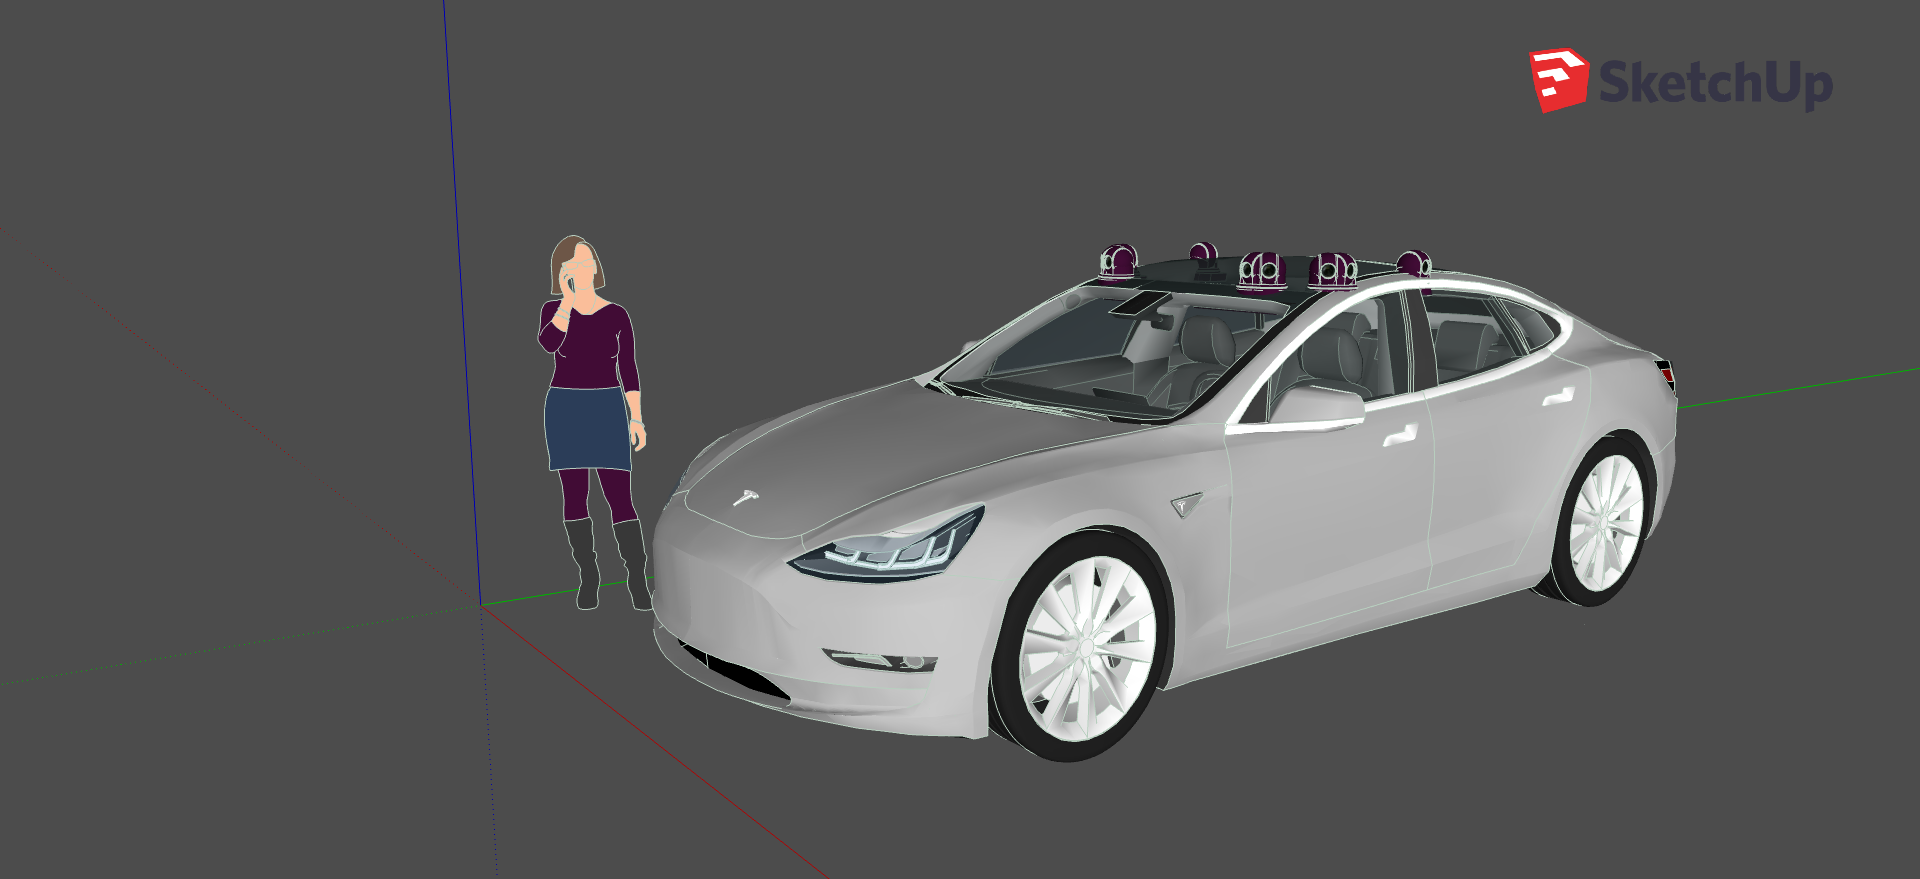
\includegraphics[width=150mm, keepaspectratio]{figures/3dmodel1.png}
\caption{A TeXstudio \LaTeX-szerkesztő.}
\label{fig:TeXstudio}
\end{figure}

A TeXstudio telepítése után érdemes még letölteni a magyar nyelvű
helyesírásellenőrző-szótárakat hozzá. A TeXstudio az OpenOffice-hoz használatos
formátumot tudja kezelni. A TeXstudio beállításainál a \verb+General+ fülön a
\verb+Dictionaries+ résznél tudjuk megadni, hogy melyik szótárat használja.

Egy másik használható Windows alapú szerkesztőprogram a LEd\footnote{A LEd
hivatalos oldala: \url{http://www.latexeditor.org/}} (LaTeX Editor), a TeXstudio
azonban stabilabb, gyorsabb, és jobban használható.

%----------------------------------------------------------------------------
\section{A dokumentum lefordítása Windows alatt}
%----------------------------------------------------------------------------
A TeXstudio és a LEd kizárólag szerkesztőprogram (bár az utóbbiban DVI-nézegető
is van), így a dokumentum fordításához szükséges eszközöket nem tartalmazza.
Windows alatt alapvetően két lehetőség közül érdemes választani: MiKTeX
(\url{http://miktex.org/}) és TeX Live (\url{http://www.tug.org/texlive/})
programcsomag. Az utóbbi működik Mac OS X, GNU/Linux alatt és Unix-származékokon
is. A MiKTeX egy alapcsomag telepítése után mindig letölti a használt
funkciókhoz szükséges, de lokálisan hiányzó \TeX-csomagokat, míg a TeX Live DVD
ISO verzóban férhető hozzá. Ez a dokumentum TeX Live 2008 programcsomag
segítségével fordult, amelynek DVD ISO verziója a megadott oldalról letölthető.
A sablon lefordításához a disztribúcióban szereplő \verb+magyar.ldf+ fájlt a
\verb+http://www.math.bme.hu/latex/+ változatra kell cserélni, vagy az utóbbi
változatot be kell másolni a projekt-könyvtárba (ahogy ezt meg is tettük a
sablonban) különben anomáliák tapasztalhatók a dokumentumban (pl. az ábra- és
táblázat-aláírások formátuma nem a beállított lesz, vagy bizonyos oldalakon
megjelenik alapértelmezésben egy fejléc). A TeX Live 2008-at még nem kell külön
telepíteni a gépre, elegendő DVD-ről (vagy az ISO fájlból közvetlenül, pl.
DaemonTools-szal) használni.

Ha a MiKTeX csomagot használjuk, akkor parancssorból a következő módon tudjuk
újrafordítani a teljes dokumentumot:

\begin{lstlisting}[language=bash,frame=single,float=!ht]
$ texify -p thesis.tex
\end{lstlisting}

A \verb+texify+ parancs a MiKTex programcsomag \verb+miktex/bin+ alkönyvtárában
található. A parancs gondoskodik arról, hogy a szükséges lépéseket (fordítás,
hivatkozások generálása stb.) a megfelelő sorrendben elvégezze. A \verb+-p+
kapcsoló hatására PDF-et generál. A fordítást és az ideiglenes fájlok törlését
elvégezhetjük a sablonhoz mellékelt \verb+manual_build.bat+ szkript segítségével
is.

A \TeX-eszközöket tartalmazó programcsomag binárisainak elérési útját gyakran be
kell állítani a szerkesztőprogramban, például TeXstudio esetén legegyszerűbben
az \verb+Options / Configure TeXstudio... / Commands+ menüponttal előhívott
dialógusablakban tehetjük ezt meg.

A PDF-\LaTeX~használata esetén a generált dokumentum közvetlenül PDF-formátumban
áll rendelkezésre. Amennyiben a PDF-fájl egy PDF-nézőben (pl. Adobe Acrobat
Reader vagy Foxit PDF Reader) meg van nyitva, akkor a fájlleírót a PDF-néző
program tipikusan lefoglalja. Ilyen esetben a dokumentum újrafordítása
hibaüzenettel kilép. Ha bezárjuk és újra megnyitjuk a PDF dokumentumot, akkor
pedig a PDF-nézők többsége az első oldalon nyitja meg a dokumentumot, nem a
legutóbb olvasott oldalon. Ezzel szemben például az egyszerű és ingyenes
\textcolor{blue}{Sumatra PDF} nevű program képes arra, hogy a megnyitott
dokumentum megváltozását detektálja, és frissítse a nézetet az aktuális oldal
megtartásával.

%----------------------------------------------------------------------------
\section{Eszközök Linuxhoz}
%----------------------------------------------------------------------------
Linux operációs rendszer alatt is rengeteg szerkesztőprogram van, pl. a KDE
alapú Kile jól használható. Ez ingyenesen letölthető, vagy éppenséggel az adott
Linux-disztribúció eleve tartalmazza, ahogyan a dokumentum fordításához
szükséges csomagokat is. Az Ubuntu Linux disztribúciók alatt például legtöbbször
a \verb+texlive-*+ csomagok telepítésével használhatók a \LaTeX-eszközök. A
jelen sablon fordításához szükséges csomagok (kb. 0,5 GB) az alábbi paranccsal
telepíthetők:

\begin{lstlisting}[language=bash,morekeywords={sudo,apt\-get},alsoletter={-},breaklines=true]
$ sudo apt-get install texlive-latex-extra texlive-fonts-extra texlive-fonts-recommended texlive-xetex texlive-science
\end{lstlisting}

Amennyiben egy újabb csomag hozzáadása után hiányzó fájlra utaló hibát kapunk a
fordítótól, telepítenünk kell az azt tartalmazó TeX Live csomagot. Ha pl. a
\verb+bibentry+ csomagot szeretnénk használni, futtassuk az alábbi parancsot:

\begin{lstlisting}[language=bash,morekeywords={apt\-cache},alsoletter={-},breaklines=true]
$ apt-cache search bibentry
texlive-luatex - TeX Live: LuaTeX packages
\end{lstlisting}

Majd telepítsük fel a megfelelő TeX Live csomagot, jelen esetben a
`texlive-lualatex`-et. (Egy LaTeX csomag több TeX Live csomagban is
szerepelhet.)

Ha gyakran szerkesztünk más \LaTeX dokumentumokat is, kényelmes és biztos
megoldás a teljes TeX Live disztribúció telepítése, ez azonban kb. 4 GB helyet
igényel.

\begin{lstlisting}[language=bash,morekeywords={sudo,apt\-get},alsoletter={-},breaklines=true]
sudo apt-get install texlive-full
\end{lstlisting}

% %----------------------------------------------------------------------------
\chapter{A dolgozat formai kivitele}
%----------------------------------------------------------------------------
Az itt található információk egy része a BME VIK Hallgatói Képviselet által készített ,,Utolsó félév a villanykaron'' c. munkából lett kis változtatásokkal átemelve. Az eredeti dokumentum az alábbi linken érhető el: \url{http://vik.hk/hirek/diplomafelev-howto-2015}.

%----------------------------------------------------------------------------
\section{A dolgozat kimérete}
%----------------------------------------------------------------------------
Szakdolgozat esetében minimum 30, 45 körüli ajánlott oldalszám lehet az iránymutató. De mindenképp érdemes rákérdezni a konzulensnél is az elvárásokra, mert tanszékenként változóak lehetnek az elvárások.

Mesterképzésen a Diplomatervezés 1 esetében a beszámoló még inkább az Önálló laboratóriumi beszámolókhoz hasonlít, tanszékenként eltérő formai követelményekkel, -- egy legalább 30 oldal körüli dolgozat az elvárt -- és az elmúlt fél éves munkáról szól. De egyben célszerű, ha ez a végleges diplomaterv alapja is. (A végleges 60-90 oldal körülbelül a hasznos részre nézve)


%----------------------------------------------------------------------------
\section{A dolgozat nyelve}
%----------------------------------------------------------------------------
Mivel Magyarországon a hivatalos nyelv a magyar, ezért alapértelmezésben magyarul kell megírni a dolgozatot. Aki külföldi posztgraduális képzésben akar részt venni, nemzetközi szintű tudományos kutatást szeretne végezni, vagy multinacionális cégnél akar elhelyezkedni, annak célszerű angolul megírnia diplomadolgozatát. Mielőtt a hallgató az angol nyelvű verzió mellett dönt, erősen ajánlott mérlegelni, hogy ez mennyi többletmunkát fog a hallgatónak jelenteni fogalmazás és nyelvhelyesség terén, valamint -- nem utolsó sorban -- hogy ez mennyi többletmunkát fog jelenteni a konzulens illetve bíráló számára. Egy nehezen olvasható, netalán érthetetlen szöveg teher minden játékos számára.

%----------------------------------------------------------------------------
\section{A dokumentum nyomdatechnikai kivitele}
%----------------------------------------------------------------------------
A dolgozatot A4-es fehér lapra nyomtatva, 2,5 centiméteres margóval (+1~cm kötésbeni), 11--12 pontos betűmérettel, talpas betűtípussal és másfeles sorközzel célszerű elkészíteni.

Annak érdekében, hogy a dolgozat külsőleg is igényes munka benyomását keltse, érdemes figyelni az alapvető tipográfiai szabályok betartására~\cite{Jeney}.

% % !TeX spellcheck = hu_HU
% !TeX encoding = UTF-8
% !TeX program = xelatex
%----------------------------------------------------------------------------
\chapter{A \LaTeX-sablon használata}
%----------------------------------------------------------------------------

Ebben a fejezetben röviden, implicit módon bemutatjuk a sablon használatának módját, ami azt jelenti, hogy sablon használata ennek a dokumentumnak a forráskódját tanulmányozva válik teljesen világossá. Amennyiben a szoftver-keretrendszer telepítve van, a sablon alkalmazása és a dolgozat szerkesztése \LaTeX-ben a sablon segítségével tapasztalataink szerint jóval hatékonyabb, mint egy WYSWYG (\emph{What You See is What You Get}) típusú szövegszerkesztő esetén (pl. Microsoft Word, OpenOffice).

%----------------------------------------------------------------------------
\section{Címkék és hivatkozások}
%----------------------------------------------------------------------------
A \LaTeX~dokumentumban címkéket (\verb+\label+) rendelhetünk ábrákhoz, táblázatokhoz, fejezetekhez, listákhoz, képletekhez stb. Ezekre a dokumentum bármely részében hivatkozhatunk, a hivatkozások automatikusan feloldásra kerülnek.

A sablonban makrókat definiáltunk a hivatkozások megkönnyítéséhez. Ennek megfelelően minden ábra (\emph{figure}) címkéje \verb+fig:+ kulcsszóval kezdődik, míg minden táblázat (\emph{table}), képlet (\emph{equation}), fejezet (\emph{section}) és lista (\emph{listing}) rendre a \verb+tab:+, \verb+eq:+, \verb+sec:+ és \verb+lst:+ kulcsszóval kezdődik, és a kulcsszavak után tetszőlegesen választott címke használható. Ha ezt a konvenciót betartjuk, akkor az előbbi objektumok számára rendre a \verb+\figref+, \verb+\tabref+, \verb+\eqref+, \verb+\sectref+ és \verb+\listref+ makrókkal hivatkozhatunk. A makrók paramétere a címke, amelyre hivatkozunk (a kulcsszó nélkül). Az összes említett hivatkozástípus, beleértve az \verb+\url+ kulcsszóval bevezetett web-hivatkozásokat is a  \verb+hyperref+\footnote{Segítségével a dokumentumban megjelenő hivatkozások nem csak dinamikussá válnak, de színezhetők is, bővebbet erről a csomag dokumentációjában találunk. Ez egyúttal egy példa lábjegyzet írására.} csomagnak köszönhetően aktívak a legtöbb PDF-nézegetőben, rájuk kattintva a dokumentum megfelelő oldalára ugrik a PDF-néző vagy a megfelelő linket megnyitja az alapértelmezett böngészővel. A \verb+hyperref+ csomag a kimeneti PDF-dokumentumba könyvjelzőket is készít a tartalomjegyzékből. Ez egy szintén aktív tartalomjegyzék, amelynek elemeire kattintva a nézegető behozza a kiválasztott fejezetet.

%----------------------------------------------------------------------------
\section{Ábrák és táblázatok}
%----------------------------------------------------------------------------
Használjunk vektorgrafikus ábrákat, ha van rá módunk. PDFLaTeX használata esetén PDF formátumú ábrákat lehet beilleszteni könnyen, az EPS (PostScript) vektorgrafikus képformátum beillesztését a PDFLaTeX közvetlenül nem támogatja (de lehet konvertálni, lásd később). Ha vektorgrafikus formában nem áll rendelkezésünkre az ábra, akkor a  veszteségmentes PNG, valamint a veszteséges JPEG formátumban érdemes elmenteni.  Figyeljünk arra, hogy ilyenkor a képek felbontása elég nagy legyen ahhoz, hogy nyomtatásban is megfelelő minőséget nyújtson (legalább 300 dpi javasolt). A dokumentumban felhasznált képfájlokat a dokumentum forrása mellett érdemes tartani, archiválni, mivel ezek hiányában a dokumentum nem fordul újra. Ha lehet, a vektorgrafikus képeket vektorgrafikus formátumban is érdemes elmenteni az újrafelhasználhatóság (az átszerkeszthetőség) érdekében.

Kapcsolási rajzok legtöbbször kimásolhatók egy vektorgrafikus programba (pl. CorelDraw) és onnan nagyobb felbontással raszterizálva kimenthatők PNG formátumban. Ugyanakkor kiváló ábrák készíthetők Microsoft Visio vagy hasonló program használatával is: Visio-ból az ábrák közvetlenül PDF-be is menthetők.

Lehetőségeink Matlab ábrák esetén:
\begin{itemize}
	\item Képernyőlopás (\emph{screenshot}) is elfogadható minőségű lehet a dokumentumban, de általában jobb felbontást is el lehet érni más módszerrel.
	\item A Matlab ábrát a \verb+File/Save As+ opcióval lementhetjük PNG formátumban (ugyanaz itt is érvényes, mint korábban, ezért nem javasoljuk).
	\item A Matlab ábrát az \verb+Edit/Copy figure+ opcióval kimásolhatjuk egy vektorgrafikus programba is és onnan nagyobb felbontással raszterizálva kimenthatjük PNG formátumban (nem javasolt).
	\item Javasolt megoldás: az ábrát a \verb+File/Save As+ opcióval EPS \emph{vektorgrafikus} formátumban elmentjük, PDF-be konvertálva beillesztjük a dolgozatba.
\end{itemize}
Az EPS kép az \verb+epstopdf+ programmal\footnote{a korábban említett \LaTeX-disztribúciókban megtalálható} konvertálható PDF formátumba. Célszerű egy batch-fájlt készíteni az összes EPS ábra lefordítására az alábbi módon (ez Windows alatt működik).
\begin{lstlisting}[language=]
@echo off
for %%j in (*.eps) do (
  echo converting file "%%j"
  epstopdf "%%j"
)
echo done .
\end{lstlisting}

Egy ilyen parancsfájlt (\verb+convert.cmd+) elhelyeztük a sablon \verb+figures\eps+ könyvtárába, így a felhasználónak csak annyi a dolga, hogy a \verb+figures\eps+ könyvtárba kimenti az EPS formátumú vektorgrafikus képet, majd lefuttatja a \verb+convert.cmd+ parancsfájlt, ami PDF-be konvertálja az EPS fájlt.

Ezek után a PDF-ábrát ugyanúgy lehet a dokumentumba beilleszteni, mint a PNG-t vagy a JPEG-et. A megoldás előnye, hogy a lefordított dokumentumban is vektorgrafikusan tárolódik az ábra, így a mérete jóval kisebb, mintha raszterizáltuk volna beillesztés előtt. Ez a módszer minden -- az EPS formátumot ismerő -- vektorgrafikus program (pl. CorelDraw) esetén is használható.

A képek beillesztésére \az+\refstruc{sec:LatexTools}ben mutattunk be példát (\refstruc{fig:TeXstudio}). Az előző mondatban egyúttal az automatikusan feloldódó ábrahivatkozásra is láthatunk példát. Több képfájlt is beilleszthetünk egyetlen ábrába. Az egyes képek közötti horizontális és vertikális margót metrikusan szabályozhatjuk (\refstruc{fig:HVSpaces}). Az ábrák elhelyezését számtalan tipográfiai szabály egyidejű teljesítésével a fordító maga végzi, a dokumentum írója csak preferenciáit jelezheti a fordító felé (olykor ez bosszúságot is okozhat, ilyenkor pl. a kép méretével lehet játszani).

\begin{figure}[!ht]
	\centering
	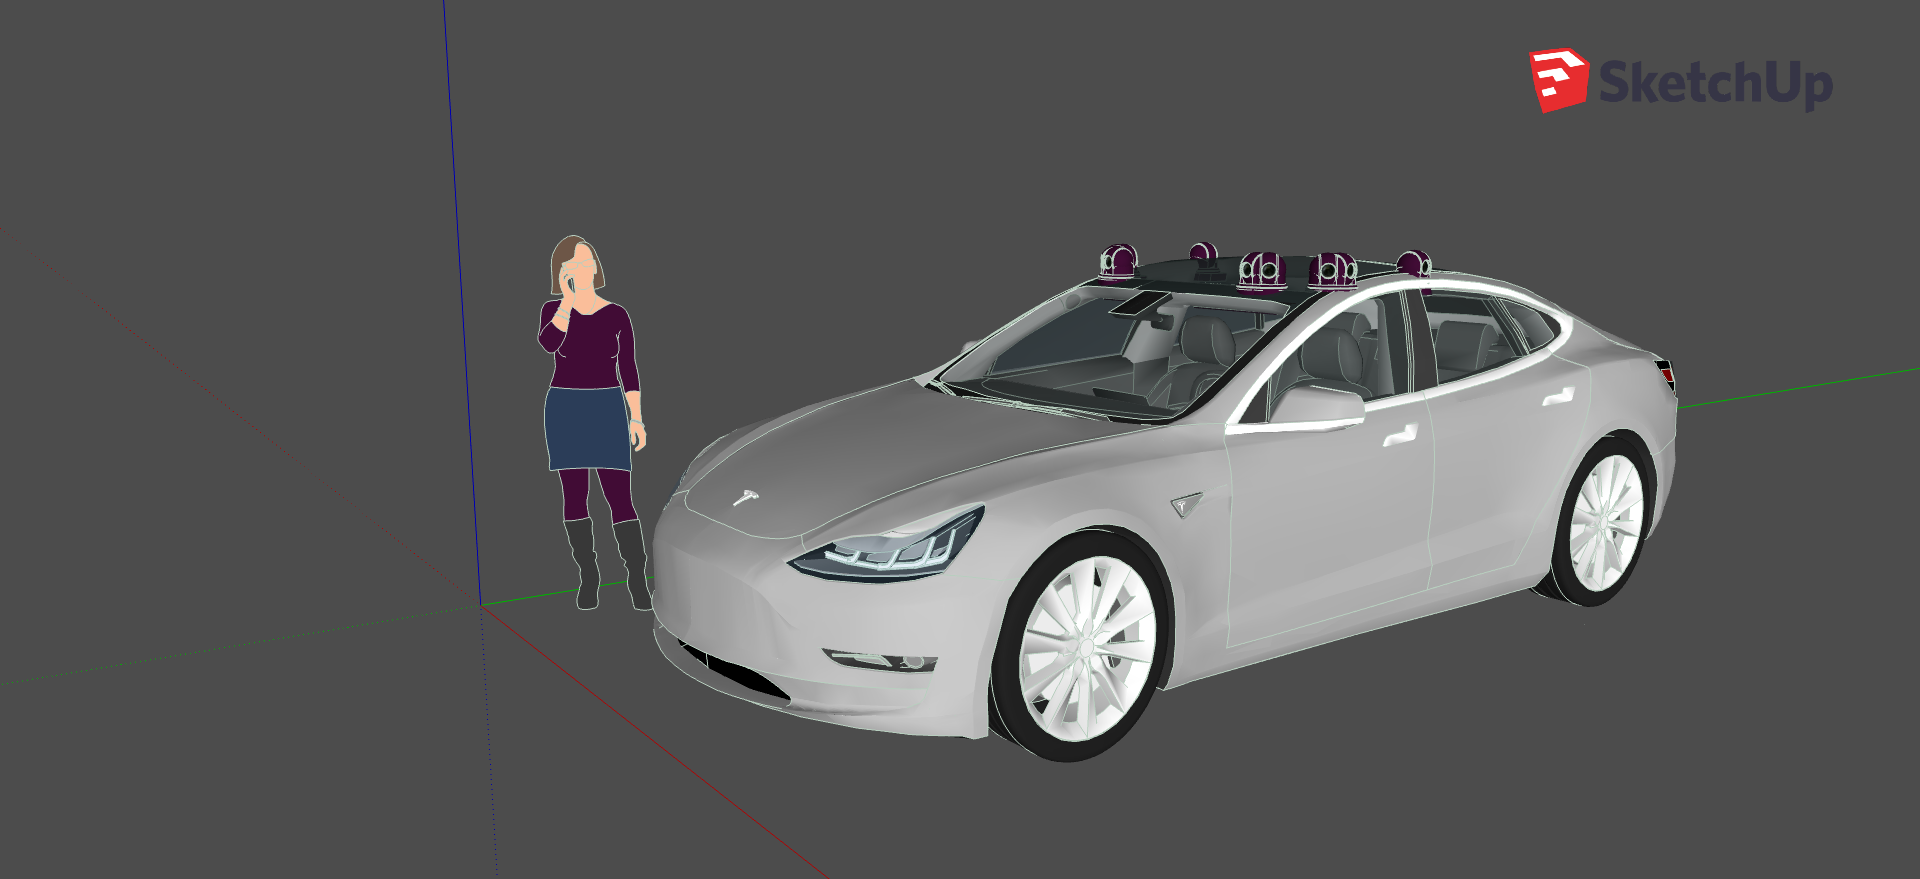
\includegraphics[width=67mm, keepaspectratio]{figures/3dmodel1.png}\hspace{1cm}
	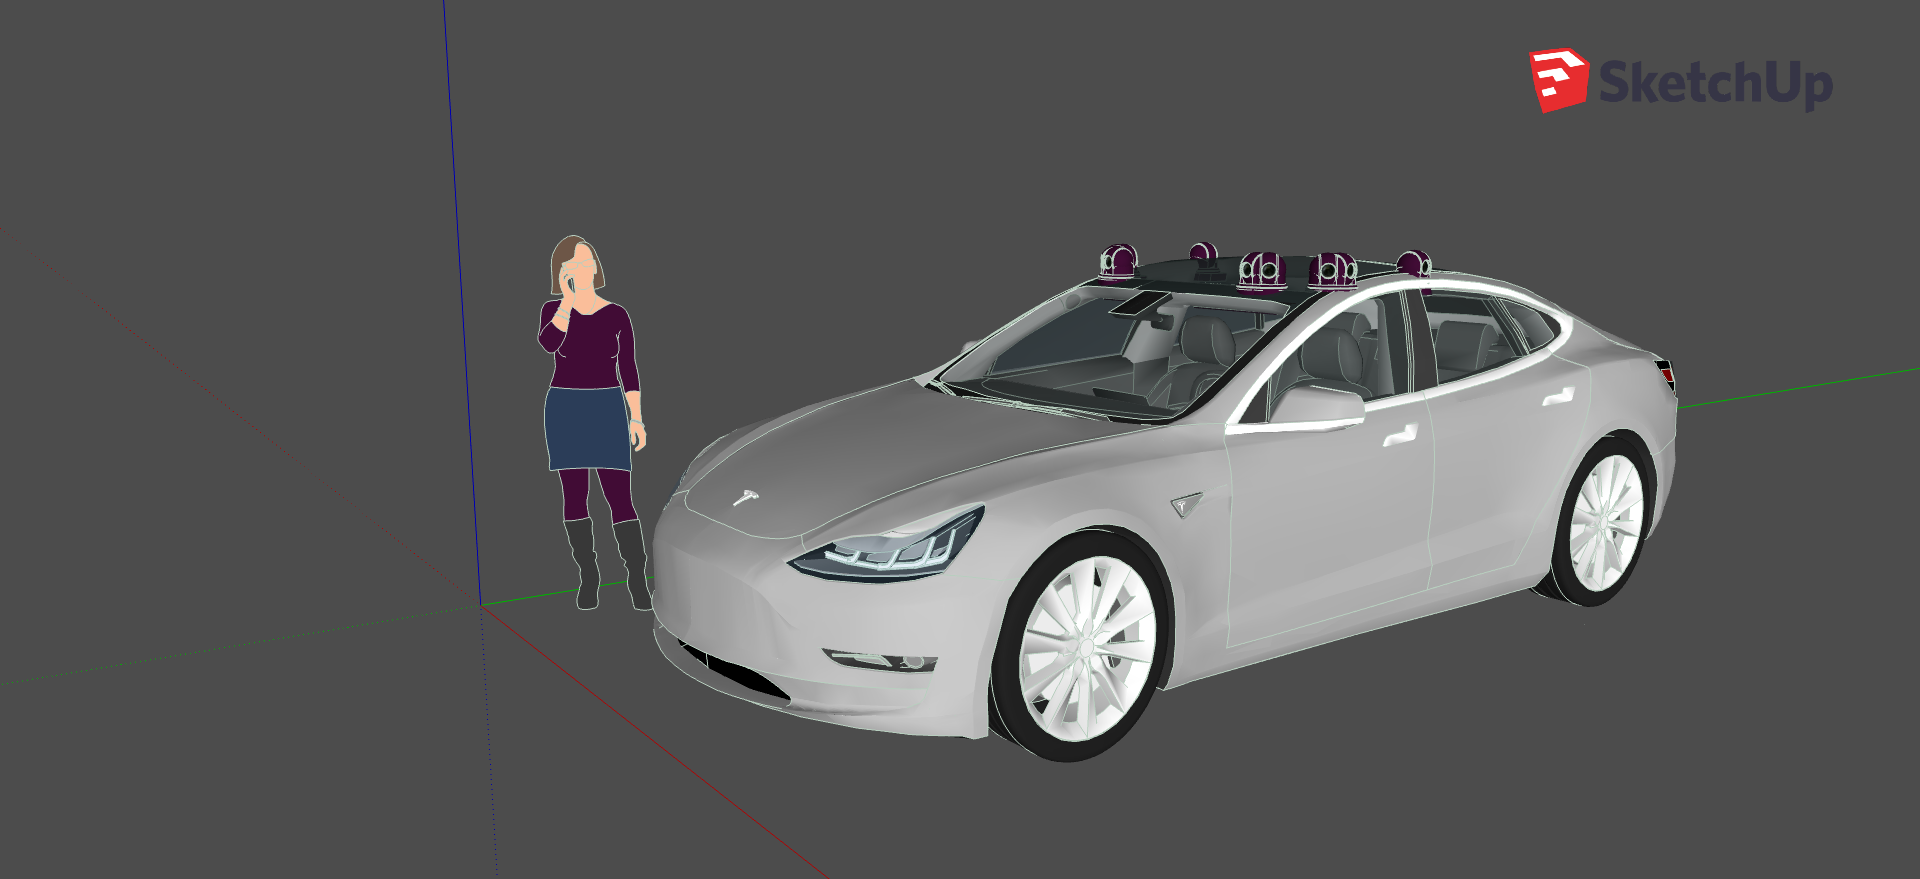
\includegraphics[width=67mm, keepaspectratio]{figures/3dmodel1.png}\\\vspace{5mm}
	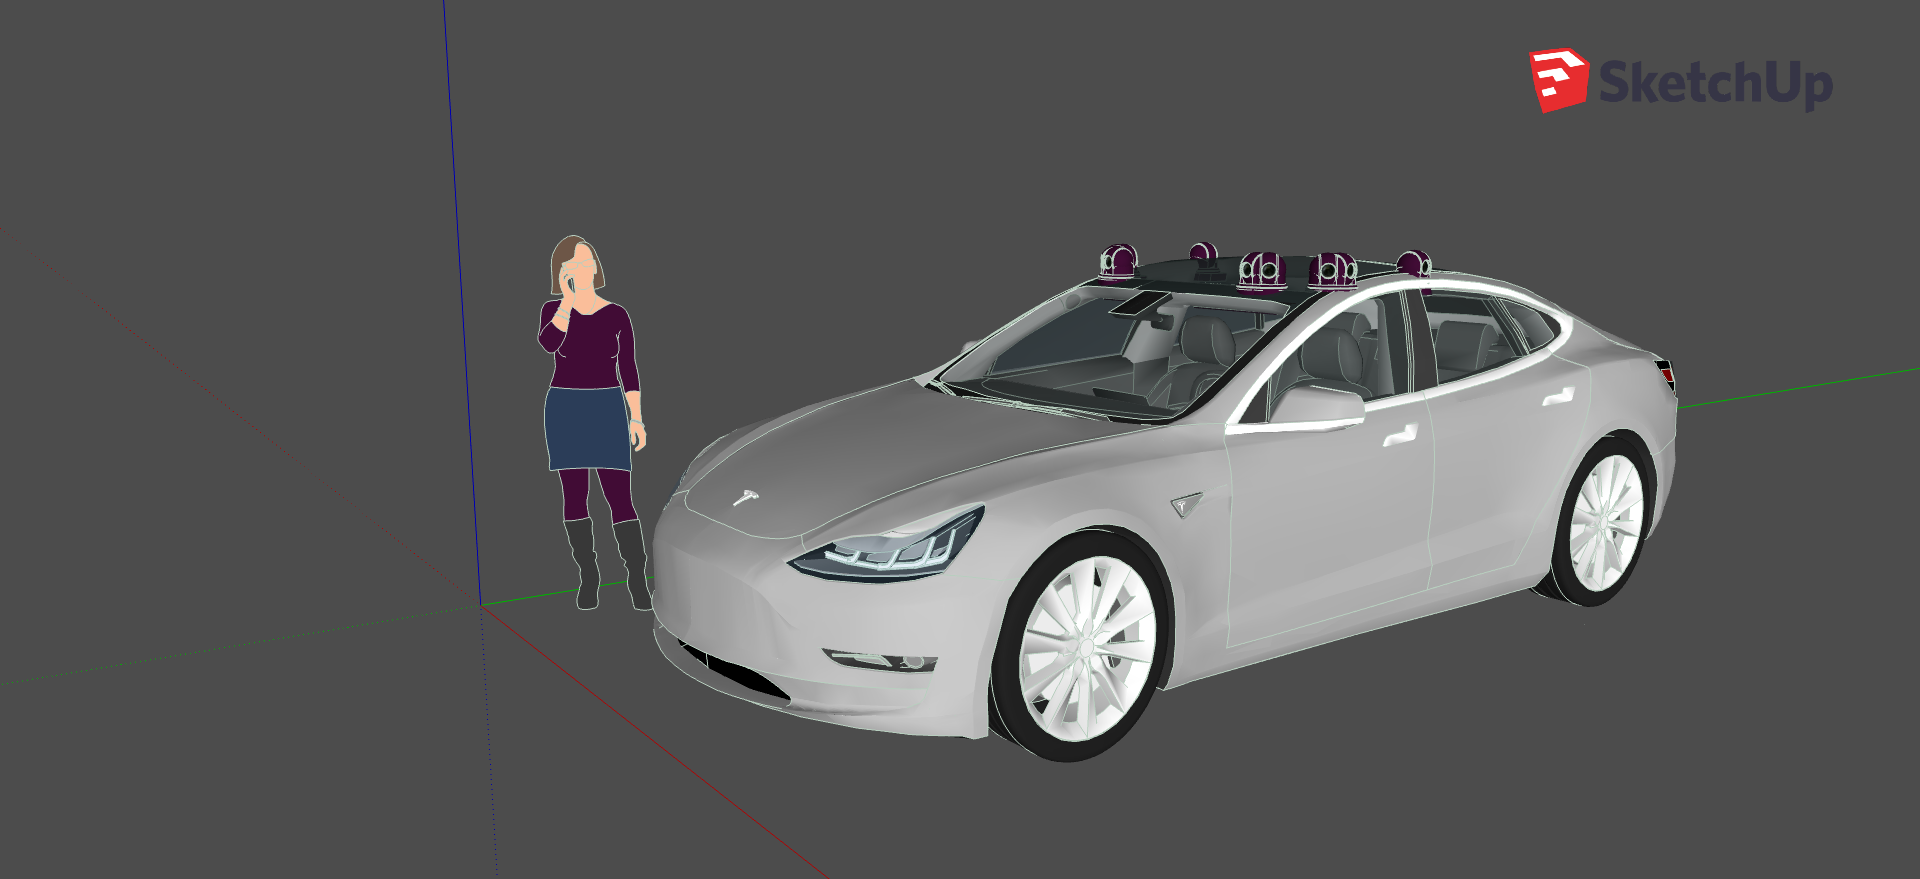
\includegraphics[width=67mm, keepaspectratio]{figures/3dmodel1.png}\hspace{1cm}
	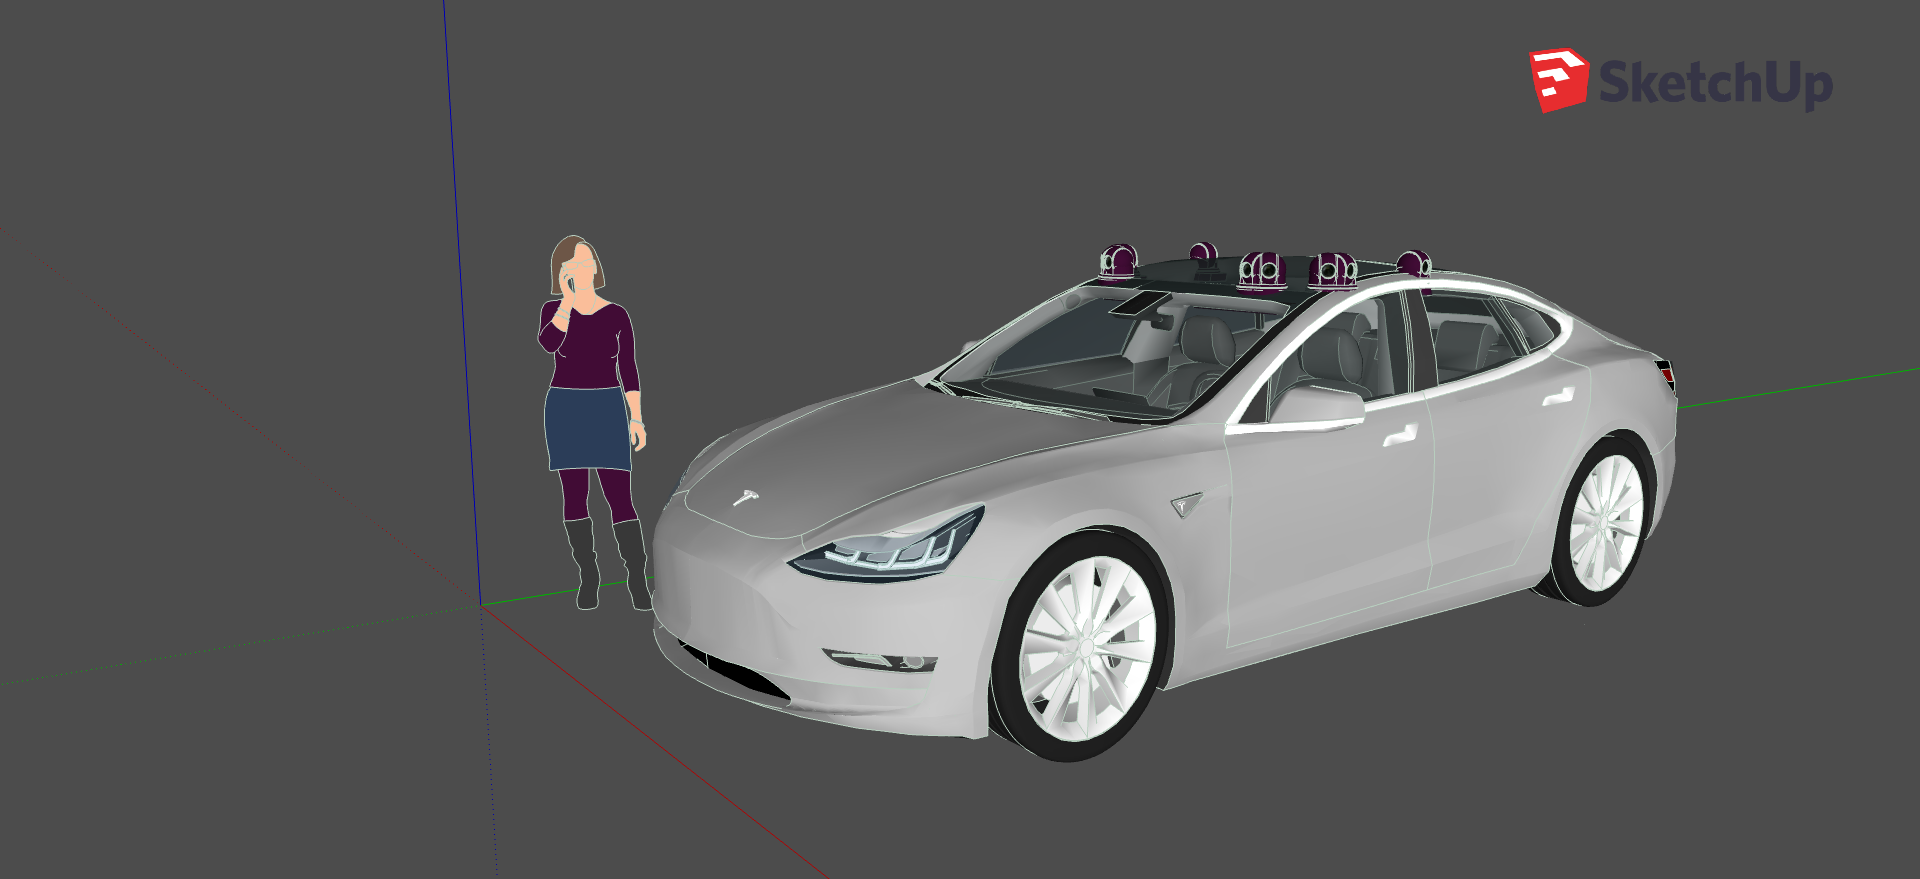
\includegraphics[width=67mm, keepaspectratio]{figures/3dmodel1.png}
	\caption{Több képfájl beillesztése esetén térközöket is érdemes használni.}
	\label{fig:HVSpaces}
\end{figure}

A táblázatok használatára \aref{tab:TabularExample}~táblázat mutat példát. A táblázatok formázásához hasznos tanácsokat találunk a \verb+booktabs+ csomag dokumentációjában.

\begin{table}[ht]
	\footnotesize
	\centering
	\begin{tabular}{ l c c }
		\toprule
		Órajel & Frekvencia & Cél pin \\
		\midrule
		CLKA & 100 MHz & FPGA CLK0\\
		CLKB & 48 MHz  & FPGA CLK1\\
		CLKC & 20 MHz  & Processzor\\
		CLKD & 25 MHz  & Ethernet chip \\
		CLKE & 72 MHz  & FPGA CLK2\\
		XBUF & 20 MHz  & FPGA CLK3\\
		\bottomrule
	\end{tabular}
	\caption{Az órajel-generátor chip órajel-kimenetei.}
	\label{tab:TabularExample}
\end{table}


%----------------------------------------------------------------------------
\section{Felsorolások és listák}
%----------------------------------------------------------------------------
Számozatlan felsorolásra mutat példát a jelenlegi bekezdés:
\begin{itemize}
	\item \emph{első bajusz:} ide lehetne írni az első elem kifejését,
	\item \emph{második bajusz:} ide lehetne írni a második elem kifejését,
	\item \emph{ez meg egy szakáll:} ide lehetne írni a harmadik elem kifejését.
\end{itemize}

Számozott felsorolást is készíthetünk az alábbi módon:
\begin{enumerate}
	\item \emph{első bajusz:} ide lehetne írni az első elem kifejését, és ez a kifejtés így néz ki, ha több sorosra sikeredik,
	\item \emph{második bajusz:} ide lehetne írni a második elem kifejését,
	\item \emph{ez meg egy szakáll:} ide lehetne írni a harmadik elem kifejését.
\end{enumerate}
A felsorolásokban sorok végén vessző, az utolsó sor végén pedig pont a szokásos írásjel. Ez alól kivételt képezhet, ha az egyes elemek több teljes mondatot tartalmaznak.

Listákban a dolgozat szövegétől elkülönítendő kódrészleteket, programsorokat, pszeudo-kódokat jeleníthetünk meg (\ref{lst:Example}.~kódrészlet).
\begin{lstlisting}[language=tex,caption=A fenti számozott felsorolás \LaTeX-forráskódja,label=lst:Example]
\begin{enumerate}
	\item \emph{els(*@ő@*) bajusz:} ide lehetne írni az els(*@ő@*) elem kifejését,
	és ez a kifejtés így néz ki, ha több sorosra sikeredik,
	\item \emph{második bajusz:} ide lehetne írni a második elem kifejését,
	\item \emph{ez meg egy szakáll:} ide lehetne írni a harmadik elem kifejését.
\end{enumerate}
\end{lstlisting}
A lista keretét, háttérszínét, egész stílusát megválaszthatjuk. Ráadásul különféle programnyelveket és a nyelveken belül kulcsszavakat is definiálhatunk, ha szükséges. Erről bővebbet a \verb+listings+ csomag hivatalos leírásában találhatunk.

%----------------------------------------------------------------------------
\section{Képletek}
%----------------------------------------------------------------------------
Ha egy formula nem túlságosan hosszú, és nem akarjuk hivatkozni a szövegből, mint például a $e^{i\pi}+1=0$ képlet, \emph{szövegközi képletként} szokás leírni. Csak, hogy másik példát is lássunk, az $U_i=-d\Phi/dt$ Faraday-törvény a $\rot E=-\frac{dB}{dt}$ differenciális alakban adott Maxwell-egyenlet felületre vett integráljából vezethető le. Látható, hogy a \LaTeX-fordító a sorközöket betartja, így a szöveg szedése esztétikus marad szövegközi képletek használata esetén is.

Képletek esetén az általános konvenció, hogy a kisbetűk skalárt, a kis félkövér betűk ($\mathbf{v}$) oszlopvektort -- és ennek megfelelően $\mathbf{v}^T$ sorvektort -- a kapitális félkövér betűk ($\mathbf{V}$) mátrixot jelölnek. Ha ettől el szeretnénk térni, akkor az alkalmazni kívánt jelölésmódot célszerű külön alfejezetben definiálni. Ennek megfelelően, amennyiben $\mathbf{y}$ jelöli a mérések vektorát, $\mathbf{\vartheta}$ a paraméterek vektorát és $\hat{\mathbf{y}}=\mathbf{X}\vartheta$ a paraméterekben lineáris modellt, akkor a \emph{Least-Squares} értelemben optimális paraméterbecslő $\hat{\mathbf{\vartheta}}_{LS}=(\mathbf{X}^T\mathbf{X})^{-1}\mathbf{X}^T\mathbf{y}$ lesz.

Emellett kiemelt, sorszámozott képleteket is megadhatunk, ennél az \verb+equation+ és a \verb+eqnarray+ környezetek helyett a korszerűbb \verb+align+ környezet alkalmazását javasoljuk (több okból, különféle problémák elkerülése végett, amelyekre most nem térünk ki). Tehát
\begin{align}
\dot{\mathbf{x}}&=\mathbf{A}\mathbf{x}+\mathbf{B}\mathbf{u},\\
\mathbf{y}&=\mathbf{C}\mathbf{x},
\end{align}
ahol $\mathbf{x}$ az állapotvektor, $\mathbf{y}$ a mérések vektora és $\mathbf{A}$, $\mathbf{B}$ és $\mathbf{C}$ a rendszert leíró paramétermátrixok. Figyeljük meg, hogy a két egyenletben az egyenlőségjelek egymáshoz igazítva jelennek meg, mivel a mindkettőt az \& karakter előzi meg a kódban. Lehetőség van számozatlan kiemelt képlet használatára is, például
\begin{align}
\dot{\mathbf{x}}&=\mathbf{A}\mathbf{x}+\mathbf{B}\mathbf{u},\nonumber\\
\mathbf{y}&=\mathbf{C}\mathbf{x}\nonumber.
\end{align}
Mátrixok felírására az $\mathbf{A}\mathbf{x}=\mathbf{b}$ inhomogén lineáris egyenlet részletes kifejtésével mutatunk példát:
\begin{align}
\begin{bmatrix}
a_{11} & a_{12} & \dots & a_{1n}\\
a_{21} & a_{22} & \dots & a_{2n}\\
\vdots & \vdots & \ddots & \vdots\\
a_{m1} & a_{m2} & \dots & a_{mn}
\end{bmatrix}
\begin{pmatrix}x_1\\x_2\\\vdots\\x_n\end{pmatrix}=
\begin{pmatrix}b_1\\b_2\\\vdots\\b_m\end{pmatrix}.
\end{align}
A \verb+\frac+ utasítás hatékonyságát egy általános másodfokú tag átviteli függvényén keresztül mutatjuk be, azaz
\begin{align}
W(s)=\frac{A}{1+2T\xi s+s^2T^2}.
\end{align}
A matematikai mód minden szimbólumának és képességének a bemutatására természetesen itt nincs lehetőség, de gyors referenciaként hatékonyan használhatók a következő linkek:\\
\indent\url{http://www.artofproblemsolving.com/LaTeX/AoPS_L_GuideSym.php},\\
\indent\url{http://www.ctan.org/tex-archive/info/symbols/comprehensive/symbols-a4.pdf},\\
\indent\url{ftp://ftp.ams.org/pub/tex/doc/amsmath/short-math-guide.pdf}.\\
Ez pedig itt egy magyarázat, hogy miért érdemes \verb+align+ környezetet használni:\\
\indent\url{http://texblog.net/latex-archive/maths/eqnarray-align-environment/}.

%----------------------------------------------------------------------------
\section{Irodalmi hivatkozások}
\label{sec:HowtoReference}
%----------------------------------------------------------------------------
Egy \LaTeX~dokumentumban az irodalmi hivatkozások definíciójának két módja van. Az egyik a \verb+\thebibliograhy+ környezet használata a dokumentum végén, az \verb+\end{document}+ lezárás előtt.
\begin{lstlisting}[language=tex]
\begin{thebibliography}{9}

\bibitem{Lamport94} Leslie Lamport, \emph{\LaTeX: A Document Preparation System}.
Addison Wesley, Massachusetts, 2nd Edition, 1994.

\end{thebibliography}
\end{lstlisting}

Ezek után a dokumentumban a \verb+\cite{Lamport94}+ utasítással hivatkozhatunk a forrásra. A fenti megadás viszonylag kötetlen, a szerző maga formázza az irodalomjegyzéket (ami gyakran inkonzisztens eredményhez vezet).

Egy sokkal professzionálisabb módszer a BiB\TeX{} használata, ezért ez a sablon is ezt támogatja. Ebben az esetben egy külön szöveges adatbázisban definiáljuk a forrásmunkákat, és egy külön stílusfájl határozza meg az irodalomjegyzék kinézetét. Ez, összhangban azzal, hogy külön formátumkonvenció határozza meg a folyóirat-, a könyv-, a konferenciacikk- stb. hivatkozások kinézetét az irodalomjegyzékben (a sablon használata esetén ezzel nem is kell foglalkoznia a hallgatónak, de az eredményt célszerű ellenőrizni). felhasznált hivatkozások adatbázisa egy \verb+.bib+ kiterjesztésű szöveges fájl, amelynek szerkezetét a \Aref{lst:Bibtex} kódrészlet demonstrálja. A forrásmunkák bevitelekor a sor végi vesszők külön figyelmet igényelnek, mert hiányuk a BiB\TeX-fordító hibaüzenetét eredményezi. A forrásmunkákat típus szerinti kulcsszó vezeti be (\verb+@book+ könyv, \verb+@inproceedings+ konferenciakiadványban megjelent cikk, \verb+@article+ folyóiratban megjelent cikk, \verb+@techreport+ valamelyik egyetem gondozásában megjelent műszaki tanulmány, \verb+@manual+ műszaki dokumentáció esetén stb.). Nemcsak a megjelenés stílusa, de a kötelezően megadandó mezők is típusról-típusra változnak. Egy jól használható referencia a \url{http://en.wikipedia.org/wiki/BibTeX} oldalon található.

\begin{lstlisting}[caption=Példa szöveges irodalomjegyzék-adatbázisra Bib\TeX{} használata esetén.,label=lst:Bibtex]
@book{Wettl04,
  author    = {Ferenc Wettl and Gyula Mayer and Péter Szabó},
  publisher = {Panem Könyvkiadó},
  title     = {\LaTeX~kézikönyv},
  year      = {2004},
}

@article{Candy86,
  author       = {James C. Candy},
  journaltitle = {{IEEE} Trans.\ on Communications},
  month        = {01},
  note         = {\doi{10.1109/TCOM.1986.1096432}},
  number       = {1},
  pages        = {72--76},
  title        = {Decimation for Sigma Delta Modulation},
  volume       = {34},
  year         = {1986},
}

@inproceedings{Lee87,
  author    = {Wai L. Lee and Charles G. Sodini},
  booktitle = {Proc.\ of the IEEE International Symposium on Circuits and Systems},
  location  = {Philadelphia, PA, USA},
  month     = {05~4--7},
  pages     = {459--462},
  title     = {A Topology for Higher Order Interpolative Coders},
  vol       = {2},
  year      = {1987},
}

@thesis{KissPhD,
  author      = {Peter Kiss},
  institution = {Technical University of Timi\c{s}oara, Romania},
  month       = {04},
  title       = {Adaptive Digital Compensation of Analog Circuit Imperfections for Cascaded Delta-Sigma Analog-to-Digital Converters},
  type        = {phdthesis},
  year        = {2000},
}

@manual{Schreier00,
  author       = {Richard Schreier},
  month        = {01},
  note         = {\url{http://www.mathworks.com/matlabcentral/fileexchange/}},
  organization = {Oregon State University},
  title        = {The Delta-Sigma Toolbox v5.2},
  year         = {2000},
}

@misc{DipPortal,
  author       = {{Budapesti Műszaki és Gazdaságtudományi Egyetem Villamosmérnöki és Informatikai Kar}},
  howpublished = {\url{http://diplomaterv.vik.bme.hu/}},
  title        = {Diplomaterv portál (2011. február 26.)},
}

@incollection{Mkrtychev:1997,
  author    = {Mkrtychev, Alexey},
  booktitle = {Logical Foundations of Computer Science},
  doi       = {10.1007/3-540-63045-7_27},
  editor    = {Adian, Sergei and Nerode, Anil},
  isbn      = {978-3-540-63045-6},
  pages     = {266-275},
  publisher = {Springer Berlin Heidelberg},
  series    = {Lecture Notes in Computer Science},
  title     = {Models for the logic of proofs},
  url       = {http://dx.doi.org/10.1007/3-540-63045-7_27},
  volume    = {1234},
  year      = {1997},
}
\end{lstlisting}

A stílusfájl egy \verb+.sty+ kiterjesztésű fájl, de ezzel lényegében nem kell foglalkozni, mert vannak beépített stílusok, amelyek jól használhatók. Ez a sablon a BiB\TeX-et használja, a hozzá tartozó adatbázisfájl a \verb+mybib.bib+ fájl. Megfigyelhető, hogy az irodalomjegyzéket a dokumentum végére (a \verb+\end{document}+ utasítás elé) beillesztett \verb+\bibliography{mybib}+ utasítással hozhatjuk létre, a stílusát pedig ugyanitt a  \verb+\bibliographystyle{plain}+ utasítással adhatjuk meg. Ebben az esetben a \verb+plain+ előre definiált stílust használjuk (a sablonban is ezt állítottuk be). A \verb+plain+ stíluson kívül természetesen számtalan más előre definiált stílus is létezik. Mivel a \verb+.bib+ adatbázisban ezeket megadtuk, a BiB\TeX-fordító is meg tudja különböztetni a szerzőt a címtől és a kiadótól, és ez alapján automatikusan generálódik az irodalomjegyzék a stílusfájl által meghatározott stílusban.

Az egyes forrásmunkákra a szövegből továbbra is a \verb+\cite+ paranccsal tudunk hivatkozni, így \aref{lst:Bibtex}.~kódrészlet esetén a hivatkozások rendre \verb+\cite{Wettl04}+, \verb+\cite{Candy86}+, \verb+\cite{Lee87}+, \verb+\cite{KissPhD}+, \verb+\cite{Schreirer00}+,
\verb+\cite{Mkrtychev:1997}+ és \verb+\cite{DipPortal}+. Az egyes forrásmunkák sorszáma az irodalomjegyzék bővítésekor változhat. Amennyiben az aktuális számhoz illeszkedő névelőt szeretnénk használni, használjuk az \verb+\acite{}+ parancsot.

Az irodalomjegyzékben alapértelmezésben csak azok a forrásmunkák jelennek meg, amelyekre található hivatkozás a szövegben, és ez így alapvetően helyes is, hiszen olyan forrásmunkákat nem illik az irodalomjegyzékbe írni, amelyekre nincs hivatkozás.

Mivel a fordítási folyamat során több lépésben oldódnak fel a szimbólumok, ezért gyakran többször is le kell fordítani a dokumentumot. Ilyenkor ez első 1-2 fordítás esetleg szimbólum-feloldásra vonatkozó figyelmeztető üzenettel zárul. Ha hibaüzenettel zárul bármelyik fordítás, akkor nincs értelme megismételni, hanem a hibát kell megkeresni. A \verb+.bib+ fájl megváltoztatáskor sokszor nincs hatása a változtatásnak azonnal, mivel nem mindig fut újra a BibTeX fordító. Ezért célszerű a változtatás után azt manuálisan is lefuttatni (TeXstudio esetén \verb+Tools/Bibliography+).

Hogy a szövegbe ágyazott hivatkozások kinézetét demonstráljuk, itt most sorban meghivatkozzuk a \cite{Wettl04}, \cite{Candy86}, \cite{Lee87}, \cite{KissPhD}, \cite{Schreier00} és \acite{Mkrtychev:1997}\footnote{Informatikai témában gyakran hivatkozunk cikkeket a Springer LNCS valamely kötetéből, ez a hivatkozás erre mutat egy helyes példát.} forrásmunkát, valamint \acite{DipPortal} weboldalt.

Megjegyzendő, hogy az ékezetes magyar betűket is tartalmazó \verb+.bib+ fájl az \verb+inputenc+ csomaggal betöltött \verb+latin2+ betűkészlet miatt fordítható. Ugyanez a \verb+.bib+ fájl hibaüzenettel fordul egy olyan dokumentumban, ami nem tartalmazza a \verb+\usepackage[latin2]{inputenc}+ sort. Speciális igény esetén az irodalmi adatbázis általánosabb érvényűvé tehető, ha az ékezetes betűket speciális latex karakterekkel helyettesítjük a \verb+.bib+ fájlban, pl. á helyett \verb+\'{a}+-t vagy ő helyett \verb+\H{o}+-t írunk.

Irodalomhivatkozásokat célszerű először olyan szolgáltatásokban keresni, ahol jó minőségű bejegyzések találhatók (pl. ACM Digital Library,\footnote{\url{https://dl.acm.org/}} DBLP,\footnote{\url{http://dblp.uni-trier.de/}} IEEE Xplore,\footnote{\url{http://ieeexplore.ieee.org/}} SpringerLink\footnote{\url{https://link.springer.com/}}) és csak ezek után használni kevésbé válogatott forrásokat (pl. Google Scholar\footnote{\url{http://scholar.google.com/}}). A jó minőségű bejegyzéseket is érdemes megfelelően tisztítani.\footnote{\url{https://github.com/FTSRG/cheat-sheets/wiki/BibTeX-Fixing-entries-from-common-sources}} A sablon angol nyelvű változatában használt \texttt{plainnat} beállítás egyik sajátossága, hogy a cikkhez generált hivatkozás a cikk DOI-ját és URL-jét is tartalmazza, ami gyakran duplikátumhoz vezet -- érdemes tehát a DOI-kat tartalmazó URL mezőket törölni. 

%----------------------------------------------------------------------------
\section{A dolgozat szerkezete és a forrásfájlok}
%----------------------------------------------------------------------------
A diplomatervsablonban a TeX fájlok két alkönyvtárban helyezkednek el. Az \verb+include+ könyvtárban azok szerepelnek, amiket tipikusan nem kell szerkesztenünk, ezek a sablon részei (pl. címoldal). A \verb+content+ alkönyvtárban pedig a saját munkánkat helyezhetjük el. Itt érdemes az egyes fejezeteket külön \TeX{} állományokba rakni.

A diplomatervsablon (a kari irányelvek szerint) az alábbi fő fejezetekből áll:
\begin{enumerate}
	\item 1 oldalas \emph{tájékoztató} a szakdolgozat/diplomaterv szerkezetéről (\verb+include/guideline.tex+), ami a végső dolgozatból törlendő,
	\item \emph{feladatkiírás} (\verb+include/project.tex+), a dolgozat nyomtatott verzójában ennek a helyére kerül a tanszék által kiadott, a tanszékvezető által aláírt feladatkiírás, a dolgozat elektronikus verziójába pedig a feladatkiírás egyáltalán ne kerüljön bele, azt külön tölti fel a tanszék a diplomaterv-honlapra,
	\item \emph{címoldal} (\verb+include/titlepage.tex+),
	\item \emph{tartalomjegyzék} (\verb+thesis.tex+),
	\item a diplomatervező \emph{nyilatkozat}a az önálló munkáról (\verb+include/declaration.tex+),
	\item 1-2 oldalas tartalmi \emph{összefoglaló} magyarul és angolul, illetve elkészíthető még további nyelveken is (\verb+content/abstract.tex+),
	\item \emph{bevezetés}: a feladat értelmezése, a tervezés célja, a feladat indokoltsága, a diplomaterv felépítésének rövid összefoglalása (\verb+content/introduction.tex+),
	\item sorszámmal ellátott \emph{fejezetek}: a feladatkiírás pontosítása és részletes elemzése, előzmények (irodalomkutatás, hasonló alkotások), az ezekből levonható következtetések, a tervezés részletes leírása, a döntési lehetőségek értékelése és a választott megoldások indoklása, a megtervezett műszaki alkotás értékelése, kritikai elemzése, továbbfejlesztési lehetőségek,
	\item esetleges \emph{köszönetnyilvánítás}ok (\verb+content/acknowledgement.tex+),
	\item részletes és pontos \emph{irodalomjegyzék} (ez a sablon esetében automatikusan generálódik a \verb+thesis.tex+ fájlban elhelyezett \verb+\bibliography+ utasítás hatására, \az+\refstruc{sec:HowtoReference}ban leírtak szerint),
	\item \emph{függelékek} (\verb+content/appendices.tex+).
\end{enumerate}

A sablonban a fejezetek a \verb+thesis.tex+ fájlba vannak beillesztve \verb+\include+ utasítások segítségével. Lehetőség van arra, hogy csak az éppen szerkesztés alatt álló \verb+.tex+ fájlt fordítsuk le, ezzel lerövidítve a fordítási folyamatot. Ezt a lehetőséget az alábbi kódrészlet biztosítja a \verb+thesis.tex+ fájlban.
\begin{lstlisting}
\includeonly{
	guideline,%
	project,%
	titlepage,%
	declaration,%
	abstract,%
	introduction,%
	chapter1,%
	chapter2,%
	chapter3,%
	acknowledgement,%
	appendices,%
}
\end{lstlisting}

Ha az alábbi kódrészletben az egyes sorokat a \verb+%+ szimbólummal kikommentezzük, akkor a megfelelő \verb+.tex+ fájl nem fordul le. Az oldalszámok és a tartalomjegyék természetesen csak akkor billennek helyre, ha a teljes dokumentumot lefordítjuk.

%----------------------------------------------------------------------------
\newpage
\section{Alapadatok megadása}
%----------------------------------------------------------------------------
A diplomaterv alapadatait (cím, szerző, konzulens, konzulens titulusa) a \verb+thesis.tex+ fájlban lehet megadni.

%----------------------------------------------------------------------------
\section{Új fejezet írása}
%----------------------------------------------------------------------------
A főfejezetek külön \verb+content+ könyvtárban foglalnak helyet. A sablonhoz 3 fejezet készült. További főfejezeteket úgy hozhatunk létre, ha új \TeX~fájlt készítünk a fejezet számára, és a \verb+thesis.tex+ fájlban, a \verb+\include+ és \verb+\includeonly+ utasítások argumentumába felvesszük az új \verb+.tex+ fájl nevét.


%----------------------------------------------------------------------------
\section{Definíciók, tételek, példák}
%----------------------------------------------------------------------------

\begin{definition}[Fluxuskondenzátor térerőssége]
Lorem ipsum dolor sit amet, consectetur adipiscing elit, sed do eiusmod tempor incididunt ut labore et dolore magna aliqua. Ut enim ad minim veniam, quis nostrud exercitation ullamco laboris nisi ut aliquip ex ea commodo consequat.
\end{definition}

\begin{example}
Példa egy példára. Duis aute irure dolor in reprehenderit in voluptate velit esse cillum dolore eu fugiat nulla pariatur. Excepteur sint occaecat cupidatat non proident, sunt in culpa qui officia deserunt mollit anim id est laborum.
\end{example}

\begin{theorem}[Kovács tétele]
Duis aute irure dolor in reprehenderit in voluptate velit esse cillum dolore eu fugiat nulla pariatur. Excepteur sint occaecat cupidatat non proident, sunt in culpa qui officia deserunt mollit anim id est laborum.
\end{theorem}




% Bibliography
%~~~~~~~~~~~~~~~~~~~~~~~~~~~~~~~~~~~~~~~~~~~~~~~~~~~~~~~~~~~~~~~~~~~~~~~~~~~~~~~~~~~~~~
\addcontentsline{toc}{chapter}{\bibname}
\bibliography{bib/mybib}

% Appendix
%~~~~~~~~~~~~~~~~~~~~~~~~~~~~~~~~~~~~~~~~~~~~~~~~~~~~~~~~~~~~~~~~~~~~~~~~~~~~~~~~~~~~~~
% %----------------------------------------------------------------------------
\appendix
%----------------------------------------------------------------------------
\chapter*{\fuggelek}\addcontentsline{toc}{chapter}{\fuggelek}
\setcounter{chapter}{\appendixnumber}
%\setcounter{equation}{0} % a fofejezet-szamlalo az angol ABC 6. betuje (F) lesz
\numberwithin{equation}{section}
\numberwithin{figure}{section}
\numberwithin{lstlisting}{section}
%\numberwithin{tabular}{section}



\end{document}